%% LyX 2.4.3 created this file.  For more info, see https://www.lyx.org/.
%% Do not edit unless you really know what you are doing.
\documentclass[english,12pt]{article}
\usepackage[T1]{fontenc}
\usepackage[latin9]{inputenc}
\usepackage{babel}
\usepackage{verbatim}
\usepackage{mathrsfs}
\usepackage{mathtools}
\usepackage{amsmath}
\usepackage{amsthm}
\usepackage{amssymb}
\usepackage{stackrel}
\usepackage{graphicx}
\usepackage{geometry}
\geometry{verbose}
\usepackage{setspace}
\usepackage[authoryear]{natbib}
\PassOptionsToPackage{normalem}{ulem}
\usepackage{ulem}
\onehalfspacing
\usepackage[]
 {hyperref}

\makeatletter

%%%%%%%%%%%%%%%%%%%%%%%%%%%%%% LyX specific LaTeX commands.
\newcommand{\noun}[1]{\textsc{#1}}

%%%%%%%%%%%%%%%%%%%%%%%%%%%%%% Textclass specific LaTeX commands.
\theoremstyle{plain}
\newtheorem{prop}{\protect\propositionname}
\theoremstyle{plain}
\newtheorem{lem}{\protect\lemmaname}
\newcounter{atable}
\newcounter{afigure}
\newcounter{assumption}

%%%%%%%%%%%%%%%%%%%%%%%%%%%%%% User specified LaTeX commands.
\usepackage[T1]{fontenc}
\usepackage[latin9]{inputenc}
\usepackage{amsmath, amsthm, amssymb}
\usepackage{graphicx}
\usepackage{setspace}
\usepackage{natbib}
\PassOptionsToPackage{normalem}{ulem}
\usepackage{appendix}
\usepackage{ragged2e}
\usepackage{hyperref}
\usepackage[dvipsnames,svgnames,x11names,hyperref]{xcolor}
\hypersetup{colorlinks = true, urlcolor=MidnightBlue, citecolor=MidnightBlue}
\usepackage[noabbrev]{cleveref}
\usepackage{ulem}
\onehalfspacing
\makeatletter


%%%%%%%%%%%%%%%%%%%%%%%%%%%%%% User-specified LaTeX commands.
% Already loaded near the top; reloading with options causes a clash on modern TeX Live.
%\usepackage[english]{babel}
\usepackage{amsmath,amssymb,amsfonts}
\usepackage[scaled=1]{helvet}
\usepackage{mathpazo}
%\usepackage[margin=0.5in]{geometry}
\usepackage{ifthen}
\@ifpackageloaded{geometry}
  {\geometry{margin=1.1in}}
  {\usepackage[margin=1.1in]{geometry}}




\usepackage{array}
\usepackage{stmaryrd}
\usepackage[T1]{fontenc}
\usepackage{palatino}
\usepackage{mathtools}
\usepackage{multirow,booktabs}

\makeatother

\usepackage{authblk}
\usepackage[scr=boondox,cal=cm]{mathalpha}

\author{%
\makebox[\linewidth][c]{%
  \begin{minipage}{0.3\linewidth}\centering
    Siying Ding \\ \vspace{-0.5em}
    {\small \textit{UIBE}}
  \end{minipage}
  \hspace{1em}
  \begin{minipage}{0.35\linewidth}\centering
    Ahmad Lashkaripour \\ \vspace{-0.5em}
    {\small \textit{Indiana University, CESifo, CEPR}}
  \end{minipage}
  \hspace{1em}
  \begin{minipage}{0.35\linewidth}\centering
    Volodymyr Lugovskyy \\ \vspace{-0.5em}
    {\small \textit{Indiana University}}
  \end{minipage}
}%
}

\date{}
%\date{First version: August 2021 \\ This version: July 2022}
%\date{August 2023 \\ \textcolor{blue}{[Preliminary and Incomplete: Please do not circulate.]}}

\usepackage{tikz}
\usetikzlibrary{patterns}
\usepackage{subcaption}
\usepackage{pgfplots}
\pgfplotsset{compat=1.18}
\usepackage{colortbl}


\usepackage{tabularx} 
\usepackage{siunitx} 
\usepackage{adjustbox}

\makeatother

\providecommand{\lemmaname}{Lemma}
\providecommand{\propositionname}{Proposition}

\begin{document}
\title{Markups as Shadow Tariffs: \\ How Market Power Skews Trade Reciprocity}
\maketitle
\begin{abstract}
We show that in open economies, firm markups function as shadow tariffs:
they generate domestic deadweight losses but also shift surplus internationally
through excess profits earned abroad. These international profit-shifting
effects represent a pure distributive externality, benefiting countries
that capture a larger share of global excess profits. We derive a
new formula for the welfare loss from market power under these distributive
externalities and compile global data on firm markups and multinational
ownership to measure the tariff-equivalent of observed markups. Our
findings reveal that high-income countries capture a disproportionate
share of global excess profits. Consequently, the welfare losses from
market power for these countries are mitigated, and in some cases
reversed, through net profit inflows from abroad. We estimate that
these profit-shifting externalities are equivalent to a 17.6 percent
shadow tariff imposed by high-income countries---challenging the
view that advanced countries have made outsized concessions under
existing trade agreements.
\end{abstract}

\section{Introduction}

Growing trade integration and market power are two defining features
of today's global economy. Taken together, they raise a basic question:
are the welfare losses from market power localized, or do they spill
over internationally through increased trade integration? Current
research provides no clear answer. The literature has largely focused
on how trade integration curbs market power through pro-competitive
pressures. Far less attention has been paid to spillover effects:
whether the burden of market power has shifted internationally through
trade relations. If such spillovers exist, they amount to an international
externality, the kind that cannot be addressed by domestic policy
alone.

This paper explores this often overlooked aspect of global market
power. Our central thesis is that firm markups generate significant
international spillover effects, making them functionally equivalent
to import tariffs. Like tariffs, markups introduce a domestic deadweight
loss. But they also create distributive beggar-thy-neighbor effects:
monopolistic markups shift surplus from foreign consumers to domestic
firms through excess profits earned abroad. We show that, under fairly
general conditions, there exists a shadow tariff schedule that replicates
the aggregate welfare effects of markups. 

Our analysis begins with a theoretical welfare decomposition that
separates the aggregate loss from market power into two parts: $(i)$
the conventional deadweight loss from markup dispersion, and $(ii)$
a distributive profit-shifting externality. The latter mirrors classic
terms of trade effects: it benefits countries that capture a larger
share of global excess profits at the expense of others. 

We measure these distributive profit-shifting effects empirically
and test our equivalence result using newly compiled data on firm
markups and multinational ownership across countries. Our analysis
reveals that high-income economies collect a disproportionate share
of global excess profits. As a result, the welfare losses from market
power in these countries are partly, or in some cases entirely, counterbalanced
by incoming profits earned abroad. The Netherlands offers a particularly
bold example: although markups introduce the usual distortion to domestic
prices in this country, the inflow of foreign-raised excess profits
more than compensates for the loss in consumer surplus, yielding a
net aggregate welfare gain.

On average, we estimate that profit-shifting effects have attenuated
the aggregate welfare loss from market power in high-income countries
by roughly 15\%, precisely because these economies are net recipients
of global profit inflows. By contrast, lower-income countries that
experience net profit outflows face magnified welfare losses---approximately
44\% higher than they would in the absence of profit-shifting. These
equilibrium profit-shifting effects represent a \emph{shadow tariff}
of about 17.6 percent imposed by high-income nations on their trading
partners. In practice, such shadow tariffs erode, or even neutralize,
the non-reciprocal concessions that developed countries extend under
the WTO framework, challenging a growing line of criticism regarding
asymmetries in the global trading system.

Section \ref{sec: Baseline Model} presents our baseline semi-parametric
model of the global economy, which borrows elements from \citet{arkolakis2019elusive}
and \citet{errico2022quality}. Our baseline model features many countries
and industries. Firms apply variable and heterogeneous markups and
select into international markets \`a la \citet{melitz2008market}.
We also formalize and quantify extensions with firm entry dissipating
quasi-rents, multi-national ownership, and global input-output linkages.

Section \ref{sec: Cost of Markups} presents our sufficient statistics
formulas for the aggregate loss from market power under trade relations.
We show that the loss can be decomposed into $\left(i\right)$ an
entropy-based measure of markup dispersion, $(ii)$ changes to the
gains from trade due to markup-distorted relative factor prices, and
$(iii)$ zero-sum international profit-shifting effects. 

International profit-shifting effects are a pure distributive externality.
Our formula equates them to the ratio of the average expenditure-side
markup to the average output-side markup. This ratio diverges from
one due to a locational decoupling between where markups burden consumer
surplus and where the excess profits are remitted to households. As
a result of this decoupling, countries that collect a disproportionate
share of global excess profits experience a reduced loss due to net
profit inflows from abroad, while other countries endure a disproportionately
higher welfare loss due to net profit outflows.

Section \ref{sec: Implications-for-Policy} presents our duality result:
if countries are sufficiently open to trade, firm-level markups function
as shadow tariffs. The markups shift the terms of trade in favor of
countries that collect a greater share of global excess profits. We
establish this result in three steps. First, we show that a country
can unilaterally raise its welfare through a uniform markup on exports.
Second, we demonstrate that a centralized uniform markup on exports
is equivalent to an import tariff, echoing the Lerner symmetry. Third,
we show that the centralized markup or tariff yields higher welfare
gains than decentralized markups. Taking these results together, we
invoke the Intermediate Value Theorem to show that if trade levels
are sufficiently high, there exists a uniform tariff that replicates
the aggregate welfare effects of decentralized markups.

We calibrate our model using data described in Section \ref{sec: Quantitative }.
First, we construct novel data on multinational profit flows using
financial statements of multinational enterprises from the \noun{Orbis}
database. Second, we estimate global firm markups using two conventional
approaches: the cost-based method and the demand-based approach. For
the cost-based estimates, we use a global sample of publicly traded
firms from \noun{Worldscope}. Because performing structural demand
estimation at scale is challenging, we employ the computationally
efficient linear approximation of \citet{salanie2019fast}, and leverage
high-frequency transaction-level trade data to guide identification
despite limited information on product characteristics. We supplement
these firm-level data with international statistics on aggregate output,
expenditure, and sectoral input-output shares from the OECD Inter-Country
Input-Output (ICIO) tables. Combining these sources, we estimate (1)
markup dispersion, (2) expenditure-weighted average markup, (3) output-weighted
average markup, and (4) profit ownership shares across 64 major countries
plus an aggregate of the rest of the world over the period 2005--2015.

Using data on global markups and profit flows, we measure the aggregate
welfare loss from market power across many countries. We find that
these losses have modestly increased over time in most countries,
with markups reducing real consumption globally by more than 7\% in
2015. However, the losses are markedly larger among low-income countries.
In fact, some high-income countries, such as the Netherlands, even
benefit on net from market power because of sizable profit inflows
from abroad.

The North--South divide in welfare losses from market power is largely
driven by profit-shifting externalities. Net excess profit flows from
low-income to high-income countries have increased the burden of market
power for low-income economies by 44\%, while reducing the burden
for high-income countries by 15\%. This pattern is robust to alternative
assumptions about how markups are estimated, multinational ownership
structures, global input-output linkages, and fixed-cost payments.
These asymmetries reflect the fact that low-income countries tend
to specialize in less sophisticated, low-markup industries.

We estimate that international profit-shifting externalities are akin
to a 17.6\% shadow tariff imposed by high-income countries on their
trading partners. This finding sheds fresh light on the current state
of concessions within global trade agreements, challenging the growing
narrative that high-income countries, such as the United States, have
made disproportionately greater concessions under the status quo (\citealp{chow2018united}).
On a superficial level, high-income countries may appear to be making
additional concessions and offering preferential treatment to their
low-income counterparts under the WTO's Generalized System of Preferences
(GSP). But in reality, profit-shifting externalities more than counteract
the GSP concessions. After factoring in the implicit tariff due to
profit-shifting externalities, high-income countries are effectively
applying a 14\% \emph{excess} tariff on low-income partners. 

Our theoretical framework relates to a vibrant literature examining
the aggregate welfare loss from market power, and distortions more
broadly. A key insight from the early generation of studies, including
\citet{lerner1934concept} and \citet{harberger1954monopoly}, is
that aggregate welfare losses in closed economies are linked to markup
dispersion. Later work, such as \citet{hsieh2009misallocation}, \citet{baqaee2020productivity},
and \citet*{edmond2018costly} provide parametric formulas for these
aggregate welfare losses in closed-economy settings. There are limited
counterparts for these formulas in open-economy contexts. Several
studies including \citet{atkin2021role}, \citet{baqaee2024networks}
provide general frameworks for ex-ante growth accounting in distorted
open economies.\footnote{As in \citet*{arkolakis2019elusive}, pro-competitive effects are
essentially absent in our framework because the direct pro-competitive
effects on firm markups are exactly offset by firm-selection effects.
However, there is literature examining pro-competitive effects in
alternative settings, including \citet{melitz2008market}, \citet*{holmes2014allocative},
\citet{de2015understanding}, \citet*{edmond2015competition}, \citet{feenstra2017globalization}. } Relatedly, \citet*{bai2024misallocation} note that trade integration
can exacerbate misallocation in distorted economies, potentially worsening
aggregate welfare.\footnote{The idea that trade can exacerbate domestic misallocation has also
been explored by \citet{epifani2011trade}; \citet*{bai2019misallocation},
\citet{Manova2013}, \citet{farrokhi2024trade}, and \citet{dix2021trade}
in various contexts.} We contribute to this literature by proving a \emph{trade-adjusted}
formula for the aggregate welfare loss from markup distortions, emphasizing
the zero-sum profit-shifting effects, and establishing conditional
equivalence between firm markups and tariffs.

Our equivalence result is related to an old literature that converts
micro-level tariff wedges into one macro-level tariff index (\citet{anderson1996new,anderson2005measuring,anderson2003mercantilist,looi2009estimating,irwin2010trade,soderbery2021trade}).
Our approach is similar in that we convert micro-level wedges into
a representative tariff index. However, we differ from these papers
in important ways: we establish equivalence between decentralized
firm-level markups and a centralized tariff index. This equivalence
has implications for reciprocity and bilateral tariff concessions,
contributing to recent quantitative assessments of reciprocity as
in \citet*{bown2023reciprocity} and \citet{anderson2025tari}.

The profit-shifting externalities emphasized in this paper are related
but different from those in the strategic trade policy literature
(e.g., \citet{brander1985export,ossa2012profits,bagwell2012profit,lashkaripour2021cost,mrazova2024trade}).
In these frameworks profit-shifting is not an equilibrium externality,
but is strategically generated by government policies. More specifically,
government may use trade policy measures to promote high-profit activities
and strategically shift excess profits to their country. Our contribution
to this literature is to highlight the reverse aspect: We demonstrate
that decentralized pricing decisions by firms generate large distributive
externalities, yielding terms-of-trade benefits that, for some countries,
outweigh the domestic efficiency losses from markup pricing. As a
result, governments may purposefully avoid regulating firms to preserve
these implicit terms of trade benefits. \setlength{\abovedisplayskip}{10pt plus 1pt minus 1pt}
\setlength{\belowdisplayskip}{10pt plus 1pt minus 1pt}

\section{\label{sec: Basic-Calculus}Simple Illustration of Profit-Shifting
Externalities}

Before presenting our general model, we showcase the profit-shifting
mechanism using a simple model. There are two countries: North ($N$)
and South ($S$); and two traded sectors: a differentiated sector
and a homogeneous sector. The latter is indexed $0$ and is perfectly
competitive. The homogeneous good is traded and produced one-to-one
with labor in both countries. We assign the homogeneous good as the
numeraire ($p_{i,0}=p_{0}=1$) and assume that the homogeneous sector
is sufficiently large to have active production in both countries,
equalizing prices internationally. 

The utility function across industries is quasi-linear: $U_{i}=q_{i,0}+\frac{\alpha}{\beta}Q_{i}-\frac{1}{2\beta}Q_{i}^{2}$,
where $Q_{i}$ is a composite aggregator over differentiated firm
varieties and $q_{i,0}$ is the quantity of the homogeneous good.
Utility maximization implies a linear demand for the composite differentiated
good in each country:
\[
Q_{i}=\alpha-\beta P_{i}
\]
where $P_{i}$ is the price index of the composite differentiated
good in country $i$.\medskip{}

\noindent\emph{Production and markups in the differentiated sector}.$\quad$A
fixed measure $M_{i}\equiv\mid\Omega_{i}\mid$ of firms indexed by
$\omega\in\Omega_{i}$ supply the differentiated good in each country.
The firms are symmetric and monopolistically competitive. Each operates
with a common unit labor cost, $c$. The demand for firm varieties
of the differentiated good is CES. In particular, the consumption
aggregator is $Q_{i}=(\int_{\Omega_{i}}q_{\omega}^{\frac{\sigma-1}{\sigma}}d\omega)^{\frac{\sigma}{\sigma-1}}$,
yielding a constant elasticity demand for firm varieties: $q_{\omega}=p_{\omega}^{-\sigma}\times P_{i}^{\sigma}Q_{i}$.
The monopolistically competitive firms charge a constant markup $\mu=\frac{\sigma}{\sigma-1}$
over marginal cost $c$, implying a common firm-level price, $p_{\omega}=\mu\times c$.
The unit price for the composite differentiated good is thus:
\[
P_{i}=\mu\times c\times M_{i}^{\frac{1}{1-\sigma}}
\]
For simplicity, we assume henceforth that $M_{i}=1$, so that the
price of the composite differentiated good is equalized to $P\equiv\mu\times c$
in both countries. \medskip{}

\noindent\emph{Aggregate welfare loss from markups}.$\quad$ We now
characterize the aggregate welfare loss from markups, starting from
the closed economy case. As shown in the top panel of Figure \ref{fig: Textbook},
the aggregate welfare loss from markups for each country $i=N,S$
is the reduction in consumer surplus $\Delta CS_{i}$ minus the profit
rebates, $\frac{\mu-1}{\mu}PQ_{i}$. Namely,
\[
\mathscr{D}_{i}^{\left(closed\right)}=\,\Delta CS_{i}\,-\,\frac{\mu-1}{\mu}PQ_{i},
\]
Figure \ref{fig: Textbook} is a textbook digram: it states that the
losses coincides with the Harberger triangle. The intuition is that
excess profits in each country are ultimately rebated to consumers
as supplementary lump-sum transfers. Thus, the loss in consumer surplus
due to markups is partially offset by these rebates, leaving a residual
deadweight loss equal to the triangle.
\begin{figure}[!tbh]
\caption{\label{fig: Textbook}The welfare loss from market power: closed vs
open economies}
\vspace{-2.5pt}

\begin{centering}
\centering
\textbf{\large Closed Economy Case} \\
\begin{subfigure}{0.4\textwidth} 
\centering 
\begin{tikzpicture}[scale=0.575, every node/.style={font=\footnotesize}] 
\draw[->] (0,0) -- (11,0) node[right] {$Q$}; 
\draw[->] (0,0) -- (0,6) node[above] {$P$};
\draw (0,5) -- (10,0);         
\draw[dashed] (3.5,3.25) -- (3.5,0) node[below] {$Q_S$};       
 \draw[dashed] (8,1) -- (8,0) node[below] {$Q_{S}^{*}$};                
 \draw (0,1) -- (8,1);       
 \draw (0,3.25) -- (3.5,3.25);                  % Color the rectangle         
\fill[blue!50!teal, fill opacity=0.3] (0,1) rectangle (3.5,3.25);                  % Color the triangle         
\fill[orange!50!yellow, fill opacity=0.3] (3.5,1) -- (3.5,3.25) -- (8,1) -- cycle;                  % Color the trapezoid        
\fill[pattern=dots, fill opacity=0.3] (0,1) -- (0,3.25) -- (3.5,3.25) -- (8,1) -- cycle;                
 \node at (4.9,1.75) {$\mathscr{D}_{S}^{\left(closed\right)}$};        
\node at (1.5,2.75) {profits};        
\node at (1.75,1.75) {$S \rightarrow S$};        
\node[left] at (0,3.25) {$\mu \times c$};      
 \node[left] at (0,1) {$c$};  
\end{tikzpicture}    
\caption*{\large Country S} 
\end{subfigure} 
\hfill 
\begin{subfigure}{0.4\textwidth}    
\centering    
\begin{tikzpicture}[scale=0.575, every node/.style={font=\footnotesize}]         
\draw[->] (0,0) -- (11,0) node[right] {$Q$};   
\draw[->] (0,0) -- (0,6) node[above] {$P$};         
\draw (0,5) -- (10,0);        
\draw[dashed] (3.5,3.25) -- (3.5,0) node[below] {$Q_{N}$};       
 \draw[dashed] (8,1) -- (8,0) node[below] {$Q_{N}^{*}$};                 
\draw (0,1) -- (8,1);        
\draw (0,3.25) -- (3.5,3.25);                  % Color the rectangle        
\fill[red!50!orange, fill opacity=0.3] (0,1) rectangle (3.5,3.25);                  % Color the triangle         
\fill[orange!50!yellow, fill opacity=0.3] (3.5,1) -- (3.5,3.25) -- (8,1) -- cycle;                  % Color the trapezoid        
\fill[pattern=dots, fill opacity=0.3] (0,1) -- (0,3.25) -- (3.5,3.25) -- (8,1) -- cycle;                
 \node at (4.9,1.75) {$\mathscr{D}_{N}^{\left(closed\right)}$};         
\node at (1.5,2.75) {profits};        
\node at (1.75,1.75) {$N \rightarrow N$};       
 \node[left] at (0,3.25) {$\mu \times c$};        
\node[left] at (0,1) {$c$}; 

% Legend               
\node[anchor=north west, font=\small] at (3,6) {             
\begin{tabular}{c@{\hspace{0.2em}}l}                 
\tikz\draw[fill=white, pattern=dots] (0,0) rectangle (0.85,0.3); & $\Delta Consumer \ Surplus$            
\end{tabular}        
}; 

\end{tikzpicture}     
\caption*{\large Country N} 
\end{subfigure}
\par\end{centering}
\begin{centering}
\centering
\textbf{\large Open Economy Case} \\
\begin{subfigure}{0.4\textwidth} 
\centering 
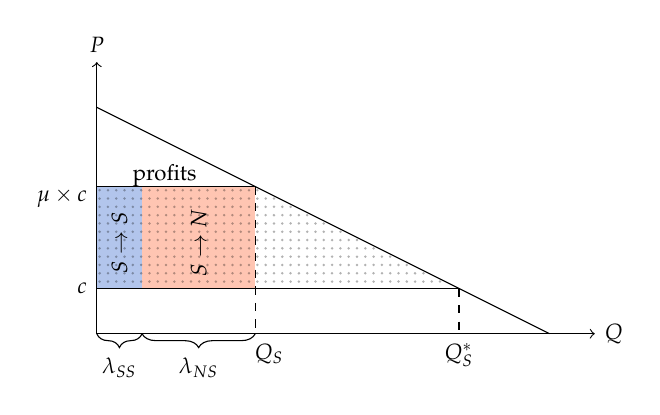
\begin{tikzpicture}[scale=0.575, every node/.style={font=\footnotesize}] 
\draw[->] (0,0) -- (11,0) node[right] {$Q$}; 
\draw[->] (0,0) -- (0,6) node[above] {$P$}; 
\draw (0,5) -- (10,0); 
\draw[dashed] (3.5,3.25) -- (3.5,0) node[below] {$\ \ \ \ \ Q_{S}$};       
 \draw[dashed] (8,1) -- (8,0) node[below] {$Q_{S}^{*}$};  
\draw (0,1) -- (8,1); 
\draw (0,3.25) -- (3.5,3.25); % Color the rectangle 
\fill[blue!50!teal, fill opacity=0.3] (0,1) rectangle (1,3.25); % Color the triangle 
\fill[red!50!orange, fill opacity=0.3] (1,1) rectangle (3.5,3.25); % Color the triangle 
%\fill[blue!30, fill opacity=0.3] (4,1) -- (3.5,3.25) -- (8,1) -- cycle; % Color the trapezoid 
\fill[pattern=dots, fill opacity=0.3] (0,1) -- (0,3.25) -- (3.5,3.25) -- (8,1) -- cycle; 
\node at (5.25,1.75) {};
\node at (1.5,3.5) {profits};
\node[rotate=90] at (0.5, 2) {$S \rightarrow S$};
\node[rotate=90] at (2.25,2) {$S \rightarrow N$};
\node[left] at (0,3) {$\mu \times c$}; 
\node[left] at (0,1) {$c$}; 
% Add braces and labels for Q_A and Q_B 
\draw[decorate, decoration={brace, amplitude=5pt, mirror}] (0,0) -- (1,0) node[midway, below=5pt] {$\lambda_{SS}$}; 
\draw[decorate, decoration={brace, amplitude=5pt, mirror}] (1,0) -- (3.5,0) node[midway, below=5pt] {$\lambda_{NS}$};
\end{tikzpicture}    
\caption*{\large Country S} 
\end{subfigure} 
\hfill 
\begin{subfigure}{0.4\textwidth}    
\centering    
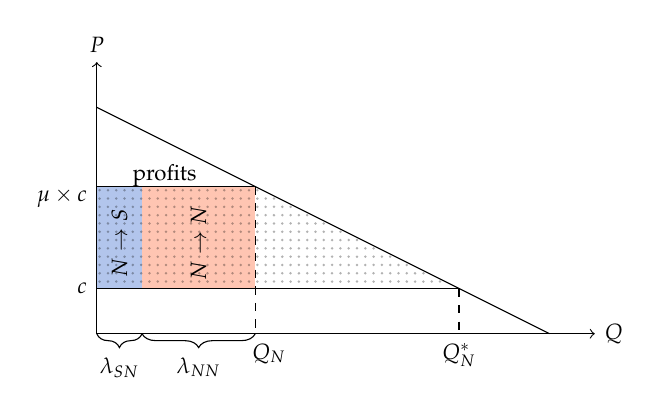
\begin{tikzpicture}[scale=0.575, every node/.style={font=\footnotesize}] 
\draw[->] (0,0) -- (11,0) node[right] {$Q$}; 
\draw[->] (0,0) -- (0,6) node[above] {$P$}; 
\draw (0,5) -- (10,0); 
\draw[dashed] (3.5,3.25) -- (3.5,0) node[below] {$\ \ \ \ \ Q_{N}$};       
 \draw[dashed] (8,1) -- (8,0) node[below] {$Q_{N}^{*}$};  
\draw (0,1) -- (8,1); 
\draw (0,3.25) -- (3.5,3.25); % Color the rectangle 
\fill[blue!50!teal, fill opacity=0.3] (0,1) rectangle (1,3.25); % Color the triangle 
\fill[red!50!orange, fill opacity=0.3] (1,1) rectangle (3.5,3.25); % Color the triangle 
%\fill[blue!30, fill opacity=0.3] (4,1) -- (3.5,3.25) -- (8,1) -- cycle; % Color the trapezoid 
\fill[pattern=dots, fill opacity=0.3] (0,1) -- (0,3.25) -- (3.5,3.25) -- (8,1) -- cycle; 
\node at (5.25,1.75) {};
\node at (1.5, 3.5) {profits};
\node[rotate=90] at (0.5,2) {$N \rightarrow S$};
\node[rotate=90] at (2.25,2) {$N \rightarrow N$};
\node[left] at (0,3) {$\mu \times c$}; 
\node[left] at (0,1) {$c$}; 
% Add braces and labels for Q_A and Q_B 
\draw[decorate, decoration={brace, amplitude=5pt, mirror}] (0,0) -- (1,0) node[midway, below=5pt] {$\lambda_{SN}$}; 
\draw[decorate, decoration={brace, amplitude=5pt, mirror}] (1,0) -- (3.5,0) node[midway, below=5pt] {$\lambda_{NN}$};

% Legend               
%\node[anchor=north west, font=\small] at (3,6) {             
%\begin{tabular}{c@{\hspace{0.2em}}l}                 
%\tikz\draw[fill=white, pattern=dots] (0,0) rectangle (0.85,0.3); & $\Delta Consumer \ Surplus$            
%\end{tabular}        
%}; 

\end{tikzpicture}    
\caption*{\large Country N} 
\end{subfigure}
\par\end{centering}
\vspace{-7.5pt}
\noindent\begin{minipage}[t]{1\columnwidth}%
\begin{spacing}{0.75}
{\footnotesize\emph{Note}}{\footnotesize : This figure describes the
welfare effects of markup wedges in a two-country and two-sector economy.
Firms charge a constant markup $\mu$ over marginal cost $\text{MC}$
in the sector for which demand and supply curves are displayed. The
other sector is efficient, with goods priced at marginal cost. $Q_{ii'}$
denotes the quantity of markup-distorted goods produced in location
$i$ and sold to location $i'$. $Q_{i}^{*}$ denotes the efficient
quantity of consumption in location $i$.}
\end{spacing}
%
\end{minipage}
\end{figure}

\medskip{}
Now, consider an open economy setting. Here, the textbook argument
breaks down because excess profits are no longer remitted within the
same location where they distort prices and reduce consumer surplus.
To illustrate this, we retain the assumption that consumer have access
to measure $M_{i}\equiv\mid\Omega_{i}\mid=1$ of varieties. However,
they now can choose from domestic and foreign varieties. In particular,
$\Omega_{i}=\Omega_{Ni}\cup\Omega_{Si}$ with $M_{Ni}\equiv\mid\Omega_{Ni}\mid$
and $M_{Si}\equiv\mid\Omega_{Si}\mid$. Since the total number of
varieties is unchanged (i.e., $M_{i}=1$) the price index of the differentiated
good is unaffected: $P=\mu\times c$. However, now a share $\lambda_{\ell i}=M_{\ell i}/M_{i}\coloneqq M_{\ell i}$
of country $i$'s demand quantity and expenditure comes from firms
located in country $\ell\in\{N,S\}$. 

Consider a scenario where $N$ has a revealed comparative advantage
in the differentiated sector, due to hosting a larger measure of differentiated
firms:
\[
M_{NS}>M_{SN}\quad\Longrightarrow\quad\lambda_{NS}>\lambda_{SN}
\]
The south $S$ is, thus, a net importer of the differentiated good
and a net exporter of the homogeneous good for markets to clear. 

The bottom panel in Figure \ref{fig: Textbook} illustrates the welfare
effects of markup pricing in the open economy scenario. Suppose profits
earned by firms located in country $i$ are repatriated to households
in that country. The loss to consumer surplus in country $i$ is now
offset by profits earned on both domestic and foreign sales. This
leads to a locational decoupling between profit rebates and the loss
to consumer surplus. Consequently, the welfare loss from markups no
longer equals the Harberger triangle. Instead, the losses are either
greater or smaller depending on whether country $i$ is a net payer
or recipient of excess profits to/from abroad. In this example, the
aggregate loss is amplified for the South ($S$) due to net profit
outflows. In particular, noting that $Q\coloneqq Q_{S}=Q_{N}$ under
symmetric demand, we get
\[
\mathscr{D}_{S}\ =\ \mathscr{D}_{S}^{(closed)}+\underbrace{\frac{\mu-1}{\mu}PQ\left(\lambda_{NS}-\lambda_{SN}\right)}_{\text{net profit outflows from \ensuremath{S}}}\ >\ \mathscr{D}_{S}^{(closed)}
\]
By comparison, the aggregate loss for the North ($N$) is attenuated
by net profit inflows from the South:
\[
\mathscr{D}_{N}\ =\ \mathscr{D}_{N}^{(closed)}-\underbrace{\frac{\mu-1}{\mu}PQ\left(\lambda_{NS}-\lambda_{SN}\right)}_{\text{net profit inflows to \ensuremath{N}}}\ <\ \mathscr{D}_{N}^{(closed)}.
\]
Profit-shifting effects, thus, constitute a pure distributive externality.
They are zero-sum transfers from one country to another, enabled by
inefficient price wedges. 

This stylized model clarifies that countries capturing a disproportionate
share of global excess profits benefit from profit-shifting externalities.
Appendix \ref{sec:Motivating-Evidence} presents stylized evidence
indicating that high-income countries indeed appropriate a larger
share of global excess profits. To conduct formal measurement, we
first formalize this mechanism in a general equilibrium model with
many countries and sectors operating under variable and heterogeneous
markups. We then show that markups operate as shadow tariffs when
countries are sufficiently open.

\section{\label{sec: Baseline Model}Theoretical Model}

We consider a semi-parametric model of the global economy consisting
of multiple countries, indexed by $n,\,i=1,..,N$. The product space
is partitioned into multiple industries, indexed by $k,g=1,...,K$.
Country $i$ hosts a fixed number of firms indexed by $\omega$ in
each industry $k$. Each firm supplies a single traded and differentiated
product variety. Labor is the only primary factor of production, and
each country $i$ is endowed with an inelastic supply of labor, $L_{i}$,
that is paid an equilibrium wage, $w_{i}$. Labor is internationally
immobile but mobile across different production activities within
a country.

\paragraph*{Demand.}

The representative consumer in country $n$ maximizes a semi-parametric
utility function with unitary elasticity of substitution across industries.
Let $\Omega_{n,k}$ denote the set of varieties available to the consumer
in industry $k$, with $\textbf{p}_{n,k}\equiv\{p_{\omega}\}_{\omega\in\Omega_{n,k}}$
denoting the price vector associated with these varieties. The demand
for individual varieties is of the \emph{homothetic with aggregator}
form, nesting an important class of demand systems commonly used in
the literature. Specifically, the share of expenditure on variety
$\omega\in\Omega_{n,k}$ with price $p_{\omega}$ is
\[
\lambda_{\omega}=\frac{\frac{p_{\omega}}{P_{n,k}}D_{k}(\frac{p_{\omega}}{P_{n,k}})}{\int_{\Omega_{n,k}}\frac{p_{\omega'}}{P_{n,k}}D_{k}(\frac{p_{\omega'}}{P_{n,k}})d\omega'},\qquad\qquad\left(\omega\in\Omega_{n,k}\right)
\]
where $P_{n,k}\equiv\mathscr{P}_{k}(\textbf{p}_{n,k})$ is a homogeneous
of degree one price aggregator. This aggregator solves the following
depending on whether preferences are directly implicit additive, indirectly
implicit additive, or of the single aggregator type (e.g., Kimball):
\[
1=\begin{cases}
\int_{\Omega_{n,k}}\int_{0}^{D(p_{\omega}/P_{n,k})}D_{k}^{-1}(x)dx\,d\omega & \left[\text{directly implicit additive}\right]\\
\\\int_{\Omega_{n,k}}\int_{0}^{p_{\omega}/P_{n,k}}D_{k}(x)dx\,d\omega & \left[\text{indirectly implicit additive}\right]\\
\\\int_{\Omega_{n,k}}\frac{p_{\omega'}}{P_{n,k}}D_{k}(p_{\omega'}/P_{n,k})d\omega & \left[\text{single aggregator}\right]
\end{cases}
\]
The function $D_{k}(x)$ is positive-valued and decreasing over $x\in\left(0,a\right)$
and exhibits a constant \emph{relative} choke price $a\in\mathbb{R}_{+}$:
$\lim_{x\rightarrow a}D_{k}\left(x\right)=0$ and $D_{k}\left(x\right)=0$
for $x\geq a$. Without loss of generality we normalize $a=1$, hereafter.\medskip{}

\noindent\emph{Demand Function}.$\quad$ The demand facing a firm
$\omega\in\Omega_{n,k}$ is fully determined by its price $p_{\omega}$,
two aggregate shifters, $P_{n,k}$ and $\Upsilon_{n,k}$. Namely,
\[
q_{\omega}\,=\,q_{k}(p_{\omega};\,P_{n,k},\Upsilon_{n,k})\equiv D_{k}(p_{\omega}/P_{n,k})\Upsilon_{n,k}
\]
where $P_{n,k}$ is the price aggregator defined above and $\Upsilon_{n,k}\equiv\frac{e_{n,k}E_{n}}{P_{n,k}}\left(\int_{\Omega_{n,k}}\frac{p_{\omega'}}{P_{n,k}}D_{k}(\frac{p_{\omega'}}{P_{n,k}})d\omega'\right)^{-1}$,
with $e_{n,k}$ denoting the constant share of expenditure on industry
$k$ goods and $E_{n}$ denoting total expenditure in country $n$.

\paragraph*{Firms and Production.}

Country $i$ hosts a fixed set of firms in industry $k$ that sell
to various locations and compete under monopolistic competition. In
our baseline model, there are no fixed overhead costs associated with
accessing individual markets. Hence, firm selection across markets
is driven solely through the choke price. Throughout the paper, we
assume that goods markets are perfectly segmented across countries.
Let $\Omega_{in,k}\subset\Omega_{i,k}$ denote the set of firms that
actively serve market $n$ from origin $i$. For firm $\omega\in\Omega_{in,k}$
with productivity $\varphi$, the unit cost of supplying its variety
to country $n$ is,
\[
c_{\omega}=\frac{w_{i}\tau_{in,k}}{\varphi_{\omega}},\qquad\qquad\omega\in\Omega_{in,k}
\]
where $\tau_{in}\geq1$ represents the iceberg trade cost (with $\tau_{ii}=1$)
and $w_{i}$ is the wage rate.\medskip{}

\noindent \emph{Firm Productivity Distribution}.$\quad$The firm-level
productivity $\varphi$ is the realization of a random variable drawn
independently across firms in each country and industry from distribution
$G_{i,k}(\varphi)$. As in \citet{melitz2008market}, we assume that
$G_{i,k}$ is Pareto with a location-specific scale parameter but
the same shape parameter $\theta>0$ globally, with $\varphi\geq\bar{\varphi}_{i,k}$:
\begin{equation}
G_{i,k}\left(\varphi\right)=1-\left(\bar{\varphi}_{i,k}/\varphi\right)^{\theta}.\label{eq:Pareto Distibution}
\end{equation}

\medskip{}

\noindent \emph{Profit Maximization and Markups}.$\quad$The profits
collected by firm $\omega\in\Omega_{in,k}$ from sales to market $n$
can be specified as
\[
\pi_{k}(p_{\omega};\,c_{\omega},P_{n,k},\Upsilon_{n,k})=\left(p_{\omega}-c_{\omega}\right)q_{k}(p_{\omega};\,P_{n,k},\Upsilon_{n,k})
\]
The firms are monopolistically competitive and choose their price
$p_{\omega}$ \`a la Bertrand to maximize profits. Firms' profit
maximization implies an optimal price that exhibits a variable and
heterogeneous markup $\mu_{\omega}$ over marginal cost:
\[
p_{\omega}=\mu_{\omega}\times c_{\omega}
\]
where $\mu_{\omega}=m_{k}(\nu_{\omega})$, with $\nu_{\omega}\equiv P_{n,k}/c_{\omega}$
representing the competitiveness of variety $\omega\in\Omega_{in,k}$
in that market. The function $m_{k}(\nu_{\omega})$ is injective and
the implicit solution to
\[
m_{k}(\nu_{\omega})=\frac{\varepsilon_{k}(\frac{m_{k}(\nu_{\omega})}{\nu_{\omega}})}{\varepsilon_{k}(\frac{m_{k}(\nu_{\omega})}{\nu_{\omega}})-1},
\]
where $\varepsilon_{k}(x)\equiv-\partial\ln D_{k}(x)/\partial\ln x$.
We assume that $\varepsilon_{k}'(x)<0$, which is a sufficient condition
for $m_{k}(.)$ to be injective. Since $\lim_{x\to1}\varepsilon_{k}(x)=\infty$,
then $m_{k}(1)=1$, indicating that the marginal cost $c$ of the
least efficient firm that can remain active is equal to the choke
price, irrespective of the firm's origin. Accordingly, firms actively
selling from origin $i$ to destination $n$, have $\nu$ values that
span the entire set $\mathcal{V}=[1,\infty]$, irrespective of the
cost and demand profiles of countries $i$ and $n$.

\paragraph*{General Equilibrium.}

For a given set of parameters, equilibrium is vector of demand quantities,
$\textbf{q}$, prices, $\textbf{p}$, wages, $\textbf{w}$, and income,
$\textbf{Y}$, such that the representative consumer's utility is
maximized in each country; firm-level profits are maximized; labor
markets clear, so wage payments in country $i$ equal sales net of
markups,
\[
w_{i}L_{i}=\sum_{n=1}^{N}\sum_{k=1}^{K}\left[\int_{\Omega_{in,k}}\frac{1}{\mu_{\omega}}p_{\omega}q_{\omega}d\omega\right];
\]
and aggregate expenditure $E_{i}$ equals aggregate income, $Y_{i}$,
which is wage income plus lump-sum profit rebates:
\begin{equation}
E_{i}=Y_{i}=w_{i}L_{i}+\underbrace{\sum_{n=1}^{N}\sum_{k=1}^{K}\left[\int_{\Omega_{in,k}}\left(1-\frac{1}{\mu_{\omega}}\right)p_{\omega}q_{\omega}d\omega\right]}_{\text{profits}}.\label{eq: E=00003DY (eq)}
\end{equation}
Our baseline model assumes that profits are entirely rebated to consumers
in the firms' country of origin. Later, we relax this assumption and
allow for multinational production and global profit ownership.

\medskip{}

\noindent \emph{Aggregate equilibrium shares}.$\quad$ Aggregate
trade shares are described by a gravity equation
\[
\lambda_{in,k}=\frac{\chi_{i,k}(\tau_{in,k}w_{i})^{-\theta}}{\sum_{\ell}\chi_{\ell,k}(\tau_{\ell n,k}w_{\ell})^{-\theta}},
\]
with a trade elasticity equal to $\theta$ . The shifter $\chi_{i,k}$
collects all the constants, including those specific to ($i,k$),
such as $\bar{\varphi}_{i,k}$. Total sales from country $i$ are
thus $Y_{i}=\sum_{n}\sum_{k'}\lambda_{in,k'}e_{n,k'}E_{n}$, where
$e_{n,k}$ is the constant expenditure share on industry $k$ in destination
$n$ Accordingly, the share of country $i$'s sales collected from
goods pertaining to industry $k$ is
\begin{equation}
y_{i,k}=\frac{\sum_{n}\lambda_{in,k}e_{n,k}E_{n}}{\sum_{n}\sum_{k'}\lambda_{in,k'}e_{n,k'}E_{n}}.\label{eq: y_ik}
\end{equation}


\paragraph*{Markup-Based Equilibrium Representation.}

Recall that for each country-pair the set of firms that actively export
from one to the other spans the entire set $\nu\in(1,\infty)$. Hence,
it is straightforward to verify that the markup distribution of exports
from any origin to any destination has a common form:
\[
\widetilde{G}_{in,k}(\mu)=\widetilde{G}_{k}(\mu)\equiv\text{Pr}\left\{ m_{k}(\nu)\leq\mu\;\mid\ \nu\geq1\right\} 
\]
 Since $m_{k}(.)$ is injective and firm productivity, and thus, $\nu$,
follows a Pareto distribution, the markup distribution can be obtained
as
\[
\widetilde{G}_{k}(\mu)=1-\left(m_{k}^{-1}(\mu)\right)^{-\theta}.
\]
Additionally, within industry $k$, there is a one-to-one country-blind
correspondence between a firm's markup and its competitiveness measure,
$\nu_{k}(\mu)=m_{k}^{-1}(\mu)$. As a result, for any market $n$,
the price is fully determined by knowing the markup as
\[
p_{n,k}(\mu)=\frac{\mu}{m_{k}^{-1}(\mu)}P_{n,k}
\]
Note that the origin-specific cost shifters ($\tau$ and $w$) do
not explicitly appear in the above equation, but they implicitly influence
the markup $\mu$. Firms from higher cost locations charge a lower
markup with the same productivity, which also translates to a lower
$m_{k}^{-1}(\mu)$. In other words, firm markups convey all the price-relevant
information marginal cost parameters.

Building on these observations, for any market $n$, the market share
of firms with markup $\mu$ within industry $k$ is given by
\[
\lambda_{k}\left(\mu\right)=\frac{\frac{\mu}{m_{k}^{-1}(\mu)}D_{k}(\frac{\mu}{m_{k}^{-1}(\mu)})\widetilde{g}_{k}(\mu)}{\int_{1}^{\infty}\frac{x}{m_{k}^{-1}(x)}D_{k}(\frac{x}{m_{k}^{-1}(x)})\widetilde{g}_{k}(x)dx}
\]
irrespective of its origin, where $\widetilde{g}_{k}(x)\equiv d\widetilde{G}_{k}(x)/dx$.
Note that $\lambda_{k}(\mu)$ is not only origin blind but it is also
destination-blind, since the aggregator $P_{n,k}$ shifts all prices
in market $n$ uniformly without affecting relative demand shares;
thus, dropping out of the above equation.\medskip{}

\noindent \emph{Aggregate expenditure and sales shares}.$\quad$Country
$i$'s aggregate share of expenditure on goods with markup $\mu\in[1,\infty)$
is the weighted sum across all industries 
\[
e_{i}(\mu)=\sum_{k}e_{i,k}\lambda_{k}(\mu),
\]
where $e_{i,k}$ is the industry-level expenditure share pinned down
by the cross-industry utility aggregator and the aggregate sales shares
are 

\[
y_{i}(\mu)=\sum_{k}y_{i,k}\lambda_{k}(\mu)
\]
where $y_{i,k}$ is the industry-level sales share described by Equation
\ref{eq: y_ik}. These equations draw on the result that $\lambda_{k}(\mu)$
is independent of destination and origin, representing the within-industry
share of expenditure and sales for varieties with markup $\mu$.

\paragraph*{Additional Notation.}

To condense the notation, we hereafter use $\mathbb{E}_{\omega}\left[.\right]$,
$\widetilde{\mathbb{E}}_{\omega}\left[.\right]$, and $MLD_{\omega}\left[.\right]$
to denote the \emph{arithmetic mean}, \emph{harmonic} \emph{mean,
}and \emph{mean log deviation }operators. In particular, for a generic
function, $f:[1,\infty)\rightarrow\mathbb{R}$, define
\begin{align*}
\mathbb{E}_{\omega}\left[f\left(\mu\right)\right]\equiv\int_{1}^{\infty}f\left(\mu\right)\omega\left(\mu\right)d\mu & \qquad\qquad\left(\text{Arithmetic mean}\right)\\
\\\widetilde{\mathbb{E}}_{\omega}\left[f\left(\mu\right)\right]\equiv\left(\int_{1}^{\infty}f\left(\mu\right)^{-1}\omega\left(\mu\right)d\mu\right)^{-1} & \qquad\qquad\left(\text{Harmonic mean}\right)\\
\\MLD_{\omega}\left[f(\mu)\right]=\ln\mathbb{E}_{\omega}\left[f(\mu)\right]-\mathbb{E}_{\omega}\left[\ln f(\mu)\right] & \qquad\qquad\left(\text{Mean log deviation}\right)
\end{align*}
where $\omega:[1,\infty)\rightarrow[0,1]$ is a well-behaved weight
function that satisfies $\int_{1}^{\infty}\omega\left(\mu\right)d\mu=1$.
To showcase how the above operators simplify notation, take the aggregate
expendable income described by Equation \ref{eq: E=00003DY (eq)}.
Appealing to our definition for sales share, $y_{i}(\mu)$, we can
rewrite this equation as
\[
Y_{i}=w_{i}L_{i}+\left[\int_{1}^{\infty}\left(1-\frac{1}{\mu}\right)y_{i}(\mu)d\mu\right]Y_{i}
\]
Rearranging this equation yields a more compact expression for aggregate
income:
\[
Y_{i}=\left[\int_{1}^{\infty}\frac{1}{\mu}y_{i}(\mu)d\mu\right]^{-1}w_{i}L_{i}\,=\,\widetilde{\mathbb{E}}_{y_{i}}\left[\mu\right]w_{i}L_{i},
\]
where $\widetilde{\mathbb{E}}_{y_{i}}\left[\mu\right]$ is country
$i$'s output-weighted harmonic mean markup.

\section{\label{sec: Cost of Markups}Aggregate Welfare Loss from Market Power}

The market equilibrium is inefficient, because markups cause relative
prices (relative marginal rates of substitution) to diverge from relative
marginal costs (relative marginal rates of transformation). More formally,
\[
\frac{p_{\omega}}{p_{\omega'}}\ =\ \frac{\mu_{\omega}}{\mu_{\omega'}}\,\frac{c_{\omega}}{c_{\omega'}}\ \neq\ \frac{c_{\omega}}{c_{\omega'}}.
\]
Our goal is to measure the aggregate welfare loss from market power.
To this end, we begin a formal definition of aggregate welfare in
our economic setting.\medskip{}
\\
\noindent\emph{\uline{Aggregate welfare}}\uline{.}$\quad$We define
aggregate welfare as the utility of the representative consumer. We
can specify this measure for country $i$ under the factual markups
$\boldsymbol{\mu}$ as
\[
W_{i}(\textbf{\ensuremath{\boldsymbol{\mu}}};\boldsymbol{\tau})=v_{i}(E_{i},\textbf{p}_{i}),
\]
where $v_{i}(.)$ is the indirect utility function. $E_{i}=\widetilde{\mathbb{E}}_{y_{i}}\left[\mu\right]w_{i}L_{i}$
denotes expendable income under the status quo, which is the sum of
wage income and profit rebates. $\textbf{p}_{i}=\{p_{\omega}\}_{\Omega_{i}}$
is the equilibrium vector of prices in country $i$, where $p_{\omega}=\mu_{\omega}c_{\omega}$.

Now, consider a counterfactual equilibrium in which markups are eliminated.
This would yield an efficient allocation wherein prices are equal
to marginal cost globally: $\textbf{p}^{*}=\textbf{c}^{*}\equiv\{c_{\omega}^{*}\}_{\Omega^{*}}$.
Total expendable income equals merely the wage income, $E_{i}^{*}=w_{i}^{*}L_{i}$,
after this shift. Eliminating markups, modifies the entire vector
of wages and, thus, marginal costs, with $w^{*}$ and $c^{*}$ denoting
the wage and marginal cost under the efficient equilibrium. Welfare
under the efficient marginal-cost-pricing allocation is
\[
W_{i}(\textbf{\ensuremath{\boldsymbol{1}}};\boldsymbol{\tau})=v_{i}(E_{i}^{*},\textbf{p}_{i}^{*}).
\]
\\
\noindent\emph{\uline{Aggregate welfare loss from market power}}\uline{.}$\quad$We
define the welfare loss from market power for country $i$ as the
log welfare distance to the efficient marginal-cost-pricing equilibrium:
\[
\mathscr{D}_{i}(\boldsymbol{\tau})\equiv\Delta_{\mu}\ln W_{i}=\ln W_{i}(\textbf{1};\boldsymbol{\tau})-\ln W_{i}(\boldsymbol{\mu};\boldsymbol{\tau}).
\]
It is important to reiterate that the marginal-cost-pricing equilibrium
\emph{without} transfers represents one point on the Pareto efficient
frontier. As show in Appendix \ref{sec: Proof Lemma 1} this allocation
can be rationalized as the solution to a global planning problem under
a specific choice of Pareto weights. However, as we will later demonstrate,
some countries could be worse off after transitioning from the status
quo to marginal-cost-pricing equilibrium, though the weighted sum
of global welfare improves. 

\subsection{Closed Economy Setting}

As an intermediate step, we analyze a closed economy setting. This
setting is characterized by prohibitively high trade costs ($\boldsymbol{\tau}\rightarrow\infty$)
implying equality between domestic output and expenditure: $\lambda_{ii}=1$
and $\textbf{y}_{i}=\textbf{e}_{i}$. The following proposition shows
that the aggregate loss from markups in this setting is purely determined
by markup dispersion.
\begin{prop}
The aggregate welfare loss from market power for a closed economy
is
\[
\mathscr{D}_{i}(\boldsymbol{\tau}\rightarrow\infty)=\ \text{MLD}_{e_{i}}\left[1/\mu\right]\ \simeq\ \frac{1}{2}\text{Var}_{e_{i}}\left[\ln\mu\right]
\]
where $\text{MLD}_{e_{i}}[\frac{1}{\mu}]=\ln\mathbb{E}_{e_{i}}[\frac{1}{\mu}]-\mathbb{E}_{e_{i}}[\ln\frac{1}{\mu}]$
is the mean log deviation of inverse markups, which is an entropy-based
measure of markup dispersion.
\end{prop}
The above formula generalizes the \citet{hsieh2009misallocation}
formula to a setting endogenous wedges and firm selection effects.
It reflects the logic outlined earlier. The inefficiency arising from
market power stems from the divergence between relative prices and
relative marginal costs. If markups are uniform, they preserve the
equality between relative prices and relative marginal costs and,
therefore, do not disrupt allocative efficiency---even if they are
nonzero.

\subsection{Open Economy Setting}

Now consider an open economy for which supply and demand are decoupled,
$\textbf{y}_{i}\neq\textbf{e}_{i}$, and the domestic expenditure
share is strictly less than one, $\lambda_{ii}<1$, and endogenously
determined. We derive a new formula for the welfare loss from market
power in this case. 
\begin{prop}
The aggregate welfare loss from market power for an open economy is
\begin{equation}
\mathscr{D}_{i}(\boldsymbol{\tau})=\ \underbrace{\text{MLD}_{e_{i}}\left[1/\mu\right]}_{\text{markup dispersion}}\ +\ \underbrace{\ \frac{1}{\theta}\,\Delta_{\mu}\ln\tilde{\lambda}_{ii}\ }_{\Delta\text{gains from trade}}\ +\underbrace{\ \ln(\widetilde{\mathbb{E}}_{e_{i}}\left[\mu\right]/\widetilde{\mathbb{E}}_{y_{i}}\left[\mu\right])}_{\text{ profit shifting}}\label{eq: D_i Open Economy}
\end{equation}
where $\Delta_{\mu}\ln\tilde{\lambda}_{ii}\equiv\sum_{k}e_{i,k}\Delta_{\mu}\ln\lambda_{ii,k}$
is a geometric mean of markup-induced change in domestic expenditure
share and the profit shifting effects are internationally zero-sum
constituting a pure distributive externality: $\ln\sum_{i}\frac{w_{i}\,L_{i}}{w\cdot L}\,(\widetilde{\mathbb{E}}_{y_{i}}\left[\mu\right]/\widetilde{\mathbb{E}}_{e_{i}}\left[\mu\right])=0.$
\end{prop}
The aggregate welfare loss has three elements under trade relations.
The first element, $\text{MLD}_{e_{i}}\left[1/\mu\right]$, mirrors
the closed economy formula. The second terms captures how markup correction
affects the gains from trade. These gains depend on the extent to
which markup correction modifies relative international expenditure
shares, $\Delta_{\mu}\ln\tilde{\lambda}_{ii}=\ln\tilde{\lambda}_{ii}(\boldsymbol{\mu};\boldsymbol{\tau})-\ln\tilde{\lambda}_{ii}(\boldsymbol{1};\boldsymbol{\tau})$.
And since the within-industry markup distribution is origin-blind,
expenditure share changes arise exclusively from shifts in relative
wages, which are muted as we confirm quantitatively in later analysis.\footnote{Formally: $\Delta_{\mu}\ln\tilde{\lambda}_{ii}=\int_{\boldsymbol{\mu}}^{1}\left(\frac{\partial\ln\tilde{\lambda}_{ii}}{\partial\ln\textbf{w}}\cdot\frac{\partial\ln\textbf{w}}{\partial\boldsymbol{\mu}}d\boldsymbol{\mu}\right)$,
where $\frac{\partial\ln\textbf{w}}{\partial\boldsymbol{\mu}}$ is
the wage change in response to markup correction and partial derivative
in the integral is $\frac{\partial\ln\tilde{\lambda}_{ii}}{\partial\ln\textbf{w}}\cdot\frac{\partial\ln\textbf{w}}{\partial\boldsymbol{\mu}}=\theta\left[-(1-\tilde{\lambda}_{ii})\frac{\partial\ln w_{i}}{\partial\boldsymbol{\mu}}+\boldsymbol{\tilde{\lambda}}_{-ii}\cdot\frac{\partial\ln\boldsymbol{w}_{-i}}{\partial\boldsymbol{\mu}}\right].$} Also, this terms is fundamentally distributive: if markups depress
relative wages in one group of countries, they inevitably elevate
them in others. Thus, $\Delta_{\mu}\ln\tilde{\lambda}_{ii}$ becomes
positive for the former and negative for the latter.

The last term, which represents rent-shifting is the most notable,
and largely overlooked by the past literature. To understand the intuition,
let us first refer back to the closed economy case: there, profits
were rebated to the same consumers whose surplus was negatively impacted
by markups. Now, markup could undermine consumer surplus in one location,
generating excess profits that are rebated elsewhere. Hence, the loss
from market power is elevated or mitigated, depending on whether country
$i$ is a net receiver or a net payer of excess profits to the rest
of the world. Consistent with this logic, exposure to profits-shifting
effects is determined by a country's revealed comparative advantage
across low versus high-markup goods. Specifically,
\[
\ln(\widetilde{\mathbb{E}}_{e_{i}}\left[\mu\right]/\widetilde{\mathbb{E}}_{y_{i}}\left[\mu\right])\,\approx\,\widetilde{\mathbb{E}}_{e_{i}}\left[\mu\right]\times Cov\left(\frac{y_{i}(\mu)}{e_{i}(\mu)},\frac{1}{\mu}\right),
\]
where $Cov\left(.\right)$ is the covariance operator. The above equation
states that a country's exposure to profit-shifting externalities
is regulated by its pattern of specialization. Positive exposure results
from revealed comparative advantage in high-markup goods, i.e., $\partial(\frac{y_{i}(\mu)}{e_{i}(\mu)})/\partial\mu>0$.
And negative exposure stems from revealed comparative advantage in
low-markup goods.

\emph{\medskip{}
}

\noindent\emph{\uline{Does trade openness impact the loss}}\emph{?}$\quad$We
define the pure effect of trade as the change relative to the no trade
of autarky benchmark. Specifically, for a generic variable $X$ define
the trade-induced change as
\[
\Delta_{\tau}X\equiv X(\boldsymbol{\tau})-X(\boldsymbol{\infty}),
\]
where $X(\boldsymbol{\tau})$ denotes the value of $X$ under the
status quo trade cost levels and $X(\boldsymbol{\infty})$ denotes
the counterfactual level under prohibitive trade costs or autarky. 

Our goal is to determine $\Delta_{\tau}\mathscr{D}_{i}^{\mu}$ using
the formulas under Propositions 1 and 2. The markup dispersion term
in these formulas is invariant to trade, given our previous result
that the markup distribution, $\widetilde{G}_{k}(\mu)$, and the conditional
expenditure share, $\lambda_{k}(\mu)$, is unaffected by trade costs.
The intuition for this invariance is that the pro-competitive effects
of on markups at the intensive margin are exactly offset by the selection
effects at the extensive margin. Thus, the degree of markup dispersion
is unaffected by trade \emph{within} narrowly-defined industry segments,
i.e., $\Delta_{\tau}\text{MLD}_{e_{i}}\left[1/\mu\right]=0$. 

Instead, trade openness influences the welfare loss from market power
in two ways. First, market power distorts international relative prices
and the gains from trade in open economies. Second, trade activates
the zero-sum profit shifting effects discussed earlier. Formally,
the pure effect of trade is
\[
\Delta_{\tau}\mathscr{D}_{i}=\ \frac{1}{\theta}\,\Delta_{\mu}\ln\tilde{\lambda}_{ii}\ +\ \ln(\widetilde{\mathbb{E}}_{e_{i}}\left[\mu\right]/\widetilde{\mathbb{E}}_{y_{i}}\left[\mu\right]).
\]
The first term represents the change to the efficiency gains from
trade relative to what the gains would have been without markup distortions.
The second represents profit-shifting effects.

\emph{\medskip{}
}

\noindent\emph{\uline{The Gains from Trade}}\emph{.}$\quad$While
profit-shifting externalities attenuate the gains from trade for some
countries, they do not reverse the overall benefits of trade. This
point can be formalized using the standard definition of the gains
from trade, $GT_{i}=1-W_{i}(\boldsymbol{\mu};\boldsymbol{\infty})/W_{i}(\boldsymbol{\mu};\boldsymbol{\tau})$.
These gains are described by the following formula:
\[
GT_{i}=1-\Lambda_{i}\,\tilde{\lambda}_{ii}^{\frac{1}{\theta}},\qquad with\qquad\Lambda_{i}\equiv\frac{\widetilde{\mathbb{E}}_{e_{i}}\left[\mu\right]}{\widetilde{\mathbb{E}}_{y_{i}}\left[\mu\right]}
\]
where $\Lambda_{i}$ represents profit-shifting effects specified
by Proposition 2 and $\tilde{\lambda}_{ii}^{\frac{1}{\theta}}$ denotes
the efficiency gains, where $\tilde{\lambda}_{ii}\equiv\prod_{k}\lambda_{ii,k}^{e_{i,k}}$
is the geometric mean of domestic expenditure shares across industries.
Overall, the above formula suggests that profit-shifting magnifies
the gains from trade for countries that collect net profits from the
rest of the world while diminishing them for others. In principle,
rent-shifting effects could large enough to reverse the gains from
trade. However, outside of extreme cases, the overall gains should
remain positive if $\theta$ is sufficiently low. 

\subsection{\label{sec: Extensions}Extensions}

We re-derive the formula for $\mathscr{D}_{i}$ and $\Delta_{\tau}\mathscr{D}{}_{i}$
under free entry, multi-national ownership, input-output linkages,
and fixed overhead costs. In the interest of brevity we present a
verbal description of each extension here, with detailed derivations
provided in the appendix.

\paragraph{$\left(a\right)$ Free Entry and Rent Dissipation.}

Our baseline model abstracts from firm entry and the fact that a fraction
of profits represents quasi-rents used to cover sunk entry costs.
Appendix \ref{sec: Misallocation Free Entry} demonstrates that even
with firm entry, cross-country profit imbalances generate distributive
firm-relocation externalities that mirror the profit-shifting effects
identified earlier. These relocation externalities, however, arise
not from excessive markups but rather from excessive entry of firms
into low-markup industries.

Specifically, suppose firms pay a sunk entry cost to develop a blueprint.
The number of entrants paying this cost is determined by a free-entry
condition that equates variable profits to the entry cost in each
industry and country. For simplicity, assume demand exhibits a CES
parametrization. We show that a closed economy's distance to the efficient
frontier under free entry is
\[
\mathscr{D}_{i}^{closed}=\mathbb{E}_{e_{i}}\left[\mu\ln\mu\right]-\mathbb{E}_{e_{i}}\left[\mu\right]\ln\mathbb{E}_{e_{i}}\left[\mu\right].
\]
This formula represents the aggregate welfare loss from inefficient
firm entry decisions, which fail to internalize the social benefits
of adding new product varieties. The extent of this loss is tied to
the degree of markup dispersion: $\mathscr{D}_{i}^{closed}\approx Var_{e_{i}}[\mu]$.
Trade openness modifies welfare losses through firm-relocation externalities.
As demonstrated in Appendix section \ref{sec: Misallocation Free Entry},
the trade-induced change in $\mathscr{D}_{i}$ is
\[
\Delta_{\tau}\mathscr{D}_{i}=\mathbb{E}_{e_{i}}\left[\left(\mu-1\right)\ln\frac{y_{i}^{*}\left(\mu\right)}{y_{i}\left(\mu\right)}\right],
\]
where $y_{i}^{*}\left(\mu\right)$ denotes the counterfactual output
share under the efficient allocation. One can verify that $y_{i}^{*}\left(\mu\right)/y_{i}\left(\mu\right)$
is increasing in $\mu$ if a country is a net exporter of high-markup
goods, implying that firm-delocation mitigates the loss from entry
distortions (\emph{i.e.}, $\Delta_{\tau}\mathscr{D}_{i}<0$) for the
same countries that benefit from profit-shifting.\footnote{The argument goes as follows: restoring efficiency entails increasing
the relative wage of countries that are net exporters of high-markup
goods. The higher wage suppresses demand relatively more for these
countries' output of low-markup goods, since these goods face more
price-elastic demand.} In other words, firm-delocation effects generate distributive externalities
that merely mirror profits-shifting effects.\footnote{Figure \ref{fig: free entry} in the appendix illustrates this point
by simulating a generic model featuring two countries. The countries
are symmetric except for their revealed comparative advantage in low-markup
versus high-markup goods. The simulation demonstrates that under both
free and restricted entry, trade openness amplifies the deadweight
loss of monopoly distortions for the country that is a net importer
of high-markup goods. Conversely, it reduces these costs for the other
country. This affirms that monopoly distortions have internationally
zero-sum effects, even in scenarios where firm entry dissipates quasi-rents.
The underlying logic is that the degree of market power is correlated
with entry distortions, and exposure to these distortions mirrors
exposure to profit-shifting under restricted entry.} 

\paragraph*{$\left(b\right)$ Multinational Ownership and Cross-Border Profit
Payments.}

As documented earlier, only a minor fraction of profits are repatriated
to foreign shareholders---hence, the abstraction from cross-border
profit payments in our baseline model. However, we can easily extend
our baseline formulas to account for such payments. Appendix \ref{sec: DWL multinational ownership}
derives updated formulas for $\Delta\mathscr{D}_{i}$, under the condition
where a constant share $\pi_{ni}$ of country $n$'s profits are repatriated
to international shareholders in country $i$. The new formula for
$\Delta\mathscr{D}_{i}$ features an additional term that accounts
for the cross-border profit payments to foreign shareholders. More
formally,\vspace{-10pt}
\begin{align}
\Delta_{\tau}\mathscr{D}_{i} & \ =\ \frac{1}{\theta}\,\Delta_{\mu}\ln\tilde{\lambda}_{ii}\ +\ \overbrace{\ln\left(\widetilde{\mathbb{E}}_{e_{i}}\left[\mu\right]/\widetilde{\mathbb{E}}_{y_{i}}\left[\mu\right]\right)}^{\text{gross profit-shifting}}\ \label{eq: delat_D (MN ownership)}\\
 & \ -\underbrace{\ln\left(1+\sum_{n\neq i}\left[\pi_{ni}\frac{Y_{n}}{Y_{i}}(1-\frac{1}{\mathbb{\widetilde{E}}_{y_{n}}[\mu]})-\pi_{in}(1-\frac{1}{\mathbb{\widetilde{E}}_{y_{i}}[\mu]})\right]\right)}_{\text{adjusting for multinational profit payments}}
\end{align}
The last term in the above equation represents the net inflow of repatriated
profits for country $i$, calculated as the difference between the
inflow and outflow of such profits. Importantly, the semi-parametric
model allows us to evaluate this term using aggregate profit ownership
shares, denoted as $\left\{ \pi_{ni}\right\} _{n,i}$, which can be
inferred from firm-level ownership data. The calculation also requires
data on industry-level output and expenditure shares and the sales-weighted
average markup for each industry, as in our baseline model.

\paragraph*{$\left(c\right)$ Global Input-Output Networks.}

Appendix \ref{sec: Appendix IO} examines a global economy in which
production relies on labor and internationally traded intermediate
inputs. In this extension, the magnitude of international profit-shifting
depends on the degree to which the markup paid on imported inputs
is re-exported and passed on to foreign consumers after production.
As a result, the formulas that describe the impacts of trade on the
national-level incidence of monopoly distortions depend on the elements
of the global input-output matrix. We present these sufficient statistics
formulas in Appendix \ref{sec: Appendix IO} and observe that the
core logic from our baseline model continues to hold. Specifically,
trade intensifies the incidence of monopoly distortions for countries
that are net exporters of high-markup goods while reducing it for
others, where net exports now take into account global input-output
linkages.

\paragraph*{$\left(d\right)$ \label{subsec: Firm-Selection}Accounting for Fixed
Overhead Costs.}

Earlier, we showed that considering \emph{sunk} entry cost payments
does not eliminate the zero-sum welfare effects associated with market
power. In Appendix \ref{sec:Proof P4}, we explore how accounting
for fixed overhead costs affects the zero-sum international profit-shifting
effects. Specifically, we analyze a global economy where serving individual
markets requires paying a fixed cost that consumes a portion of the
profits. We provide updated formulas for calculating the welfare loss
from market power, isolating how trade alters these costs. Our updated
formulas demonstrate that a country's exposure to international profit-shifting
in the presence of fixed overhead costs is influenced by two factors:
the shape of the firm productivity distribution and how this industry-specific
shape parameter correlates with a country's net exports. These factors
determine the net profits paid to the rest of the world via fixed
cost payments.

\section{\label{sec: Implications-for-Policy}Duality Between Tariffs and
Markups}

This section shows that, for sufficiently open economies, markups
function as a shadow tariff. The general idea is that both markups
and tariffs introduce a local efficiency loss to extract excess surplus
in the form of government revenues or profits from the rest of the
world. Both wedges, therefore, have similar aggregate welfare effects.
To formalize this point, we first define the general equilibrium under
tariffs and markups.\emph{\medskip{}
}

\noindent\emph{\uline{General Equilibrium with Tariffs.}}$\quad$Suppose
that the price of every variety $\omega\in\Omega_{i}$ available to
consumers in country $i$ includes an additional wedge that is applied
specifically to imported varieties:
\[
p_{\omega}=\begin{cases}
(1+t_{i})\,\mu_{\omega}\,c_{\omega} & \omega\in\Omega_{-ii}\\
\mu_{\omega}\,c_{\omega} & \omega\in\Omega_{ii}
\end{cases},
\]
We focus on uniform tariffs, as the optimal tariff is uniform absent
markup wedges. That is, the uniform tariff outperforms any heterogeneous
tariff schedule for country $i$, starting from the efficient-pricing
schedule.\footnote{The uniformity of optimal tariffs is a general result that holds across
a wide class of constant-returns to scale quantitative trade models,
in which labor is the only primary production factor and labor market
are non-segmented within countries.} Tariffs also generate revenues to the amount of $\frac{t_{i}}{1+t_{i}}(1-\lambda_{ii})E_{i}$,
where $(1-\lambda_{ii})E_{i}$ is total import expenditure. Total
expendable income inclusive of tariff revenues is
\[
E_{i}=\widetilde{\mathbb{E}}_{y_{i}}\left[\mu\right]w_{i}L_{i}+\frac{t_{i}}{1+t_{i}}(1-\lambda_{ii})E_{i}.
\]
where $\lambda_{ii}=\sum_{k}e_{i,k}\lambda_{ii,k}$ is the aggregate
domestic expenditure share, aggregate over all industries. The industry-level
aggregate expenditure shares are described by the gravity equation
adjusted for tariffs:
\[
\lambda_{ni,k}=\frac{\chi_{n,k}[\,(1+t_{i})^{\mathbb{1}_{n\neq i}}\,\tau_{ni,k}w_{n}]^{-\theta}}{\sum_{\ell}\chi_{\ell,k}[\,(1+t_{i})^{\mathbb{1}_{\ell\neq i}}\,\tau_{\ell i,k}w_{\ell}]^{-\theta}}
\]
Lastly, since the economy is plagued with additional distortive wedges,
we specify aggregate welfare as an explicit function of both markups
and tariffs: $W_{i}(\boldsymbol{\mu},\textbf{t};\boldsymbol{\tau})=v_{i}(E_{i},\textbf{p}_{i})$.
Let $\boldsymbol{\mu}_{i}\equiv\{\mu_{\omega}\}_{\cup_{n}\Omega_{in}}\subset\boldsymbol{\mu}$
denote the subset of markups applied by firms located in country $i$.
With a slight abuse of notation we hereafter use
\[
W_{i}(\boldsymbol{\mu}_{i},\textbf{t}_{i})\coloneqq W_{i}(\boldsymbol{\mu}_{i},\textbf{t}_{i};\boldsymbol{\mu}_{-i},\textbf{t}_{-i},\boldsymbol{\tau})
\]
 to denote welfare under a choice of local markups and tariffs given
markups and tariffs in the rest of the world.\emph{\medskip{}
}

\noindent\emph{\uline{Intermediate Equivalence Results.}}$\quad$Our
goal in this section is to establish a duality between decentralized
markups and a centralized uniform tariff . To this end, we begin by
presenting an intermediate equivalence result that connects the factual
heterogeneous markup schedule and a uniform tariff to fictitious semi-uniform
markup schedules.
\begin{lem}
For country $i$\textbf{: (a)} The semi-uniform markup schedule $\{\mu'_{\omega}\}_{\Omega}$,
where 
\[
\mu'_{\omega}=\begin{cases}
\mu_{\omega} & \omega\in\Omega_{i}\\
\mathbb{E}_{\lambda_{k}}[\mu] & \omega\in\Omega_{-i,k}
\end{cases},
\]
yields the same aggregate welfare as factual markups, $\{\mu{}_{\omega}\}_{\Omega}$---i.e.,
$W_{i}(\boldsymbol{\mu}',t)=W_{i}(\boldsymbol{\mu},t)$; \textbf{}\\
\textbf{(b)} a uniform tariff $t_{i}$ is equivalent to a uniform
markup $\mu_{\omega}=1+\mathbb{{1}}_{\omega\notin\Omega_{ii}}t_{i}$
applied exclusively to goods produced in country $i$ and exported
abroad.
\end{lem}
The intuition behind the lemma is straightforward: the markups assigned
to export goods affect aggregate welfare, $W_{i}=v(Y_{i},\tilde{\mathbf{p}}_{i})$,
only through their impact on aggregate income $Y_{i}$. The lemma
shows that replacing export-side markups with semi-uniform industry-wide
markups preserves the global wage vector and aggregate profits, and
therefore leaves aggregate income unchanged. Domestic prices are also
unaffected, $\tilde{\mathbf{p}}_{i}=\{\mu_{\omega}\}_{\Omega_{i}}$,
since markups and wages remain the same for goods sold in the domestic
market. The second part of the lemma essentially reflects the Lerner
Symmetry: a uniform import tariff is equivalent to a uniform export-side
markup, as such a markup functions like a uniform export tax from
an aggregate perspective.

\emph{\medskip{}
}

\noindent\emph{\uline{Unilaterally-optimal firm markups.}}$\quad$Define
the unilaterally-optimal markup schedule that maximizes country $i$'s
\emph{aggregate} welfare as
\[
\boldsymbol{\mu}_{i}^{*}=\arg\max\ W_{i}(\boldsymbol{\mu}_{i},0)
\]
Note that $\boldsymbol{\mu}_{i}^{*}$ is inefficient from a global
standpoint as it does not internalize the welfare externalities of
$\boldsymbol{\mu}_{i}$ on other countries. In fact, as discussed
earlier, the socially-optimal markup from a \emph{global} standpoint
is zero.

Our first result characterizes the unilaterally-optimal markup without
imposing any uniformity restrictions. It shows that the optimal markup
is zero for goods sold in the domestic market, but exceeds decentralized
markups for exported goods, and features limit pricing for marginal
products.
\begin{lem}
The unilaterally-optimal markup schedule for country $i$ is
\[
\mu_{\omega}^{*}=\begin{cases}
1 & \text{if \ensuremath{\omega} is not exported (\ensuremath{\omega\in\Omega_{ii}})}\\
\min\left\{ \,\frac{P_{n,k}}{c_{\omega}},\,\frac{\varepsilon_{\omega}}{\varepsilon_{\omega}-1}[1+\frac{\lambda_{in,k}}{1-\lambda_{in,k}}\frac{1}{\varepsilon_{in,k}}]\right\}  & \text{if \ensuremath{\omega} is exported (\ensuremath{\omega\in\Omega_{in}})}
\end{cases}
\]
where $\frac{1}{\varepsilon_{in,k}}\equiv\int_{\Omega_{in,k}}\frac{1}{\varepsilon_{\omega}}\lambda_{\omega}d\omega$
is the aggregate import demand elasticity.
\end{lem}
The optimal markup on goods sold domestically is zero because such
markups distort domestic consumption and transfer surplus from domestic
consumers to domestic firms, resulting in a net deadweight loss. In
contrast, export-side markups distort prices faced by foreign consumers
and transfer surplus from abroad to domestic firms. From an aggregate
perspective, the government acts as a multi-product monopolist and
thus has an incentive to raise markups on export goods. However, increasing
these markups risks pricing some marginal export goods above the foreign
choke price. As a result, the markup is set to the limit-pricing level
for marginal goods.

\emph{\medskip{}
}

\noindent\emph{\uline{Unilaterally-optimal macro markups.}}$\quad$Now
we impose uniformity restrictions on markups to characterize the unilaterally-optimal
\emph{macro} markup, which is formally defined as
\[
\tilde{\boldsymbol{\mu}}_{i}^{*}\equiv\arg\max\ W_{i}(\boldsymbol{\mu}_{i},0)\qquad s.t.\qquad\tilde{\mu}_{\omega}^{*}=\tilde{\mu}_{in,k}^{*}\quad(\forall\omega\in\Omega_{in,k})
\]
The added restriction imposes that a common markup be applied to all
goods supplied to market $n,k$. The motivation behind this restriction
is that decentralized markups on export goods mimic a macro markup
per Lemma 1. We basically want to show that the decentralized markups
are not necessarily optimal from an aggregate standpoint. The following
lemma states this result.
\begin{lem}
The unilaterally-optimal macro markup, involves no markup on domestically-sold
goods and a uniform industry-blind markup on exported goods:
\[
\tilde{\mu}_{\omega}^{*}=\begin{cases}
1 & \text{if \ensuremath{\omega} is not exported (\ensuremath{\omega\in\Omega_{ii}})}\\
(1+\theta)/\theta & \text{if \ensuremath{\omega} is exported (\ensuremath{\omega\in\Omega_{in}})}
\end{cases}
\]
The aggregate welfare gains from $\boldsymbol{\tilde{\mu}}_{i}^{*}$
are exactly replicated by a tariff $t_{i}^{*}=1/\theta$. 
\end{lem}
Together, Lemmas 1 and 3 state that there exists a uniform tariff
that strictly outperforms factual markups from an aggregate welfare
standpoint. If we show that there exist a tariff that yields a strictly
greater welfare loss than the factual markups, then we can use the
Intermediate Value Theorem to prove the existence of a tariff rate
that exactly replicates the aggregate welfare effects of markups.
For this, we appeal to our previously-derived formulas for the gains
from trade and the welfare loss from markups. Since the markup distribution
is Pareto, the welfare loss from markups is bounded from above. However,
if country $i$ is sufficiently open, the losses from prohibitive
tariffs, $t_{i}\rightarrow\infty$, can grow arbitrarily large as
$\theta$ is lowered. Under these conditions, prohibitive tariffs
exert a cost greater than factual markups. Thus, the Intermediate
Value Theorem states that there exists a tariff $\check{t}_{i}$ that
yields the same aggregate welfare level as the decentralized markups,
$\boldsymbol{\mu}_{i}$, under the status quo.
\begin{prop}
Suppose factual trade barriers ($\boldsymbol{\tau}$, $\textbf{t}$)
are sufficiently low and $\theta$ is sufficiently small. Then, markups
function as shadow tariffs: There exists a centralized shadow tariff
($\check{t}_{i}$) that replicates the aggregate welfare effects of
decentralized markups:\emph{
\[
W_{i}(\,\boldsymbol{\mu}_{i}\,,\,t_{i}\,;\,\boldsymbol{\tau}\,)=W_{i}(\,\textbf{1},\,\,t_{i}+\check{t}_{i};\,\boldsymbol{\tau}).
\]
}where $t_{i}$ denotes the applied tariff under the status quo and
$t_{i}+\check{t}_{i}$ is the effective tariff after factoring in
global market power externalities.
\end{prop}
The above proposition establishes a local duality between tariffs
and monopolistic markups, stating that a tariff can replicate the
aggregate welfare effects of decentralized markups charged by firms
in that country. However, our forthcoming quantitative analysis reveals
an even stronger duality. We identify a global vector of tariffs that
replicates the welfare loss from markups globally.\emph{\medskip{}
}

\noindent\emph{\uline{Understanding the markup-tariff duality.}}$\quad$Below
we elucidate Proposition 3 by drawing parallels between the trade-off
faced by unilateral markups and tariffs. Following Proposition 2,
we can decompose the welfare effects of unilateral markups as
\[
\Delta_{\mu_{i}}\ln W_{i}\mid_{t_{i}=0}=\ \underbrace{\ln\left(\widetilde{\mathbb{E}}_{y_{i}}\left[\mu\right]/\widetilde{\mathbb{E}}_{e_{i}}\left[\mu\right]\right)}_{\text{excess profit inflows}}\ -\ \underbrace{(\text{\emph{MLD}}_{e_{i}}[1/\mu]+\frac{1}{\theta}\,\Delta_{\mu}\ln\tilde{\lambda}_{ii})}_{\text{local effeciency loss}}
\]
The first term is strictly positive because country $i$ is a net
collector of profits from abroad under $\boldsymbol{\mu}_{i}$ alone.
The remaining two terms represent the local efficiency loss from markups.
Markups distort relative prices domestically, the loss from which
captured by $MLD_{e_{i}}[1/\mu]$. They also distort relative prices
internationally, leading to a potential reduction in the gains from
trade,$\frac{1}{\theta}\,\Delta_{\mu}\ln\tilde{\lambda}_{ii}$. All
in all, the decomposition reveals that decentralized markups impose
a local efficiency loss but also extract and transfer excess surplus
(profits) from foreign households to the home economy.

Next, consider the aggregate welfare effects of a unilaterally applied
uniform tariff $t_{i}$. Starting from the efficient marginal-cost-pricing
equilibrium, the welfare effect of the tariff can be written as
\[
\Delta_{t_{i}}\ln W_{i}\mid_{\mu=1}=\ \underbrace{-\ln\left[1-\frac{t_{i}}{1+t_{i}}(1-\lambda'{}_{ii})\right]}_{\text{excess revenue inflows}}\ -\ \underbrace{\qquad\frac{1}{\theta}\,\Delta_{t}\ln\tilde{\lambda}_{ii}\qquad}_{\text{local effeciency loss}}
\]
The first term represents excess revenue collected on imports and
is strictly positive, where $\lambda'_{ii}\equiv\lambda_{ii}+\Delta_{t}\lambda_{ii}$
denotes the post-tariff expenditure share. The second term captures
the local efficiency loss arising from trade contraction. In line
with the textbook optimal-tariff argument, if the revenue gain exceeds
the associated efficiency loss, country $i$ can unilaterally benefit
from imposing a tariff. The logic mirrors that for markups: tariffs
create a local efficiency loss to extract surplus from foreign producers.\emph{\medskip{}
}

\noindent\emph{\uline{Implications for Trade Reciprocity.}}$\quad$Casting
markups as a shadow tariff has two immediate implications. First,
it reveals that the monopolistic pricing behavior of firms can be
viewed as a \emph{decentralized form of terms of trade manipulation},
resembling tariffs imposed by a central government. This insight suggests
that governments seeking to manipulate the terms of trade, but constrained
by international commitments, may choose to refrain from regulating
anti-competitive practices to not disrupt the implicit terms of trade
benefits. Second, by converting profit-shifting externalities into
equivalent tariff measures, we can identify policy solutions that
are enforceable under existing trade agreements, as these agreements
are designed to discipline explicit border policy measures. For instance,
under the World Trade Organization (WTO), tariffs must adhere to the
principle of reciprocity (\citet{bagwell1999economic}). Proposition
3 implies that unilateral tariff concessions could effectively neutralize
profit-shifting externalities by simply invoking the reciprocity principle
within the WTO framework.

\section{\label{sec: Quantitative }Mapping Theory to Data}

Calculating the aggregate loss from markups requires the following
sufficient statistics: the sales-weighted average markup by industry
and aggregate expenditure and sales shares ($e_{i,k}$, $y_{i,k}$).
Specifically, the profit shifting term is
\[
\ln\left(\frac{\widetilde{\mathbb{E}}_{e_{i}}\left[\mu\right]}{\widetilde{\mathbb{E}}_{y_{i}}\left[\mu\right]}\right)=\ln\left(\frac{\sum_{k}y_{i,k}\widetilde{\mathbb{E}}_{\lambda_{k}}\left[\mu\right]^{-1}}{\sum_{k}e_{i,k}\widetilde{\mathbb{E}}_{\lambda_{k}}\left[\mu\right]^{-1}}\right),
\]
where $\mathbb{\widetilde{E}}_{\lambda_{k}}\left[\mu\right]$ is the
harmonic mean sales-weighted average markup in industry $k$, which
is common across locations. Therefore, it can be calculated by pooling
the entire sample of global firms within a narrowly defined industry
$k$ and computing the mean using the global sample.\footnote{Likewise, the mean log deviation term could be recovered as $\text{\emph{MLD}}_{e_{i}}[1/\mu]=\mathbb{E}_{e_{i}}\left[\ln\mu\right]-\ln\tilde{\mathbb{E}}_{e_{i}}\left[\mu\right]$,
where $\mathbb{E}_{e_{i}}\left[\ln\mu\right]=\sum_{k}e_{i.k}\mathbb{E}_{\lambda_{k}}\left[\ln\mu\right]$
and $\tilde{\mathbb{E}}_{e_{i}}\left[\mu\right]=\left[\sum_{k}e_{i,k}\tilde{\mathbb{E}}_{\lambda_{k}}\left[\mu\right]^{-1}\right]^{-1}$. }

In more complex environments, we also need multi-national profits
ownership shares ($\pi_{in}$) and aggregate input-output shares.
Among these statistics, markups must be estimated, while the rest
are directly observable. We source the aggregate shares from the \noun{OECD
Inter-Country Input-Output (ICIO) Tables}, which cover 64 major countries
and 36 sectors from 2005 to 2015. We construct original data on profit
ownership shares using \noun{Orbis}, which we detail in the following
section.

Since profit-shifting effects are distributive by nature, we are interested
in whether they disproportionately affect high-income vs low/middle
income countries. To this end, we classify the 64 countries in our
sample into a \emph{low/middle income} or \emph{high-income} category
based on the \noun{\href{https://www.un.org/en/development/desa/policy/wesp/wesp_current/2014wesp_country_classification.pdf}{United Nations Country Classification}}.
Table \ref{tab:List-of-countries} presents the complete list of countries
in our sample along with their respective income status. It is important
to note that our sample also includes an aggregate of the rest of
the world, which mostly represents low-income countries and is classified
accordingly.

\subsection{Multi-National Profit Ownership Shares}

We assemble data on profit ownership shares, $\left\{ \pi_{in,t}\right\} $,
using the \noun{Orbis} database provided by \noun{Bureau van Dijk
(BvD).} We first clean and refine the data using the algorithm described
in Appendix \ref{sec:Data Appendix}. The cleaned dataset forms a
panel consisting of 3,075,899 firms globally from 2005 to 2015. For
each firm $\omega$ in this sample, we have information on its gross
profits, denoted as $\pi_{\omega}$, in year $t$, where the subscript
$i$ represents the country in which the firm's operation is based.
Additionally, we observe the firm's equity share associated with shareholders
located in country $n$, denoted as $\kappa_{\omega n}\in(0,1]$.
Using this information, we calculate the share of country $i$'s profits
repatriated to country $n$ in year $t$ via equity financing using
the following formula:
\[
\pi_{in,t}=\frac{\sum_{\omega\in\Omega_{i,t}}\pi_{\omega}\,\kappa_{\omega n}}{\sum_{\omega\in\Omega_{i,t}}\pi_{\omega}},
\]
where $\Omega_{i,t}$ denotes the set of firms operating in country
$i$ in year $t$ in our sample. By applying this formula for each
triplet $\left(i,n,t\right)$, we obtain square matrices of bilateral
profit ownership shares for each year in 2005-2015 that are compatible
with ICIO tables. Table \ref{tab:ownership} in the appendix provides
an overview of multinational profit ownership. For each country, it
reports the share of profits retained in the country of origin, repatriated
to high-income countries, and repatriated to low/middle-income countries.

A first glance at our data reveals that the majority of profits are
distributed to domestic shareholders, with only a small portion being
repatriated to foreign shareholders, primarily in high-income countries.
Over 85\% of the profits earned by firms are distributed within the
country of origin, and this percentage is even higher among high-income
countries. The remaining profits are primarily repatriated to foreign
shareholders located in high-income regions. These patterns suggest
that repatriated profits contribute to transfer of profits from low
and middle-income countries to high-income nations, amplifying the
profit-shifting effects due to trade-led specialization.

\begin{figure}[!tbh]
\caption{\label{fig: Fig4 (profit payments)} The percent of profits repatriated
to foreign shareholders}
\vspace{-10pt}

\begin{centering}
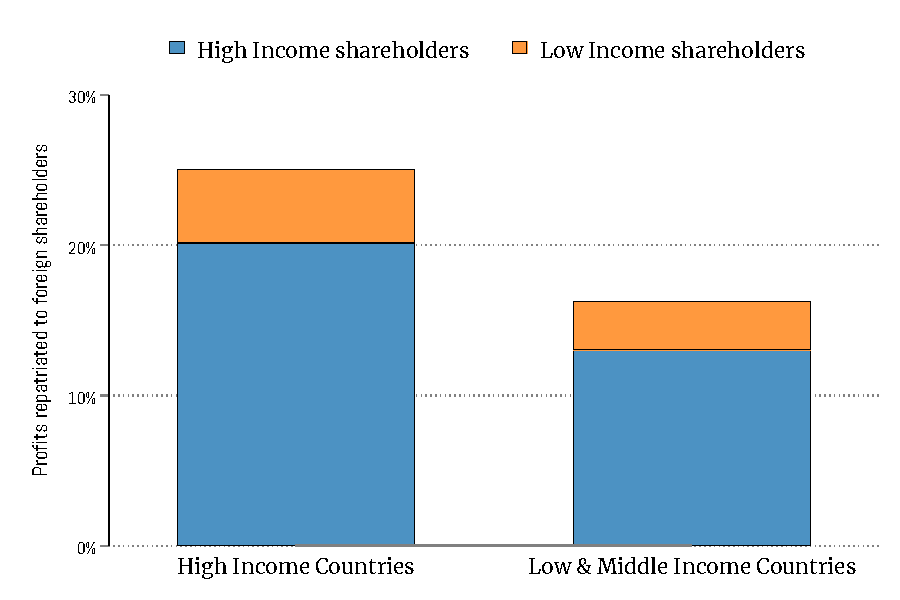
\includegraphics[scale=0.75]{Orbis/results/fig4}
\par\end{centering}
\vspace*{-7.5pt}%
\noindent\begin{minipage}[t]{1\columnwidth}%
\begin{spacing}{0.75}
{\footnotesize Note: The data is from Orbis. The share of profits repatriated
to foreign shareholders are inferred from equity shares in multinational
enterprises, using the algorithm described in Appendix \ref{sec:Data Appendix}.
The income group classification of countries is based on the \href{https://www.un.org/en/development/desa/policy/wesp/wesp_current/2014wesp_country_classification.pdf}{United Nations Country Classification}.}
\end{spacing}
%
\end{minipage}
\end{figure}


\subsection{Global Markup Estimation }

We estimate markups using two different approaches: The cost-based
approach and the demand-based approach. While both approaches are
well-understood, their macro-level implications have been rarely contrasted.
In part, because the demand-based approach has proven difficult to
implement at scale across a wide range of countries and industries.

\subsubsection{Demand-Based Markup Estimation.}

Markups can be recovered from demand elasticities, but demand estimation
at scale presents several challenges. First, we must impose parametric
assumptions to make progress. To navigate this issue without loss
of generality, we estimate a mixed multinomial logit model (MMNL)
which can approximate our semi-parametric demand system as closely
as possible.\footnote{This claim follows from \citet{thisse2016can}, who show that the
homothetic with an aggregator demand system can be alternatively derived
from a random utility model; and from \citet{mcfadden2000mixed} who
establish that any random utility model can be approximated as closely
as needed by the MMNL model.} Second, the conventional approach to estimating the MMNL model, introduced
by \citet[ BLP hereafter]{berry1995automobile}, is computationally
demanding, making it impractical to perform over thousands of product
categories. To tackle this issue, we employ a log-linear approximation
of the MMNL model proposed by \citet{salanie2019fast}, which is considerably
simpler to estimate. The final difficulty lies in the data requirements
for large-scale demand estimation. The standard BLP approach leverages
data on observable product characteristics to achieve identification,
but globally representative data on observed product characteristics
is unavailable. We overcome this obstacle by leveraging high-frequency
trade and exchange rate data to guide identification, eliminating
the need for data on product characteristics.

Before diving into our estimation strategy, let us provide a high-level
overview of the MMNL model, which forms the foundation of our estimation.
Consider a market populated by an infinite number of households, each
of which chooses one product variety from the set $\Omega_{kt}$ of
products available in industry $k$ in year $t$. There is also an
outside good, the indirect utility of which is normalized to 0. Assuming
that the idiosyncratic taste for product varieties is distributed
\emph{iid} according to a type-I Extreme Value distribution with scale
parameter 1, the market share of variety $\omega\in\Omega_{kt}$ can
be specified as
\[
\lambda_{\omega t}=\mathbb{E}_{\boldsymbol{\epsilon}}\left[\frac{\exp\left(\left(\overline{\boldsymbol{\beta}}_{kt}+\boldsymbol{\epsilon}\right)\cdot\textbf{X}_{\omega t}+\xi_{\omega t}\right)}{1+\sum_{\omega'\in\Omega_{i,kt}}\exp\left(\left(\overline{\boldsymbol{\beta}}_{kt}+\boldsymbol{\epsilon}\right)\cdot\textbf{X}_{\omega't}+\xi_{\omega't}\right)}\right],
\]
In this equation, $\textbf{X}$ represents a vector of \emph{observed}
product characteristics, such as prices, and $\overline{\boldsymbol{\beta}}$
denotes the mean coefficients on these characteristics. $\boldsymbol{\epsilon}$
is a random coefficient that follows an \emph{iid} distribution $N\left(0,\boldsymbol{\Sigma}_{kt}\right)$,
where $\boldsymbol{\Sigma}_{kt}$ is a diagonal variance matrix.\footnote{More specifically, the utility of household $h$ derives from purchasing
variety $\omega$ is $\left(\overline{\boldsymbol{\beta}}_{kt}+\boldsymbol{\epsilon}_{h,kt}\right)\cdot\textbf{X}_{\omega t}+\xi_{\omega t}+u_{\omega t}\left(h\right)$,
where $u$ accounts for idiosyncratic heterogeneity in taste for product
varieties, which is distributed \emph{iid} according to a type-I Extreme
Value distribution with scale parameter 1.} The demand shifter, $\xi$, captures \emph{unobserved} product characteristics,
such as perceived product quality at the market level. The BLP approach
to estimating demand recovers $\boldsymbol{\xi}$ by inverting the
market share equation and using the recovered values to enforce the
moment condition $\mathbb{E}\left[\Delta\boldsymbol{\xi}\mid\textbf{z}\right]=0$,
where $\textbf{z}$ represents a set of price instruments. The inversion
approach, however, is computationally challenging, particularly for
large-scale applications. To overcome these computational hurdles,
\citet{salanie2019fast} propose an alternative approach that approximates
$\boldsymbol{\xi}$ using the following equation:
\[
\xi_{\omega t}=\ln\left(\lambda_{\omega t}/\lambda_{0}\right)-\overline{\boldsymbol{\beta}}_{kt}\cdot\textbf{X}_{\omega t}-\tilde{\boldsymbol{\Sigma}}_{kt}\cdot\textbf{K}_{\omega t}+O\left(\parallel\boldsymbol{\Sigma}_{kt}\parallel^{2}\right),
\]
where $\tilde{\boldsymbol{\Sigma}}_{kt}=\text{Tr}\left[\boldsymbol{\Sigma}_{kt}\right]$
and $\textbf{K}$ is an \emph{artificial} regressor whose elements
are:
\[
K_{\omega t}\equiv X_{\omega t}\left[\,\frac{1}{2}\,X_{\omega t}\,-\mathbb{E}_{\lambda_{t}}[X]\right],\qquad with\qquad\mathbb{E}_{\lambda_{t}}[X]=\sideset{}{_{\Omega_{i,kt}}}\sum\lambda_{\omega t}X_{\omega t}
\]
 Following this approach and omitting higher-order terms, we obtain
an approximated value for $\xi$, denoted by $\check{\xi}$ . We then
estimate the demand parameters by exploiting the moment condition
$\mathbb{E}\left[\Delta\check{\xi}\mid\textbf{z}\right]=0$, which
is similar to running a linear 2SLS regression.\footnote{We instrument $\Delta K_{\omega t}$ using the number of alternative
product codes served by the firm in a year as an additional instrument.
See Appendix \ref{sec: Demand-Based-Markup-Estimation} for more details.} Given that $\ln p\subset\textbf{X}$, markups are recovered as $\mu_{\omega t}=\frac{\partial\ln\lambda_{\omega t}}{\partial\ln p_{\omega t}}(1+\frac{\partial\ln\lambda_{\omega t}}{\partial\ln p_{\omega t}})^{-1}$,
assuming single-product and profit-maximizing firms.

The next challenge is finding a valid instrument to guide identification
with limited data on observed product characteristics. Our dataset
reports three observable characteristics: the country of origin, the
product classification used by the statistical agency, and the unit
price ($p$). The demand residual \emph{conditional} on these characteristics,
$\tilde{\xi}$, is presumably contaminated with omitted variables
correlated with $p$---unlike small-scale estimations like BLP, where
$\xi$ is purged from a wider range of observable product characteristics
using richer data. To overcome this identification challenge, we leverage
high-frequency transaction data and interact it with high-frequency
exchange rate data to construct a granular shift-share instrument
for $\ln p$ that measures the exposure to exchange rate fluctuations
at the variety level and is uncorrelated with $\tilde{\xi}$. We begin
with the observation that the year-over-year change in the unit price
of variety $\omega$ can be approximated by the sales-weighted average
of monthly price changes: $\Delta\ln p_{\omega t}=\sum_{m\in\mathbb{M}_{t}}\lambda_{\omega t}\left(m\right)\Delta\ln p_{\omega t}\left(m\right)$,
where $\lambda_{\omega t}\left(m\right)$ and $p_{\omega t}\left(m\right)$
denote month $m$'s share of export sales and the year-over-year change
in export prices in month $m$ of year $t$ (i.e., $m\in\mathbb{M}_{t}$).
Since $p_{\omega t}\left(m\right)$ is denominated in the destination
market's currency, it varies with the year-over-year change in the
exchange rate between variety $\omega$'s origin country and the destination
market it serves in month $m$, denoted as $\mathscr{E}_{t}\left(m\right)$.
Motivated by this accounting relationship, we construct the shift-share
instrument: $z_{\omega t}=\sum_{m\in\mathbb{M}_{t}}\lambda_{\omega t-1}\left(m\right)\Delta\ln\mathscr{E}_{t}\left(m\right)$.
This instrument interacts the lagged export share $\lambda_{\omega t-1}\left(m\right)$
with the concurrent exchange rate change per month to measure variety-level
exposure to aggregate exchange rate fluctuations. The exposure measure
$z$ is uncorrelated with $\tilde{\xi}$ under the identifying assumption
that aggregate exchange rate fluctuations and past export composition
are independent of \emph{unobserved} concurrent demand shocks.

Our estimation uses the universe of import transactions for Colombia
from 2007 to 2016. The dataset encompasses over 93,000 firms from
251 different countries and reports high-frequency transaction-level
sales and quantities for individual firms exporting to Colombia at
the Harmonized System 10-digit product level. We complement this data
with matching high-frequency exchange rate data from the Bank of Canada
for the same time period. To fully leverage the granularity of our
data, we conduct our estimation using market share and price data
for 10-digit product categories. However, to ensure compatibility
between our estimated markups and the level of aggregation in the
ICIO data, we pool all 10-digit product categories and estimate demand
parameters at the ICIO industry level. Appendixes \ref{sec:Data Appendix}
and \ref{sec: Demand-Based-Markup-Estimation} provide further details
about our data and estimation methodology.

\subsubsection{Cost-Based Markup Estimation.}

Our cost-based approach to markup estimation closely follows \citet{de2012markups}.\footnote{We should note that the identifying assumptions underlying this approach
align more closely with our extended model, which explicitly incorporates
intermediate inputs (see Appendix \ref{sec: Appendix IO}). This extended
model is used for the quantification presented in the next section.} It builds on the observation that firm markups can be calculated
based on cost minimization as $\mu_{\omega}=\alpha_{\omega}p_{\omega}q_{\omega}/\mathcal{C}_{\omega}$
for $\omega\in\Omega_{kt}$, where $\mathcal{C}_{\omega}$ denotes
the variable inputs cost and $\alpha_{\omega}$ is the firm-level
output elasticity with respect to variable inputs. Since estimating
the output elasticity at the firm level is practically infeasible,
the standard approach to markup estimation recovers the output elasticity
under the simplifying restriction that all firms within product category
$k$ use the same production function. Under this restriction, we
can estimate the industry-wide output elasticity ($\alpha_{\omega}\coloneqq\alpha_{kt}$
for all $\omega\in\Omega_{kt}$) using the control function approach
in \citet{olley1996dynamics}.\footnote{In the first stage, we purge output of measurement error and unanticipated
shocks by regressing it on a second-order polynomial of inputs and
investment. In the second stage, we estimate the output elasticities
by fitting an AR(1) process for productivity and leveraging moment
conditions that impose orthogonality between implied productivity
and lagged variable inputs and current capital inputs. The estimation
uses firm-level financial accounts data from \noun{Compustat} North
America. The data is reported based on the SIC industry classification.
So, we concord SIC industries into the 36 ICIO industries to mach
our macro-level trade and production data. For each industry and year
during the 2005-2015 period, we separately estimate the output elasticity
using the control function method. Since panel data are required for
the control function estimation, we employ 5-year rolling windows,
assigning the elasticity estimates derived from data in years $t-2$
to $t+2$ the central year $t$.} Since balance sheet data record expenditure and sales rather than
physical quantities, the structural error term in the production function
is contaminated with unobserved prices shifter such as markups. Following
\citet{de2020rise}, we control for unobserved markups using firms'
sales shares within industries.

We then compute firm-level markups using internationally-representative
data from the \noun{Worldscope} \noun{Global} \noun{Database}. The
data reports the cost of variable inputs $\mathcal{C}_{\omega}$ and
sales $p_{\omega}q_{\omega}$ across 71,546 publicly traded firms
from 134 countries during the 2005 -2015 period. Some firms in this
database operate in more than one industry, but we do not observe
the breakdown of firm-level sales and costs by industry. To handle
this, we assume that sales and costs are equally spread across different
products. Following \citet{de2018global}, we assume that the output
elasticity is the same across countries. Letting $\hat{\alpha}_{kt}$
denote the estimated output elasticity in industry $k$, we calculate
the markup charged for variety $\omega\in\Omega_{kt}$ as $\mu_{\omega}=\hat{\alpha}_{kt}p_{\omega}q_{\omega}/\mathcal{C}_{\omega}$.
We then compute the harmonic sales-weighted average markup in industry
$k$ as $\widetilde{\mathbb{E}}_{\lambda}\left[\mu\right]=\left[\sum_{\omega\in\Omega_{kt}}\lambda_{\omega}\mu_{\omega}^{-1}\right]^{-1}$,
where $\lambda_{\omega}$ is firm $\omega$'s sales share within $\Omega_{kt}$.
Figure \ref{fig: markup} in the appendix reports $\widetilde{\mathbb{E}}_{\lambda}\left[\mu\right]$
derived from our cost-based markup estimates across various ICIO industries.

\paragraph*{Estimation results.}

Figure \ref{fig: Markup (B)} displays the estimated markups for
select manufacturing industries during 2005-2015, based on both demand-based
and cost-based approaches. The graph displays the arithmetic sales-weighted
average markup for each industry in a given year. Since our transaction-level
import data begins in 2007, our demand-based markup estimates (which
are obtained from a first-difference estimator) cover years after
2008. As anticipated, there are some discrepancies between the demand-based
and cost-based markup values. However, in many industries, the demand-
and cost-based markup estimates closely track each other over time.
As we show next, both markup estimates yield starkly similar macro-level
predictions about the loss from market power and the role of trade
specifically.

\begin{figure}[!tbh]
\caption{\label{fig: Markup (B)}The variation in estimated markups over time:
\emph{manufacturing industries}}

\begin{centering}
\hspace*{-15bp}\includegraphics{\string"ICIO data/Markup_Graph/fig3\string".pdf}
\par\end{centering}
\centering{}\vspace*{-0.15in}
\noindent\begin{minipage}[t]{1\columnwidth}%
\begin{spacing}{0.8}
{\footnotesize\emph{Note}}{\footnotesize : Cost-Based markups are estimated
using the }{\footnotesize\noun{Worldscope}}{\footnotesize{} and }{\footnotesize\noun{Compustat}}{\footnotesize{}
data. Demand-based markups are estimated using Colombian import transactions
from }{\footnotesize\noun{Datamyne}}{\footnotesize{} (see Appendix \ref{sec:Data Appendix}).
Industry classifications are based on the }{\footnotesize\noun{Icio}}{\footnotesize{}
}{\footnotesize\noun{Tables}}{\footnotesize .}
\end{spacing}
%
\end{minipage}
\end{figure}


\paragraph*{Model validation using estimated markups:}

A common implication of models featuring Pareto-distributed productivity
and separable demand, such as ours, is that, although countries may
differ in their aggregate markup distributions, they share a common
markup distribution \emph{within} narrowly defined industries. For
this prediction to hold empirically, the industry classification must
be sufficiently disaggregated. Using the ICIO industry codes, we assess
this requirement by examining whether within-industry markup distributions
are similar across countries. We do so by partitioning the \noun{Worldscope}
dataset into firms headquartered in high-income and low-/middle-income
economies. We then compare average markups at the industry level across
these two groups (Appendix Figure \ref{fig: markup-compariso}). The
results indicate that \emph{within-industry} average markups are virtually
identical across income groups, supporting the consistency of our
semi-parametric framework with the data. In short, the ICIO industry
classification is granular enough for our framework to be empirically
valid.

\subsection{The Welfare Loss from Market Power: A Global Perspective}

In this section, we report the aggregate loss from market power for
various countries, which is the sum of the welfare loss due to markup
dispersion and the country's exposure to international profit-shifting
externalities. We compute the welfare loss by plugging our estimated
markup values and share data into our semi-parametric formula for
$\mathscr{D}_{i}$. Figure \ref{fig: map main} presents the results
when multi-national profit payments are accounted for. The welfare
loss from market power is noticeably higher in low-income regions.
Remarkably, some high-income countries, such as the Netherlands, actually
benefit from markup distortions.\footnote{It is important to emphasize that without trade, all countries would
have experienced losses from markup distortions.} This indicates that for these countries, the positive gains from
profit-shifting more than offset the loss from markup dispersion.
However, as noted earlier, profit-shifting effects are zero-sum, meaning
that these benefits come at the expense of other nations, primarily
low-income ones.

\begin{figure}[!tbh]
\caption{\label{fig: map main} The welfare loss from market power across different
countries}

\begin{centering}
\includegraphics[scale=0.65]{\string"ICIO data/Appendix_Figures_Tables/Figure_12/figure_worldmap_main\string".png}
\par\end{centering}
\noindent\begin{minipage}[t]{1\columnwidth}%
\begin{spacing}{0.75}
{\footnotesize\emph{Note}}{\footnotesize : This map reports the aggregate
welfare loss from market power, measured as the per-cent loss in real
consumption due to monopolistic markups. The loss is calculated using
demand-based markup estimates in 2015 and accounts for multi-national
ownership. Data on industry-level expenditure and production are from
the }{\footnotesize\noun{Icio}}{\footnotesize . Data on multinational
ownership are from }{\footnotesize\noun{Orbis}}{\footnotesize .}
\end{spacing}
%
\end{minipage}
\end{figure}

We next examine whether the welfare loss from market power has increased
over time. Figure \ref{fig: F1} presents the findings, tracing the
change in the welfare loss from market power between 2005 and 2015.
The y-axis denotes the welfare loss, quantified as the percentage
loss in real consumption due to markup distortions. The figure presents
GDP-weighted averages for high-income and low/middle-income groups,
categorized according to the classification outlined in Table \ref{tab:List-of-countries}.
The left panel showcases the welfare loss calculated using demand-based
markup estimates, while the right panel displays results derived from
cost-based markup estimates. The results in Figure \ref{fig: F1}
point to substantial welfare losses, but it is important to recognize
that these estimates may still understate the true extent of the loss,
as they do not take into account the amplification from input-output
linkages demonstrated in Figure \ref{fig: F1 (IO linkages)} in the
appendix.\footnote{A higher substitution elasticity between aggregate industries also
amplifies the welfare loss from markup distortions. Figure \ref{fig: Fig8}
in the appendix shows that the welfare rises significantly with a
higher cross-industry elasticity of substitution. For the US, increasing
elasticity from 1 to 2 more than doubles the welfare loss from markups.
This is because resource allocation across industries becomes more
sensitive to markup distortions as substitutability increases.}

\begin{figure}[!tbh]
\caption{\label{fig: F1} The longitudinal change in welfare loss from market
power}

\vspace*{0.1in}
\begin{centering}
\includegraphics{\string"ICIO data/Decomposition/Fig_2\string".pdf}
\par\end{centering}
\noindent\begin{minipage}[t]{1\columnwidth}%
\begin{spacing}{0.75}
{\footnotesize\emph{Note}}{\footnotesize :}{\footnotesize\emph{ }}{\footnotesize The
above graph reports the aggregate welfare loss fro, markups and its
change over time for high versus low/middle income countries. A 5\%
loss implies that markups lower real national consumption by 5\% relative
to its efficient level. The welfare loss is calculated by plugging
our estimated markup values and output/expenditure share data into
our formula for $\mathscr{D}_{i}$, accounting for multinational profit
payments. The figures in the middle panel are computed by assuming
that output/expenditure shares and cross-country profit payments remain
constant at their 2005 level. The figures in the bottom panel are
computed by assuming that markups remain constant at their 2005 level.
Data on industry-level expenditure, trade, production shares are from
the }{\footnotesize\noun{Icio}}{\footnotesize .}
\end{spacing}
%
\end{minipage}
\end{figure}

Figure \ref{fig: F1} clearly illustrates that markups result in a
greater welfare loss for low-income countries compared to high-income
nations. Moreover, the welfare loss has been steadily increasing
over time, with the trend being particularly acute among low-income
nations. While these results are consistent with the existing literature
on the \emph{rise of market power}, there are two noteworthy aspects
that set our analysis apart. First, rather than focusing on the sales-weighted
average markup as \citet{de2020rise}, we directly quantify the welfare
loss of markups based on theoretical foundation. This distinction
is crucial, as the average markup can, in principle, increase without
necessarily leading to a greater welfare loss for the economy. Second,
prior studies have primarily relied on cost-based markup estimates
to document the rise in market power. However, Figure \ref{fig: F1}
suggests that the same pattern emerges even when demand-based markup
estimates are employed.

The lower panels in Figure \ref{fig: F1} decompose the change in
markup distortions into changes driven by $(1)$ adjustments to output
composition and multinational profit payment over time, and $(2)$
adjustments to markup levels over time. The middle panel takes a ceteris
paribus approach, holding output and expenditure shares constant at
their 2005 levels. This allows us to isolate the effect of changing
markup levels on the welfare loss measure, $\mathscr{D}_{i}$. Conversely,
the bottom panel keeps markups fixed at their 2005 levels and tracks
the change in $\mathscr{D}_{i}$ that can be attributed to shifts
in the economic composition. The results from these lower panels are
quite revealing. They demonstrate that the global increase in the
welfare loss from markups is entirely driven by changes in markup
levels over time. Meanwhile, the change in output composition and
multinational profit payment has merely redistributed the burden of
markup distortions, shifting it from high-income countries to their
low-income counterparts. These findings provide an initial glimpse
into the zero-sum nature of profit-shifting effects, which are formally
quantified in the following section.

\subsection{Profit-Shifting Effects: North-South Redistribution}

We invoke Proposition 2 to isolate how trade integration has shifted
the burden of markup distortions internationally. For completeness,
we measure the impact of trade under various considerations such as
multi-national ownership, global input-output linkages, and fixed
overhead costs that trim profits. It is important to note that from
the lens of our semi-parametric model, trade modifies the burden of
markup distortions primarily through profit-shifting effects. The
logic is that trade integration prompts specialization based on comparative
advantage, dampening the welfare loss from markups for countries that
specialize in high-markup product categories, while amplifying it
for others through profit-shifting.

Figure \ref{fig: F2} displays the change in the welfare loss from
markups due to trade integration, reporting average effects across
low- and high-income country groups. The results reveal that through
international profit-shifting, trade has shifted the burden of markups
from high-income nations to low-income countries. This finding is
also robust to the method used for markup estimation and persists
even after accounting for multi-national ownership, global input-output
networks, and fixed overhead costs. 

\begin{figure}[!tbh]
\caption{\label{fig: F2} The change in the welfare loss from market power
due to profit-shifting effects}

\vspace{0.1in}
\begin{centering}
\includegraphics{\string"ICIO data/Fig_2\string".pdf}
\par\end{centering}
\noindent\begin{minipage}[t]{1\columnwidth}%
\begin{spacing}{0.75}
{\footnotesize\emph{Note}}{\footnotesize : The above graph reports
the percent trade-induced change in the aggregate welfare loss from
market power. For example, a 5\% change represents to a 5\% increase
in the welfare loss from markups defined in Section \ref{sec: Cost of Markups}.
To top row reported results obtained from our baseline model using
Proposition 2. The next row accounts for multi-national ownership
(Equation \ref{eq: delat_D (MN ownership)}). the third account for
global input-output linkages as explained in Appendix \ref{sec: Appendix IO}.
The last row accounts for fixed overhead costs that trim profits as
detailed in Appendix \ref{sec:Proof P4}. Data on industry-level expenditure,
production and input-output shares are from the }{\footnotesize\noun{Icio}}{\footnotesize .
Data on global profit ownership are from }{\footnotesize\noun{Orbis}}{\footnotesize .
Cost-Based markups are estimated using data from }{\footnotesize\noun{World
Scope}}{\footnotesize{} and demand-based markups are estimated using
transaction level import data from Colombia provided by }{\footnotesize\noun{Datamyne}}{\footnotesize .}
\end{spacing}
%
\end{minipage}
\end{figure}

Our findings, averaged across all years and specifications (such as
demand-based and cost-based markup estimation), indicate that trade
integration has had a significant impact on the welfare loss from
markups for low- and middle-income countries. On average, it has increased
the welfare loss for these countries by 44\% while simultaneously
reducing it by 15\% among high-income nations. These effects represent
substantial transfers between countries that occur primarily through
international profit-shifting, a phenomenon that has been largely
overlooked in previous literature. The existing literature has mainly
focused on the pro-competitive effects of trade, which reduce markup
dispersion and are internationally symmetric, with some studies finding
these effects to be relatively small.

The asymmetric effects of trade on the loss from market power become
even more pronounced when considering the role of multi-national ownership
and the repatriation of profits to foreign shareholders. This finding
is consistent with our previous empirical observation that profits
earned by multi-national corporations are primarily repatriated to
shareholders in high-income countries. When global input-output (IO)
linkages are accounted for, the impact of trade is somewhat attenuated,
although the directionality of the effects remains the same. This
attenuation occurs because IO linkages amplify the welfare loss of
markup dispersion while diluting the extent of profit-shifting, making
the profit-shifting component of the welfare loss less consequential.
When fixed overhead costs are considered, the asymmetric effects of
trade are amplified, suggesting that fixed cost payments incurred
in foreign markets contribute to profit-shifting, as low-income countries
paying net quasi-rents to high-income partners in the form of fixed
cost payments.

It is important to note that the results emerging from Figure \ref{fig: F2}
are not apparent a priori. While profit-shifting effects are zero-sum
by nature, there is no inherent reason to believe that they favor
high-income countries. That being said, Figure \ref{fig: F2} masks
the heterogeneity in exposure to profit-shifting within income groups.
To delve deeper into this aspect, Figures \ref{fig: map appendix (a)}
and \ref{fig: map appendix (b)} in the appendix provide a more granular
visualization of the impacts of profit-shifting effects, highlighting
heterogeneous effects even within low and middle-income groups. For
example, profit-shifting is less detrimental for the Chinese economy
but extremely costly for African countries.\footnote{For most countries, the impacts of international profit-shifting have
a stable sign across specifications. In a few instances, however,
accounting for input-output linkages or firm-selection reverses our
baseline predictions. } Relatedly, Figure \ref{fig: Fig6} in the appendix visualizes the
flow of  excess profits on a bilateral basis, although interpreting
these flows is more intricate due to issues related to balanced trade
and the fact that these flows do not directly translate to welfare
effects without proper normalization.

\subsection{A New Perspective on Tariff Reciprocity}

Section \ref{sec: Implications-for-Policy} demonstrated that, under
certain conditions, firm markups act as de facto shadow tariffs. The
resulting profit-shifting externalities from decentralized markups
mirror the terms-of-trade effects typically associated with asymmetric
tariffs. This equivalence has important implications for tariff reciprocity
under current trade agreements. This section empirically tests the
equivalence by identifying a shadow tariff schedule that replicates
the distributive effects of decentralized markups. The quantitative
methodology is outlined in Appendix \ref{sec: Hat-Algebra Tariff}
which derives a shadow tariff schedule, $\{\check{t}_{i}\}$, that
reproduces the aggregate welfare impact of firm markups. The resulting
effective tariff is defined as $t_{i}+\check{t}_{i}$, where $t_{i}$
denotes the applied (or explicit) tariff.

Figure \ref{fig: F3} compares effective tariffs with applied tariffs.
At first glance, high-income countries appear to levy lower tariffs
than low-income countries, consistent with the WTO\textquoteright s
Generalized System of Preferences (GSP). In 2015, high-income countries
had a weighted average applied tariff of just 2.3\%, compared to 5.9\%
for low- and middle-income countries---suggesting greater tariff
concessions by wealthier economies under the WTO framework. However,
once shadow tariffs from markup distortions are incorporated, the
effective tariff landscape shifts considerably. For high-income countries,
the effective tariff rises to 19.9\%. Thus, contrary to the intended
spirit of the GSP, high-income countries effectively impose an excess
tariff of 14\% (= 19.9\% -- 5.9\%) on imports from low-income trading
partners. 

\begin{figure}[!tbh]
\caption{\label{fig: F3}Tariff Reciprocity: applied tariffs vs effective tariffs }
\*\vspace{0.1in}
\begin{centering}
\includegraphics[scale=1.25]{\string"ICIO data/Figure_3\string".pdf}\*\vspace{-0.1in}
\par\end{centering}
\noindent\begin{minipage}[t]{1\columnwidth}%
\begin{spacing}{0.8}
{\footnotesize Note: This figure reports the effective tariffs (applied
tariffs + implicit tariffs due to profit-shifting effects) and compares
them to applied tariffs for each country group. The tariff rates for
each country group are the GDP-weight average rates and calculated
using the algorithm described in Appendix \ref{sec: Hat-Algebra Tariff}.
To handle the one degree pf freedom redundancy in nominal variables,
the average effective tariff rate among low-income nations is normalized
to the average applied rate. Our calculation uses expenditure and
output data from the}{\footnotesize\textsc{ ICIO}}{\footnotesize{} tables
and our estimated markups (described in Section \eqref{sec: Quantitative })
in year 2015. Industry-level trade elasticity values are from \citet{caliendo2015estimates}.}
\end{spacing}
%
\end{minipage}
\end{figure}

These results state that the monopolistic objective of firms in high-income
countries aligns with the government's desire to manipulate the terms
of trade---possibly, discouraging regulation of anti-competitive
behaviors that would otherwise be addressed in a closed economy. Accordingly,
while monopolistic pricing practices reflect a domestic policy failure
in a closed economy, they amount to a negative international externality
in a global setting. Shallow cooperation, thus, entails that governments
tackle the profit-shifting externality to prevent adverse impacts
on their trading partners, at least based on the basic principles
underlying the WTO.

The first-best policy to address profit-shifting externalities is
internationally coordinated markup correction. However, implementing
this solution is challenging within the WTO's current framework, which
focuses on regulating and coordinating border policies rather than
domestic policy measures. Therefore, we explore two alternative policy
solutions in Appendix \ref{sec:Policy-Remedies}. The first leverages
existing mechanisms within the WTO, advocating for a revised interpretation
of the reciprocity principle. The second solution could be integrated
into the evolving global minimum tax agreement.

\subsection{Discussion: Mechanism and Limitations}

This section provides some explanations for the pro-rich bias of profit-shifting
effects and examines why these effects have diminished over time.
We also discuss limitations that should be taken into account when
interpreting our findings\emph{.\medskip{}
}\\
\emph{Mechanism.$\quad$}Based on our formulas, countries that specialize
in high-markup industries benefit from profit-shifting at others'
expense. Figure \ref{fig: F2} indicates that high-income countries
are the primary beneficiaries, raising the question of what drives
this pattern. Theory offers several explanations: \citet{fajgelbaum2011income}
and \citet{lashkaripour2020within} argue that high-income countries
have a natural comparative advantage in high-markup industries. In
the former, comparative advantage is driven by the home-market effect.
In the latter, it is driven by higher input costs in rich countries,
which favor production of less price-elastic, high-markup goods. Another
explanation is based on differences in factor endowments and institutional
quality across countries. Appendix \ref{sec: Appendix Origins} shows
that better legal and credit-market institutions are associated with
specialization in high-markup industries, leading to net gains from
profit-shifting. By contrast, natural-resource abundance correlates
with losses, consistent with the resource curse. Overall, institutions
that promote specialization in high-markup industries are generally
correlated with income, thereby explaining the pro-rich bias of international
profit-shifting.\emph{\medskip{}
}\\
\emph{Longitudinal Trends.$\quad$}Figure \ref{fig: F2} indicates
that profit-shifting from low- to high-income nations may have dampened
over time. This trend can be attributed to two possible factors. First,
middle-income nations may have become more specialized in high-markup
industries between 2005 and 2015. Second, markup levels may have evolved
in a way that dampens profit-shifting from low-to-high-income nations.
We examine these two possibilities in Appendix \ref{sec: Appendix Evolution}.
Our analysis reveals that the dampening effect is almost entirely
explained by changes in North-South specialization patterns. That
is, low and middle income nations have become increasingly specialized
in sophisticated, high-markup industries, dampening the extent to
which profits flow out of these economies to high-income trading partners---demonstrated
by the bottom panel of Figure \ref{fig: Evolution Rent-Shifting}
in Appendix \ref{sec: Appendix Evolution}.\footnote{We use a static classification of countries from the United Nations
when dividing our sample into low- and high-income countries. An alternative
approach is to classify countries according to their real GDP per
capita. The reduced-form analysis conducted using this alternative
classification in Appendix \ref{sec:Motivating-Evidence} does not
suggest a dampening of North-South profit-shifting effects.}\emph{\medskip{}
}\\
\emph{Limitations.$\quad$}Several limitations are worth noting. Our
markup estimation is subject to the usual limitations. Our cost-based
markup estimates draw from publicly listed firms\textquoteright{}
balance sheets, and may not be fully representative.  The demand-based
approach recovers the markup distribution based on what global firms
charge in the Colombian market. Under our theoretical framework, the
recovered distribution for each product can be extrapolated to other
markets.\footnote{Specifically, while individual firms do pursue pricing-to-market in
our framework, the aggregate markup distribution remains the same
across markets due to firm-selection effects.} So, to the extent that our Pareto and demand assumptions hold, the
demand-based markups are globally representative. Here, the close
alignment between demand- and cost-based markups is reassuring. A
second limitation is that we measure only output market power. This
poses two issues. First, markups derived from revenue elasticities
may reflect not output-side markups but input-side markdowns arising
from monopsony power (\citet{bond2021some}).\footnote{Two points are worth highlighting in relation to this concern: (a)
our demand-based markup estimates are immune to this critique; and
(b) \citet{de2022hitchhiker} find that although revenue-based data
may bias markup levels, the correlation between the estimated and
actual markup remains strong.} Second, if markdowns---not markups---drive the wedge, trade would
intensify monopsony distortions for workers in countries facing larger
markdowns, likely those in high-income economies.

\section{Conclusion}

\begin{singlespace}
The global rise in market power and trade openness are two hallmarks
of the current economic era. We show that these developments have
led to substantial welfare transfers from low-income to high-income
countries through international profit-shifting externalities. These
effects are akin to implicit tariffs that distort the terms of trade
in favor of high-income countries. This observation suggests that,
contrary to prevailing wisdom, low-income countries have made greater
concessions under the current system of global trade agreements. To
create a more level playing field, we propose two policy reforms that
can mitigate the burden of international profit-shifting on low-income
countries. The first reform involves high-income countries making
unilateral tariff concessions under the WTO's Generalized System of
Preferences (GSP) mechanism. The second reform entails the implementation
of a destination tax on profits, which, while only partially effective,
may be more viable from a political economy standpoint. These policy
solutions require international coordination among cooperative governments.
In the absence of such cooperation, countries must resort to second-best
unilateral policy remedies. Characterizing the optimal design of unilateral
policy remedies and evaluating their effectiveness presents a promising
avenue for future research.\singlespacing
\fontsize{10.5}{12}\selectfont 

\bibliographystyle{chicago}
\bibliography{DLL2021}


\appendix
\onehalfspacing
\newgeometry{left=1in, right=1in, top=1in, bottom=1in, footskip=0.65cm}
\fontsize{11.5}{12}\selectfont 
\setcounter{table}{0} 
\renewcommand{\thetable}{A.\arabic{table}} 
\setcounter{atable}{0}
\setcounter{figure}{0}
\renewcommand{\thefigure}{A.\arabic{figure}} 
\setcounter{afigure}{0}
\numberwithin{equation}{section}
\pagenumbering{arabic}
\setcounter{assumption}{0}
\end{singlespace}

\part*{Data Appendix{\Large{} (for online publication)}}

\section{\label{sec:Data Appendix}Data Sources}

\subsection{\noun{Unido-Indstat}}

This dataset is provided by the \noun{United Nations Industrial Development
Organization} (UNIDO), and is accessible through the UNIDO Data Portal.
The data can be downloaded after registering for access on the UNIDO
website, and it includes comprehensive industrial statistics covering
a wide range of countries, years, and industries. We use the subsample
corresponding to the 1980-2015 period, covering 196 countries and
23 ISIC rev.3 industries. For each industry and country in a given
year, the data reports output, value added, wages and salary payments,
number of employees, number of establishments, and gross fixed capital
formation, among other variables. We use these variables to calculated
aggregate accounting profits margin for each \emph{industry-country-year}
triad. We supplement this data with its derivative, the \noun{TradeProd
}database, developed and maintained by the \noun{Cepii}. Users can
access the TradeProd database through the official CEPII web portal
after registration, which requires basic information and agreement
to the terms of use. The \noun{TradeProd }database only covers manufacturing
industries, which are more traded and spans fewer years than the \noun{Unido-Indstat}
data. However, it reports domestic absorption measures per industry,
allowing us to calculate net exports for each \emph{industry-country-year}
triad.

\subsection{\noun{The OECD Inter-Country Input-Output (ICIO) Tables.\label{subsec:The-OECD-Inter-Country}}}

The ICIO Tables (2018 edition) provides comprehensive information
on international trade and production across major global economies.
This dataset includes a sample of 64 major countries, covering 36
industries that span the entire economy from 2005 to 2015.\footnote{ICIO tables include 64 countries (i.e. 36 OECD countries and 28 non-OECD
economies), the Rest of the World and split tables for China and Mexico.
In our analysis, we exclude the split tables for China and Mexico
(i.e. CN1, CN2, MX1, and MX2).} The dataset reports extensive information on trade flows across various
origin-destination pairs and national level input-output tables disaggregated
at the ICIO sector level. Users can access the ICIO data through the
official \href{https://www.oecd.org/sti/ind/inter-country-input-output-tables.htm}{OECD web portal}
after registration which requires basic user information and agreement
to the terms of use. We use the ICIO data to construct country and
industry-level output and expenditure shares ($y_{i,k}$ and $e_{i,k}$)
as well as national-level input-output shares, $\alpha_{i,gk}$. In
particular, from the ICIO tables, we can observe $X_{ni,k}$, which
is the total flows of industry $k$ goods from origin country $n$
to destination country \emph{$i$.} The expenditure share $e_{i,k}$
and output shares $y_{i,k}$ of country $i$ in industry $k$ in the
baseline model are constructed as follows with this information:
\[
e_{i,k}=\frac{\stackrel[n=1]{65}{\sum}\left(X_{ni,k}\right)}{\stackrel[g=1]{36}{\sum}\stackrel[n=1]{65}{\sum}\left(X_{ni,g}\right)},\qquad\qquad\qquad y_{i,k}=\frac{\stackrel[n=1]{65}{\sum}\left(X_{in,k}\right)}{\stackrel[g=1]{36}{\sum}\stackrel[j=1]{65}{\sum}\left(X_{in,g}\right)}
\]


\subsection{\noun{Compustat -- North America}}

We conduct the production function estimation per industry using firm-level
financial accounts data from \noun{Compustat} \noun{-- North America},
which provides rich coverage regarding capital inputs and firm-level
investments for publicly held companies in the United States and Canada.
This database provided by \noun{S\&P Global Market Intelligence} and
can be accessed through the \noun{Wharton Research Data Services}
(WRDS) platform, which requires an institutional subscription. Users
affiliated with subscribing institutions can download the data after
logging into the WRDS platform and navigating to the \noun{Compustat
-- North America} database. The data is reported based on the SIC
industry classification. So, we concord SIC industries into the 36
ICIO industries for which we have macro-level trade and production
data using the following steps:
\begin{description}
\item [{(a)}] we obtain the full sample of companies during the period
2003-2017 from the \noun{Compustat} \noun{-- North America} database. 
\item [{(b)}] we deflate firms' sales, cost of good sold, capital expense,
staff expense, and general administrative expanse by U.S. GDP.
\item [{(c)}] we drop observations with negative sales, cost of good sold,
capital expense, staff expense, general administrative expanse, and
sales-to-cost ratio. 
\item [{(d)}] since the database only reported the SIC industry classification,
we have to concord SIC industries into the 36 ICIO industries for
which we have macro-level trade and production data discussed in Section
\ref{subsec:The-OECD-Inter-Country}. Unfortunately, we do not have
official correspondence table mapping SIC to ICIO industry classification.
Therefore, we concord SIC to ICIO by the following steps:
\[
SIC\overset{(a)}{\rightarrow}ISIC\:rev.3\overset{(b)}{\rightarrow}ISIC\:rev.3.1\overset{(c)}{\rightarrow}ISIC\:rev.4\overset{(d)}{\rightarrow}ICIO
\]
\end{description}
The official correspondence tables of steps (a)-(c) can be found on
the website of \href{https://unstats.un.org/unsd/classifications/Econ/isic}{United Nation};
and the correspondence table of step (d) can be found on the data
descriptions from OECD Inter-Country Input-Output (ICIO) Tables. In
addition, we also check and correct the correspondence tables manually
by the verbal descriptions of each industry classifications to make
sure we have the best match from SIC to ICIO. This step gives us 21,386
firms operating across 36 ICIO industries in United States and Canada
from 2003 to 2017. After complaining the final data, we separately
estimate the output elasticity for each industry and year during the
2005-2015 period using the control function method described in the
main text.

\subsection{\noun{Worldscope}}

\noun{Worldscope} is a database provided by \noun{Thomson Reuters},
containing financial statement data and other financial information
for publicly traded companies worldwide. The database can be accessed
through the \noun{Thomson Reuters Eikon} platform or \noun{Datastream},
both of which require a subscription. Users with access to these platforms
can download the data by searching for the desired firms and variables
within the \noun{Worldscope} database. In this paper, we process the
data by the following steps:
\begin{description}
\item [{(a)}] we download firm-level data of sales and costs of good sold
from the \noun{Worldscope} database during the 2005 - 2015 period.
\item [{(b)}] we drop observations with negative values on sales or costs
of good sold. This steps give us 71,546 publicly traded firms operating
across 987 SIC industries in 134 countries.
\item [{(c)}] some firms in this database operate in more than one industry,
but we do not observe the breakdown of firm-level sales ($y$) and
input costs ($c$) by industry. We treat a particular firm that operates
in $n$ SIC-industries as $n$ different single product firms, and
each firm is assumed to have sales as $y/n$ and cost as $c/n$. Then
we can calculate firm's cost-sales ratio that will be used in the
cost-based markup estimation process. 
\end{description}
Table \ref{tab:Summary-Statistics-for-Worldscope} reports the summary
statistics including the average number of unique firms per country,
the average number of industries served per firm, the average sales
per firm, and the average input cost per firm . We report statistics
for 63 main countries/regions in the ICIO database and the rest of
the world.

\begin{table}[!tbph]
\vspace*{-25pt}
\caption{\noun{\label{tab:Summary-Statistics-for-Worldscope}Worldscope} database:
Summary Statistics}

\vspace*{-1bp}

\begin{raggedright}
\vspace{-0.3in}
\begin{center}  
	\adjustbox{max height=0.5\textheight}{\begin{tabular}{lcccc}  
			\toprule 
			
			{Country}&&{avg number of industries }&{sales per firm}&{input cost per firm} \\
			& {number of firms} &{operated per firm}&{(local currency)}&{(local currency)} \\
			\midrule \addlinespace[\belowrulesep]
			Argentina&107&4&3,253.1&1,813.2 \\
			Australia&2,041&3&462.9&259.7 \\
			Austria&102&4&1,446.5&823.8 \\
			Belgium&158&3&1,667.7&656.9 \\
			Brazil&429&4&4,750.4&2,392.2 \\
			Bulgaria&263&4&49.0&25.6 \\
			Cambodia&2&2&489,229.6&202,954.6 \\
			Canada&3,404&2&423.4&239.0 \\
			Chile&259&4&441,967.3&303,846.5 \\
			China&3,276&4&6,680.0&4,165.4 \\
			Colombia&79&5&2,139,877.0&1,089,354.0 \\
			Costa Rica&8&5&96,564.8&69,893.0 \\
			Croatia&114&5&1,127.9&798.9 \\
			Cyprus&128&3&75.4&43.3 \\
			Czechia&22&4&23,636.5&13,260.9 \\
			Denmark&373&3&3,571.3&3,264.2 \\
			Estonia&17&5&145.3&106.9 \\
			Finland&149&4&1,232.5&897.4 \\
			France&900&3&2,456.7&1,439.0 \\
			Germany&970&3&2,522.1&1,546.9 \\
			Greece&300&4&346.9&192.4 \\
			Hong Kong (China)&1,337&5&6,034.8&3,392.7 \\
			Hungary&47&3&164,571.6&108,459.8 \\
			Iceland&20&4&46,048.8&31,444.5 \\
			India&2,757&3&16,401.4&11,923.3 \\
			Indonesia&494&3&3,392,747.0&2,217,032.0 \\
			Ireland&79&3&1,286.8&832.1 \\
			Israel&546&3&1,330.9&785.4 \\
			Italy&336&4&2,605.7&1,213.4 \\
			Japan&4,064&5&177,394.3&122,260.1 \\
			Kazakhstan&62&3&72,720.4&37,474.9 \\
			Korea&1,870&4&1,050,410.0&758,646.7 \\
			Latvia&32&3&46.7&34.3 \\
			Lithuania&37&4&106.9&76.2 \\
			Luxembourg&65&3&2,156.2&1,860.3 \\
			Malaysia&1,059&5&959.4&611.1 \\
			Malta&22&3&57.0&13.1 \\
			Mexico&160&5&36,555.2&24,466.9 \\
			Morocco&76&3&3,248.9&2,145.1 \\
			Netherlands&208&4&4,730.3&3,059.1 \\
			New Zealand&176&3&510.5&342.4 \\
			Norway&270&3&6,537.8&3,950.7 \\
			Peru&182&4&877.8&481.2 \\
			Philippines&269&3&14,483.7&10,044.4 \\
			Poland&531&4&965.8&661.6 \\
			Portugal&59&5&1,426.4&1,035.8 \\
			Rest of World&2,822&3&13,700,000.0&728,454.4 \\
			Romania&162&4&406.3&240.1 \\
			Russian&992&3&34,532.2&16,526.5 \\
			Saudi Arabia&153&5&3,252.6&2,208.9 \\
			Singapore&714&4&587.1&418.0 \\
			Slovakia&25&4&298.1&248.2 \\
			Slovenia&54&5&275.5&206.4 \\
			South Africa&388&4&8,433.9&4,943.3 \\
			Spain&192&5&3,030.8&1,650.8 \\
			Sweden&602&3&5,804.3&3,539.6 \\
			Switzerland&302&4&3,126.6&1,294.5 \\
			Chinese Taipei &1,839&3&14,360.8&11,022.7 \\
			Thailand&666&4&13,478.8&10,678.3 \\
			Tunisia&65&3&154.9&90.5 \\
			Turkey&385&3&1,362.4&955.4 \\
			United Kingdom&2,367&2&875.6&614.6 \\
			United States&10,145&3&3,235.0&1,999.4 \\
			Viet Nam&698&7&1,166,592.0&795,627.7 \\
			\toprule
	\end{tabular}}
	
\end{center}

\par\end{raggedright}
\vspace*{-20bp}

\begin{spacing}{0.7}
{\scriptsize{}%
\noindent\begin{minipage}[t]{1\columnwidth}%
{\scriptsize\emph{Note}}{\scriptsize : this table reports firm-level
characteristics per country the average averaged across years 2005
to 2015. The average number of industries per firm is the average
number of SIC industries served by firms in each country across years.
The average sales and average input cost per firm are denominated
in 1000,000 units of the local currency. The source of the data is
}{\scriptsize\noun{Worldscope}}{\scriptsize .}%
\end{minipage}}{\scriptsize\par}
\end{spacing}
\end{table}


\subsection{\noun{Orbis}}

\noun{Bureau van Dijk}\textquoteright s \noun{Orbis} database is the
most comprehensive global resource on private firms. The dataset reports
financial information on more than 489 million companies across regions
and countries, which is originally collected from local registries
and companies' annual reports. The database can be accessed through
the \noun{Wharton Research Data Services} (WRDS) platform, which requires
a subscription. By paying a subscription fee, a user can search any
firms if it exists in the database, and download the detailed information
such as firm profile, consolidated and unconsolidated balance sheets,
income statements, and the information of shareholders and subsidiaries.
For our purpose, we first download the gross profits of all available
firms during 2005-2015 (including very large, large, medium, and small
companies) from the sub-dataset called ``Financials for Industrial
Companies'' on the Orbis\textquoteright{} online portal.\footnote{It should be noted that the \noun{Orbis}' online portal updates company
data when new data becomes available, however, it only provides 10
years of financial information for a company. Therefore, the available
years of coverage depends on the last available year for a company\textquoteright s
financial data. For example, when the latest financial data of a company
becomes available in 2016, the \noun{Orbis}' online portal will drop
all data of this company before 2007 and we will only access to the
data of this company from 2007 to 2016. In this paper, the data of
gross profits was downloaded in May, 2024.} To clean the data of gross profits, we take the following steps:
\begin{description}
\item [{(i)}] For firms with multiple sources of gross profits in the same
year, we first keep data with the filing type of ``annual report''
instead of ``local registry filing''. If we still observe multiple
sources of gross profits for a particular firm, we only keep data
with the consolidation type of ``C2'', which indicates that the
financial statement is consolidated;
\item [{(ii)}] We assume that there's no cross-country profit payment by
equity financing when a company is in deficit, so, we drop observations
with negative gross profits in our dataset;
\end{description}
We then download the time-invariant shareholder information of all
available firms from the sub-dataset called \emph{``All Current Shareholders
First Level''} on the Orbis\textquoteright{} online portal.\footnote{In this paper, the data of shareholders was downloaded in May, 2024.}
This data contains information on all current shareholders of each
firm in the database, which enables us to build links between a firm
and its shareholders in different countries. With the reported information
of equity shares for each shareholder, we can calculate the share
of firm's profits that could be claimed by other countries through
equity financing. We clean the data of shareholders by the following
steps:
\begin{description}
\item [{(i)}] Since \noun{Orbis} only reports the firm's latest shareholder
information without providing any information on the changes of ownership
structure, we make an assumption that the firm's ownership structure
is rarely changed over time. 
\item [{(ii)}] We use the variable of \emph{``shareholder -- direct \%''}
as our primary measures for the equity shares of a particular shareholder,
and we use \emph{``shareholder -- total \%''} as supplement in
the case the value of \emph{``shareholder -- direct \%''} is missing.\footnote{The variable of ``shareholder -- direct \%'' represents the direct
percentage owned by the shareholder in the company, while ``shareholder
-- total \%'' represents the summation of direct and indirect percentages
owned by the shareholder in the company. Since the variable of ``shareholder
-- total \%'' has much more missing observations, we take ``shareholder
-- direct \%'' as our primary measure.} Since \noun{Orbis} Database may not have information for \emph{all}
shareholders of a company, we also assume the rest of missing equity
shares are owned by the home country. For example, the \noun{Orbis}
Database reports that 30\% equity shares of firm \emph{A} in country
$i$ is owned by firm \emph{B} in country $j$; and 10\% equity shares
of firm \emph{A} is owned by firm \emph{C} in country $n$, then the
rest of 60\% equity shares are assumed to be owned by country $i$.
\end{description}
After merging firms' gross profits with the shareholders' information,
we obtain a panel data of 3,075,899 firms from 2005 to 2015.\footnote{This dataset is an highly unbalance panel with 121,031 firms in 2005;
228,732 firms in 2006; 268,338 firms in 2007; 340,434 firms in 2008;
308,097 firms in 2009; 199,051 firms in 2010; 535,852 firms in 2011;
970,966 firms in 2012; 1,564,952 firms in 2013; 2,149,469 firms in
2014; and 1,860,007 firms in 2015.} For each company $\omega$, we derive the share of country \emph{i}'s
profits repatriated to country \emph{$n$ }at time $t$ via equity
financing as: $\pi_{in,t}=\sum_{\omega\in\Omega_{i}}\left[\varpi_{it}\left(\omega\right)\kappa_{n}\left(\omega\right)\right]/\sum_{\omega\in\Omega_{i}}\left[\varpi_{it}\left(\omega\right)\right],$where
$\varpi_{it}\left(\omega\right)$ is the gross profits of firm $\omega$
operating in country $i$ at time $t$; and $\kappa_{n}\left(\omega\right)\in(0,1]$
is the equity share of firm $\omega$'s shareholders located in country
$n$. By applying this formula for each triplet $\left(i,n,t\right)$,
we get three-dimensional 63$\times$63 matrices of bilateral profit
payments year between 2005 to 2015. Table \ref{tab:ownership} displays
the average shares of profits rebated in the country of origin, repatriated
to high-income countries, and repatriated to low/middle-income countries.
Consistent with Figure \ref{fig: Fig4 (profit payments)} in the main
text, the majority of profits are rebated in the firm's country of
operation with repatriated profits accruing primarily to high-income
shareholder.

\begin{table}
\vspace*{-35pt}
\caption{\label{tab:ownership}Summary of multinational profit ownership: \noun{Orbis}
database}

\vspace*{-10bp}

\begin{centering}
\vspace{-0.3in}
\small
\begin{center}
	\adjustbox{max height=0.5\textheight}{
		\begin{tabular}{lccc@{\hskip 0.55in}cc}
			\toprule
			& & & \multicolumn{2}{c}{\phantom{abc}Repatriated to Foreign Shareholders\phantom{abc}} \\
			\cmidrule(lr){4-5}
			{Country} & {Income Group} & {Retained in the Origin Country} & {High-Income Shareholders} & {Low-Income Shareholders} \\
			\midrule \addlinespace[\belowrulesep]
			Argentina & Low/Middle Income & 88.4\% & 8.6\% & 3.1\% \\
			Bulgaria & Low/Middle Income & 77.7\% & 13.8\% & 8.5\% \\
			Brazil & Low/Middle Income & 88.4\% & 10.4\% & 1.2\% \\
			China & Low/Middle Income & 91.3\% & 8.1\% & 0.6\% \\
			Colombia & Low/Middle Income & 80.0\% & 11.9\% & 8.0\% \\
			Costa Rica & Low/Middle Income & 86.3\% & 13.7\% & 0.0\% \\
			Hungary & Low/Middle Income & 73.3\% & 21.2\% & 5.6\% \\
			Indonesia & Low/Middle Income & 95.6\% & 3.7\% & 0.7\% \\
			India & Low/Middle Income & 56.4\% & 38.3\% & 5.3\% \\
			Kazakhstan & Low/Middle Income & 71.9\% & 17.6\% & 10.4\% \\
			Morocco & Low/Middle Income & 84.3\% & 10.6\% & 5.2\% \\
			Mexico & Low/Middle Income & 96.6\% & 3.4\% & 0.1\% \\
			Malaysia & Low/Middle Income & 92.0\% & 7.1\% & 0.9\% \\
			Peru & Low/Middle Income & 67.3\% & 19.7\% & 13.1\% \\
			Philippines & Low/Middle Income & 86.7\% & 11.7\% & 1.6\% \\
			Romania & Low/Middle Income & 67.9\% & 31.4\% & 0.7\% \\
			Rest of the World & Low/Middle Income & 97.4\% & 2.2\% & 0.4\% \\
			Russia & Low/Middle Income & 87.8\% & 9.7\% & 2.4\% \\
			Thailand & Low/Middle Income & 84.8\% & 13.9\% & 1.3\% \\
			Tunisia & Low/Middle Income & 91.2\% & 8.2\% & 0.6\% \\
			Turkey & Low/Middle Income & 84.1\% & 13.5\% & 2.4\% \\
			Viet Nam & Low/Middle Income & 89.7\% & 8.0\% & 2.4\% \\
			South Africa & Low/Middle Income & 87.0\% & 12.6\% & 0.5\% \\
			Austria & High Income & 58.4\% & 29.5\% & 12.1\% \\
			Australia & High Income & 68.7\% & 29.9\% & 1.4\% \\
			Belgium & High Income & 65.7\% & 33.8\% & 0.5\% \\
			Canada & High Income & 87.8\% & 9.7\% & 2.5\% \\
			Switzerland & High Income & 79.3\% & 17.6\% & 3.1\% \\
			Chile & High Income & 84.7\% & 14.7\% & 0.6\% \\
			Cyprus & High Income & 47.5\% & 25.0\% & 27.5\% \\
			Czech Republic & High Income & 66.5\% & 32.7\% & 0.8\% \\
			Germany & High Income & 77.3\% & 18.4\% & 4.4\% \\
			Denmark & High Income & 91.3\% & 8.7\% & 0.0\% \\
			Estonia & High Income & 66.5\% & 30.7\% & 2.8\% \\
			Spain & High Income & 65.6\% & 28.7\% & 5.8\% \\
			Finland & High Income & 81.7\% & 17.2\% & 1.1\% \\
			France & High Income & 84.1\% & 14.8\% & 1.1\% \\
			United Kingdom & High Income & 77.5\% & 17.7\% & 4.8\% \\
			Greece & High Income & 76.2\% & 22.8\% & 1.0\% \\
			Hong Kong (China) & High Income & 47.2\% & 4.1\% & 48.6\% \\
			Croatia & High Income & 84.0\% & 13.3\% & 2.8\% \\
			Ireland & High Income & 66.2\% & 32.4\% & 1.5\% \\
			Israel & High Income & 82.9\% & 15.0\% & 2.1\% \\
			Iceland & High Income & 83.6\% & 16.1\% & 0.3\% \\
			Italy & High Income & 81.2\% & 17.7\% & 1.1\% \\
			Japan & High Income & 92.9\% & 7.0\% & 0.1\% \\
			Korea & High Income & 94.6\% & 4.0\% & 1.4\% \\
			Lithuania & High Income & 72.1\% & 26.7\% & 1.2\% \\
			Luxembourg & High Income & 73.2\% & 25.0\% & 1.8\% \\
			Latvia & High Income & 66.2\% & 31.3\% & 2.5\% \\
			Malta & High Income & 54.5\% & 28.4\% & 17.1\% \\
			Netherlands & High Income & 68.1\% & 28.3\% & 3.7\% \\
			Norway & High Income & 73.0\% & 26.7\% & 0.3\% \\
			New Zealand & High Income & 86.9\% & 12.8\% & 0.4\% \\
			Poland & High Income & 79.0\% & 20.7\% & 0.3\% \\
			Portugal & High Income & 57.7\% & 34.1\% & 8.2\% \\
			Saudi Arabia & High Income & 93.7\% & 1.1\% & 5.2\% \\
			Sweden & High Income & 85.5\% & 12.9\% & 1.7\% \\
			Singapore & High Income & 64.1\% & 21.0\% & 14.8\% \\
			Slovenia & High Income & 59.7\% & 39.5\% & 0.7\% \\
			Slovak Republic & High Income & 59.2\% & 32.3\% & 8.5\% \\
			Chinese Taipei & High Income & 96.3\% & 2.7\% & 1.0\% \\
			United States & High Income & 96.5\% & 2.6\% & 0.8\% \\
			\toprule
	\end{tabular}}
\end{center}

\par\end{centering}
\vspace*{-30bp}

{\footnotesize{}%
\noindent\begin{minipage}[t]{1\columnwidth}%
\begin{singlespace}
{\footnotesize\emph{Note}}{\footnotesize : This table reports the share
of profits rebated to shareholders in the domestic economy and repatriated
to foreign shareholders. The data is from Orbis for the 2005-2015
period. We only report summary statistics for 62 main countries/regions
which are also represented in the ICIO data, with the rest of the
countries aggregated into the ``Rest of the World.''}
\end{singlespace}
%
\end{minipage}}{\footnotesize\par}
\end{table}


\subsection{Transaction-Level Trade Data from \noun{Datamyne}}

We conduct our demand estimation using transaction-level trade records
for Colombia purchased from \noun{\href{http://datamyne.com}{Datamyne Inc}}.
Access to the data was originally purchased from \noun{Datamyne} in
May 2014 and then again in June 2017. The data were available for
manual online download in segments of five thousand observations per
download. Each observation uniquely identifies the exporting firm
and its country of origin, the 10-digit Harmonized System (HS10) product
code under which the transacted goods are classified, and the exact
time of the transaction. For each transaction, we observe the quantity
and value of the goods imported, from which we construct data on market
shares ($\lambda$), and unit prices ($p$). We supplement this data
with daily exchange rate data between international currencies and
the Colombian Peso as well as the US dollar provided by the \noun{Bank
of Canada}. We collect this data by manually downloading historical
daily exchange rate data for various international currencies from
the \noun{Bank of Canada} web portal. The underlying data for exchange
rates is sourced from \noun{Refinitiv} (formerly \noun{Thomson Reuters}).

\section{\label{sec:Motivating-Evidence}Suggestive Empirical Evidence}

Profit-shifting effects arise when countries trade under asymmetric
\emph{aggregate} profit margins. This section presents three stylized
facts that hint at such asymmetries. The first pattern highlights
diverging trends in aggregate accounting profit margins across low
and high-income countries. The second pattern reveals that these trends
are consistent with North-South specialization across low- and high-profit
industries. The final fact demonstrates that the majority of profits
are rebated within a firm's country of origin or to shareholders in
high-income regions, suggesting that multinational profit payments
exacerbate profit-shifting from low- to high-income countries.
\begin{description}
\item [{Fact$\ $1.}] \emph{Aggregate} accounting profit margins have diverged
between high- and low-income countries despite their rates of fixed
capital formation and R\&D growth remaining synchronized.
\end{description}
Figure \ref{fig: Fig 1 (divergence)} illustrates the trend in aggregate
accounting profit margins for low and high-income countries between
1980 and 2015. These margins are computed as the ratio of sales to
cost consolidated across all establishments within a country and industry.
The data is sourced from \noun{Unido-Indstat}, covering 196 countries
and 23 ISIC rev.3 industries. The graph reveals that high-income economies,
defined as countries in the top quartile of the GDP per capita distribution,
experienced an upward trend in aggregate profit margins during this
the 1980-2015 period. In contrast, low- and middle-income countries
saw a decline in their aggregate profit margins.%
\begin{comment}
Figure \ref{fig: Fig 1 (divergence)} denotes the high-income countries
as those in ``top quartile'', and the low-income countries as those
in the ``bottom three quartiles''. However, Figure \ref{fig: R=000026D trends}
in the appendix defines the High-income countries as those in ``top
third'' and low-income countries as those in the ``bottom two-thirds''.
I think it's better to use the same criteria to define the high/low-income
countries. -- Siying

AL: fixed it.
\end{comment}

\begin{figure}[!tbh]
\caption{\label{fig: Fig 1 (divergence)}North-South divergence in accounting
profit margins}
\vspace{-10pt}

\begin{centering}
\includegraphics[scale=0.25]{\string"Suggestive Evidence/fig1\string".png}
\par\end{centering}
\vspace*{-5pt}%
\noindent\begin{minipage}[t]{1\columnwidth}%
\begin{spacing}{0.75}
{\footnotesize\emph{Note}}{\footnotesize : the data is from }{\footnotesize\noun{Unido-Indstat}}{\footnotesize .
Aggregate accounting profit margins are calculated as the weighted
average of sales-to-cost ratios across all ISIC industries. High-income
countries are those in top quartile of the GDP per capita distribution.
Low and middle income countries are classified as those in the bottom
three quartiles of the distribution.}
\end{spacing}
%
\end{minipage}
\end{figure}

The North-South divergence in aggregate profit margins does not coincide
with a corresponding divergence in R\&D expenditure or fixed capital
formation, suggesting that higher accounting profits in high-income
regions cannot be attributed solely to these investment factors. According
to the United Nations' \noun{Uis} database, the ratio of R\&D expenditure
to GDP has remained relatively stable between the two groups of countries
during the same period. Investment trends can be analyzed at an even
more granular level by examining the \noun{Unido-Indstat} data. This
dataset reports $\left(a\right)$ fixed capital formation, which encompasses
R\&D by incumbent firms, at the industry level, and $\left(b\right)$
firm entry dynamics, which captures the R\&D associated with establishing
new varieties. Figure \ref{fig: R=000026D trends} in the appendix
presents the longitudinal trends in fixed capital formation per worker
and the number of establishments per industry. Neither of these indicators
hint at a possible divergence in R\&D expenditure that would be consistent
with the observed divergence in accounting profit margins.

Considering the alignment of R\&D spending and fixed capital formation,
the divergence in profit margins shown in Figure \ref{fig: Fig 1 (divergence)}
likely reflects a divergence in \emph{excess} markups. One potential
driver is that firm-level markups have evolved asymmetrically across
high-income and low/middle-income countries. For example, firm-level
markups may have decreased in low-income countries due to heightened
competition, while increasing in high-income regions as a result of
cost reduction strategies. Another possible driver is increasing North-South
specialization across industries with varying profit margins. Although
determining the relative importance of each factor requires a model-based
analysis, such as the one performed in Section \ref{sec: Quantitative }
of this paper, an initial examination of the data suggests that inter-industry
specialization plays a possible role.
\begin{description}
\item [{Fact$\ $2.}] The North-South divergence in aggregate profit margins
coincides with high-income economies, like the US, becoming increasingly
specialized in high-profit industries.
\end{description}
We provide evidence for this fact using two data sources: First, we
use internationally representative but industry-level data from \noun{Cepii's}
\noun{TradeProd} database. Second, we use US-specific firm-level data
from \noun{Compustat North America} to establish this fact at a more
granular level. The \noun{Cepii's} \noun{TradeProd} database supplements
the manufacturing segment of the \noun{Unido-Indstat} data with corresponding
information on import and export values from 1980 to 2005, allowing
examination of export activity across low and high-profit industries.
For each country in the sample, we calculate \emph{net} exports within
an ISIC rev.2 manufacturing industry by subtracting imports from exports
in that industry. High-profit industries are defined as those with
an accounting profit margin in the top 25\% of all manufacturing industries.
Figure \ref{fig: Fig 2 (specialization)} illustrates the contrasting
trends in exports between low and high-income countries from 1980
to 2005. High-income countries are net exporters in high-profit manufacturing
industries, and over time, their manufacturing exports have become
increasingly concentrated in high-profit industries with the opposite
trend occurring in low/middle income nations. These observations indicate
that the North-South divergence in aggregate profit margins can be
partially attributed to diverging patterns of specialization across
industries.%
\begin{comment}
In Figure \ref{fig: Fig 2 (specialization)}, we have several places
of inconsistency. In the figure, we say ``high-profit industries'',
but in the note of the figure, we say ``high-markup industries''.
Since we use the notation of ``high-profit industries'' in In the
figure, we say ``high-wage countries'', but in the note of the figure,
we say ``high-income countries''. I think we should make them consistent.
---Siying

AL: fixed it.
\end{comment}

\begin{figure}[!tbh]
\caption{\label{fig: Fig 2 (specialization)} Net exports within high- versus
low-profit manufacturing industries}
\vspace{-10pt}

\begin{centering}
\includegraphics[scale=0.25]{\string"Suggestive Evidence/fig2A\string".png}\includegraphics[scale=0.25]{\string"Suggestive Evidence/fig2B\string".png}
\par\end{centering}
\vspace*{-5pt}%
\noindent\begin{minipage}[t]{1\columnwidth}%
\begin{spacing}{0.75}
{\footnotesize\emph{Note}}{\footnotesize : the data is from }{\footnotesize\noun{Cepii's
TradeProd}}{\footnotesize{} and covers manufacturing industries. High-profit
industries are those with an accounting profit margin in the top quartile
among all manufacturing industries. High-income countries are those
in top quartile of the GDP per capita distribution. Low and middle
income countries are classified as those in the bottom three quartiles
of the distribution.}
\end{spacing}
%
\end{minipage}
\end{figure}

For the United States, we can demonstrate this trend using more granular
firm-level data from \noun{Compustat} \noun{North America}.\footnote{See Appendix \ref{sec:Data Appendix} for a detailed description of
the \noun{Compustat} data and other datasets used in our analysis.} By sorting industries based on their accounting profit margins, which
are derived from firm-level financial accounts data, we can examine
the distribution of US production activity across industries in different
profit percentiles. Our analysis shows that, concurrent with increasing
trade openness, the US economy has become progressively more specialized
in high-profit margin industries. Figure \ref{fig: Fig3 (US specialization)}
depicts this trend, illustrating that from 1980 to 2010, production
activity among US firms has become increasingly concentrated in industries
with high profit margins. All in all, the patterns suggest that the
North-South divergence in profit margins is presumably due to inter-industry
specialization.

\begin{figure}[!tbh]
\caption{\label{fig: Fig3 (US specialization)}The US economy has become increasingly
specialized in high-profit industries}

\begin{centering}
\includegraphics[scale=0.3]{\string"Suggestive Evidence/fig3\string".png}
\par\end{centering}
\vspace*{-7.5pt}%
\noindent\begin{minipage}[t]{1\columnwidth}%
\begin{spacing}{0.75}
{\footnotesize\emph{Note}}{\footnotesize : The data is from }{\footnotesize\noun{Compustat}}{\footnotesize .
Accounting profit margins are measured as the weighted average of
firm-level sales to cost ratios within SIC industries. The x-axis
represents an industry's position (percentile 0 to 100) in the profit
distribution based on it average accounting profit margin during the
1980-2005 period.}
\end{spacing}
%
\end{minipage}
\end{figure}

\begin{description}
\item [{Fact$\ $3.}] A minor fraction of profits are repatriated to foreign
shareholders, but most repatriated profits payments accrue to high-income
countries.
\end{description}
As noted earlier, the extent of international profit-shifting depends
on the location in which profits are rebated. In theory, profits earned
in one country could be repatriated to foreign shareholders, which
may complicate the national-level relationship between profits and
real income. Our last stylized fact, however, reveals that the majority
of profits are distributed to domestic shareholders, with only a small
portion being repatriated to foreign shareholders, primarily in high-income
countries. Therefore, to the extent that we are concerned about profit-shifting
from low to high-income countries, repatriated profit payments actually
exacerbate the effect rather than mitigate it. We document this fact
using firm-level ownership data from \noun{Orbis} with results plotted
in Figure \ref{fig: Fig4 (profit payments)} of the main text. Evidently,
over 85\% of the profits earned by firms are distributed within the
country of origin, and this percentage is even higher among high-income
countries. The remaining profits are primarily repatriated to foreign
shareholders located in high-income regions. These patterns suggest
that repatriated profits contribute to transfer of profits from low
and middle-income countries to high-income nations, amplifying the
profit-shifting effects due to trade-led specialization.%
\begin{comment}
I think the word ``headquarter'' is not appropriate in Figure \ref{fig: Fig4 (profit payments)-1}.
For example, 20\% of equity shares of firm A in US are owned by firm
B in UK, but firm B is not necessary the parent company of firm A,
and UK is also not necessary the headquarter of firm A. I think ``high
income headquarters'' should be replaced with ``shareholders in
high-income countries'' in this figure. ---Siying

AL: fixed it
\end{comment}

\clearpage


\setcounter{table}{0} 
\renewcommand{\thetable}{A.\arabic{table}} 
\setcounter{atable}{0}
\setcounter{figure}{0}
\renewcommand{\thefigure}{A.\arabic{figure}} 
\setcounter{afigure}{0}
\numberwithin{equation}{section}
\pagenumbering{arabic}
\setcounter{assumption}{0}
\fontsize{11}{12}\selectfont 
\setlength{\abovedisplayskip}{2pt plus 1pt minus 1pt}
\setlength{\belowdisplayskip}{3pt plus 1pt minus 1pt}
\setlength{\abovedisplayshortskip}{0pt plus 1pt}
\setlength{\belowdisplayshortskip}{3pt plus 1pt minus 1pt}

\makeatletter
\renewcommand\paragraph{\@startsection{paragraph}{4}{\z@}%
  {2ex \@plus1ex \@minus1ex}%
  {-1em}%
  {\normalfont\small\emph}} % change \normalsize -> \small or \footnotesize
\makeatother

\part*{Theory Appendix {\Large (for online publication)}}

\section{\label{sec: Proof Lemma 1} Non-Parametric Welfare Formulas}

\paragraph*{Non-Parametric Model.}

The representative consumer in country $i$ maximizes a non-parametric
utility function that aggregates over firm-level varieties sourced
from various origin countries. Welfare in country $i$ is accordingly
measured by the representative consumer's indirect utility,
\[
W_{i}=v_{i}\left(E_{i},\textbf{p}_{i}\right),
\]
which depends on total expendable income, $E_{i}$, and prices $\textbf{p}_{i}\equiv\left\{ p_{\omega}\right\} _{\Omega_{i}}$,
where $\Omega_{i}=\cup_{n}\Omega_{ni}$ denotes the fixed set of available
varieties to the consumer in country $i$. The price of firm-level
variety $\omega\in\Omega_{ni}$ (sold from origin $n$ to destination
$i$) is
\[
p_{\omega}=\mu_{\omega}\frac{\tau_{ni}w_{n}}{\varphi_{\omega}},
\]
where $\mu_{\omega}$ is the optimal variety-specific markup determined
by profit maximization, $\varphi_{\omega}$ is productivity, $\tau_{ni}$
is the iceberg trade cost, and $w_{n}$ denotes the wage rate paid
to workers in the country of origin $n$. 

For a given set of parameters, equilibrium is vector of demand quantities,
$\textbf{q}$, prices, $\textbf{p}$, wages, $\textbf{w}$, and income,
$\textbf{Y}$, such that the representative consumer's utility is
maximized in each country; firm-level profits are maximized; labor
markets clear, so wage payments in country $i$ equal sales net of
markups,
\[
w_{i}L_{i}=\sum_{n=1}^{N}\int_{\omega\in\Omega_{in}}\frac{1}{\mu_{\omega}}p_{\omega}q_{\omega}d\omega;
\]
and total expenditure equals total income, $Y_{i}$, which is wage
income plus lump-sum rebates of markup  profits,
\[
E_{i}=Y_{i}=w_{i}L_{i}+\underbrace{\sum_{n=1}^{N}\left[\int_{\omega\in\Omega_{in}}\left(1-\frac{1}{\mu_{\omega}}\right)p_{\omega}q_{\omega}d\omega\right]}_{\text{markup rents}}.
\]


\paragraph*{The Efficient Frontier:}

We derive the Pareto efficient frontier as the solution to a planning
problem, where the planner selects after-tax prices, $\tilde{\textbf{p}}$,
and each country's share of global income $\alpha_{i}$, subject to
the adding up constraint, $\sum_{i}\alpha_{i}=1$. Notice that that
choice of $\alpha_{i}$ determines the optimal schedule of lump-sum
transfers. More formally, the planner solves
\[
\max_{\tilde{\textbf{p}},\boldsymbol{\alpha}}\sum_{i}\delta_{i}\ln v_{i}\left(\alpha_{i}Y,\tilde{\textbf{p}}_{i}\right),
\]
subject to equilibrium constraints including the global budget constraint
whereby global income $Y$ satisfies
\[
Y=\sum_{i}w_{i}L_{i}+\int_{\Omega}\left[\left(\tilde{p}_{\omega}-\frac{1}{\mu_{\omega}}p_{\omega}\right)q_{\omega}d\omega\right],
\]
where the last summation on the right-hand side collects global income
from profits and tax revenues, with $\Omega=\cup_{i=1}^{N}\Omega_{i}$.
Noting that $\partial E_{i}/\partial Y=\alpha_{i}$, the first-order
condition w.r.t. $\tilde{p}_{\omega}\in\tilde{\textbf{p}}_{i}$ is
\begin{align*}
 & \delta_{i}\frac{\partial\ln v_{i}\left(.\right)}{\partial\ln\tilde{p}_{\omega}}-\sum_{\ell}\left(\delta_{\ell}\alpha_{\ell}\frac{\partial\ln v_{\ell}\left(.\right)}{\partial E_{\ell}}\right)\tilde{p}_{\omega}q_{\omega}\\
+ & \sum_{\ell}\left(\delta_{\ell}\alpha_{\ell}\frac{\partial\ln v_{\ell}}{\partial E_{\ell}}\right)\left[\int_{\text{\ensuremath{\check{\omega}}\ensuremath{\ensuremath{\in}}\ensuremath{\Omega}}}\left(\tilde{p}_{\check{\omega}}-\frac{1}{\mu_{\check{\omega}}}p_{\check{\omega}}\right)q_{\check{\omega}}\frac{\text{d}\ln q_{\check{\omega}}}{\text{d}\ln\tilde{p}_{\omega}}d\check{\omega}\right]\\
+ & \sum_{\ell}\left(\delta_{\ell}\alpha_{\ell}\frac{\partial\ln v_{\ell}}{\partial E_{\ell}}\right)\sum_{n}\left(\left[w_{n}L_{n}-\sum_{\ell}\int_{\check{\omega}\in\Omega_{n\ell}}\frac{1}{\mu_{\omega}}\frac{\partial\ln p_{\check{\omega}}}{\partial\ln w_{n}}p_{\check{\omega}}q_{\check{\omega}}d\check{\omega}\right]\frac{\text{d}\ln w_{n}}{\text{d}\ln\tilde{p}_{\omega}}\right)=0.
\end{align*}
Per Roy's identity we can re-write the first term in first-order condition
as
\[
\left[\text{Roy's identity}\right]\qquad\qquad\frac{\partial\ln v_{i}\left(.\right)}{\partial\ln\tilde{p}_{\omega}}=-\frac{\partial\ln v_{i}\left(.\right)}{\partial E_{i}}\tilde{p}_{\omega}q_{\omega}.
\]
Also, per Shephard's lemma, $\partial\ln p_{\check{\omega}}/\partial\ln w_{n}=1$
for $\check{\omega}\in\Omega_{n\ell}$, which considering the labor-market
clearing condition, $w_{n}L_{n}-\sum_{\ell}\int_{\Omega_{n\ell}}\frac{1}{\mu_{\omega}}p_{\omega}q_{\omega}d\omega=0$,
asserts that the last line in the first-order condition reduces to
zero. Taking these point into account and noting that $\partial\ln v_{n}/\partial\ln E_{n}=1$
(since preferences are homothetic) simplifies the first-order conditions
as,
\begin{align*}
\frac{1}{Y}\left[\frac{\delta_{i}}{\alpha_{i}}-1\right]\tilde{p}_{\omega}q_{\omega}+\frac{1}{Y}\left[\int_{\text{\ensuremath{\check{\omega}}\ensuremath{\ensuremath{\in}}\ensuremath{\Omega}}}\left(\tilde{p}_{\check{\omega}}-\frac{1}{\mu_{\check{\omega}}}p_{\check{\omega}}\right)q_{\check{\omega}}\frac{\text{d}\ln q_{\check{\omega}}}{\text{d}\ln\tilde{p}_{\omega}}d\check{\omega}\right]=0.
\end{align*}
The trivial solution to the above equation requires marginal cost
pricing for all varieties paired with lump-sum transfers ensure country
$i$'s share from global income corresponds to its Pareto weight,
\[
\alpha_{i}^{*}=\delta_{i}\quad\quad(\forall i),\qquad\qquad\qquad\tilde{p}_{\omega}^{*}=\frac{1}{\mu_{\omega}}p_{\omega}\quad(\forall\omega).
\]
Note that the Pareto efficient frontier can be traced by varying the
Pareto weights $\left\{ \delta_{i}\right\} $. All points on the frontier
exhibit marginal-cost-pricing but differ in the underlying transfers,
as implicitly determined by $\alpha_{i}^{*}$.

\paragraph*{Non-Parametric Welfare Loss Formula.}

To derive our welfare formula, it is helpful to switch to an alternative
notation where variables are specified in terms of markups. For any
$\mu\in\left[1,\infty\right)$, let $p_{in}\left(\mu\right)=\mu\times\tau_{in}w_{i}/\varphi_{i}\left(\mu\right)$
denote the price of firms charging markup $\mu$ (within the origin-destination
dyad $in$), with $\varphi_{i}\left(\mu\right)$ denoting their productivity,
which is injective in the underlying markup. With a slight abuse of
notation, let $q_{in}\left(\mu\right)$ denote the quantity of firm-level
varieties with markup $\mu$, which is the demand per firm times the
corresponding measure of firms. The share of country $i$'s expenditure
on varieties with markup $\mu$ can be specified as%
\begin{comment}
In this paragraph, why does the notation of markup change from $\mu_{in}\left(\omega\right)$
to $\mu$? Are they the same? ---Siying

AL: Yes, they are the same. Under the alternative notation, we are
re-indexing firm-varieties in terms of $\mu$ rather than $\omega$
\end{comment}
\[
e_{n}\left(\mu\right)=\sum_{i}\left[p_{in}\left(\mu\right)q_{in}\left(\mu\right)\right]/E_{n},
\]
where $E_{n}=\int_{1}^{\infty}\sum_{n}p_{in}\left(\mu\right)q_{in}\left(\mu\right)d\mu=Y_{n}$,
given the representative consumer's budget constraint. Denote by $\lambda_{in}\left(\mu\right)$
country $n$'s share of expenditure on goods originating from country
$i$, conditional on the markup level, $\mu$. In particular,
\[
\lambda_{in}\left(\mu\right)=\frac{p_{in}\left(\mu\right)q_{in}\left(\mu\right)}{\sum_{i'}\left[p_{i'n}\left(\mu\right)q_{i'n}\left(\mu\right)\right]}
\]
To track output activity, let $y_{i}\left(\mu\right)$ denote the
share of country $i$'s gross revenues attributed to (global) sales
of goods with markup $\mu$. Namely,
\[
y_{i}\left(\mu\right)=\frac{\sum_{n}\lambda_{in}\left(\mu\right)e_{n}\left(\mu\right)Y_{n}}{\int_{1}^{\infty}\sum_{n}\lambda_{in}\left(\mu\right)e_{n}\left(\mu\right)Y_{n}d\mu}.
\]
As in the main model we can use our compact notation to specify income
as
\begin{equation}
Y_{i}=\mathbb{\widetilde{E}}_{y_{i}}\left[\mu\right]w_{i}L_{i}=\left(\mathbb{E}_{y_{i}}\left[\frac{1}{\mu}\right]\right)^{-1}w_{i}L_{i}.\label{eq: Y-i (new notation)}
\end{equation}
Suppose the initial markup schedule represents a sufficiently small
departure from efficient pricing.\footnote{The above approximation tends to equality if high-market-share varieties
exhibit a sufficiently low markup ($\ln\mu\approx0$) and high-markup
varieties absorb a sufficiently low market share ($\lambda_{i}\left(\mu\right)\approx0$).} The welfare impacts from moving to a point on the efficient frontier,
$\Delta\ln W_{i}=\ln\left(W_{i}^{*}/W_{i}\right)$, are approximated
by
\[
\Delta\ln W_{i}\approx\Delta\ln E_{i}-\sum_{n}\int_{1}^{\infty}\Delta\ln p_{ni}\left(\mu\right)\lambda_{ni}\left(\mu\right)e_{n}\left(\mu\right)d\mu,
\]
where $\Delta\ln E_{i}$ denotes the corresponding change in country
$i$'s nominal expenditure after the restoration of efficient pricing
and the assignment of appropriate transfers, and $\Delta\ln p_{ni}\left(\mu\right)$
denotes the price change due to markup correction. We begin by specifying
the price changes in the above equation. 

For imported varieties, we can write the change in price for any variety
as
\[
\Delta\ln p_{ni}\left(\mu\right)=\Delta\ln p_{ii}\left(\mu\right)-\frac{1}{\theta(\mu)}\left[\Delta\ln\lambda_{ni}(\mu)-\Delta\ln\lambda_{ii}(\mu)\right]
\]
where $\theta(\mu)$ is the local trade elasticity. Plugging this
expression into the initial expression for price changes, and noting
that $\sum\lambda_{ni}(\mu)\Delta\ln\lambda_{ni}(\mu)=0$, obtains:
\begin{align*}
\sum_{n}\int_{1}^{\infty}\Delta\ln p_{ii}\left(\mu\right)e_{n}\left(\mu\right)d\mu & =\mathbb{E}_{e_{i}}\left[\Delta\ln p_{ii}\left(\mu\right)+\frac{1}{\theta(\mu)}\Delta\ln\lambda_{ii}\left(\mu\right)\right]
\end{align*}
The price of domestic varieties in the decentralized equilibrium are
$p_{ii}\left(\mu\right)=\mu\times w_{i}/\varphi_{i}\left(\mu\right)$.
After markup correction, the prices are revised to $p_{ii}^{*}\left(\mu\right)=w_{i}/\varphi_{i}\left(\mu\right)$.
The corresponding price change, $\Delta\ln p_{ii}\left(\mu\right)=\ln p_{ii}^{*}\left(\mu\right)-\ln p_{ii}\left(\mu\right)$,
can be, thus, specified as a function of the initial markup and general
equilibrium wage adjustments. In particular,
\[
\Delta\ln p_{ii}\left(\mu\right)=\ln\frac{1}{\mu}+\Delta\ln w_{i}
\]
Using this expression simplifies our above previous expression for
price effects to
\[
\sum_{n}\int_{1}^{\infty}\Delta\ln p_{ii}\left(\mu\right)e_{n}\left(\mu\right)d\mu=\Delta\ln w_{i}+\mathbb{E}_{e_{i}}\left[\ln\frac{1}{\mu}\right]+\mathbb{E}_{e_{i}}\left[\frac{1}{\theta(\mu)}\Delta\ln\lambda_{ii}\left(\mu\right)\right]
\]
To specify the income effects, note that $E_{i}=Y_{i}=\widetilde{\mathbb{E}}_{y_{i}}\left[\mu\right]w_{i}L_{i}$
and $E_{i}^{*}=w_{i}^{*}L_{i}$. Hence, the change in country $i$'s
expendable income is
\begin{align}
\Delta\ln E_{i}=\Delta\ln Y_{i} & =\ln\left(w_{i}^{*}L_{i}\right)-\ln\left(\widetilde{\mathbb{E}}_{y_{i}}\left[\mu\right]w_{i}L_{i}\right)=\Delta\ln w_{i}+\ln\mathbb{E}_{y_{i}}\left[\frac{1}{\mu}\right].\label{eq: dlnY}
\end{align}
Plugging our expression for price and income effects backs into our
initial equation for $\Delta_{\mu}\ln W_{i}\sim\mathscr{D}_{i}$,
we obtain the welfare loss from markups as
\[
\mathscr{D}_{i}\approx\underbrace{\ln\mathbb{E}_{y_{i}}\left[\frac{1}{\mu}\right]-\mathbb{E}_{e_{i}}\left[\ln\frac{1}{\mu}\right]}_{\text{MLD}_{e_{i}}[1/\mu]}+\mathbb{E}_{e_{i}}\left[\frac{1}{\theta(\mu)}\Delta\ln\lambda_{ii}\left(\mu\right)\right]
\]


\paragraph*{Taylor Approximation.}

In the closed economy case, $y_{i}\left(\mu\right)=e_{i}\left(\mu\right)$
for all $\mu$, which when plugged into our formula for $\mathscr{D}_{i}$
yields
\[
\mathscr{D}_{i}^{closed}\approx\ln\mathbb{E}_{e_{i}}\left[\frac{1}{\mu}\right]-\mathbb{E}_{e_{i}}\left[\ln\frac{1}{\mu}\right].
\]
We use Taylor's theorem to link $\mathscr{D}_{i}^{closed}$ to cross-industry
markup dispersion. For a generic industry-level variable $x\left(\mu\right)$,
The Taylor expansion of function $\mathbb{E}_{e_{i}}\left[\ln x\right]=\int_{\mathcal{M}}e_{i}\left(\mu\right)\ln x_{i}\left(\mu\right)d\mu$
around $x_{0}\sim\mathbb{E}_{e_{i}}\left[x\right]$ can be expressed
as
\begin{align*}
\mathbb{E}_{e_{i}}\left[\ln x\right]\approx\ln\mathbb{E}_{e_{i}}\left[x\right] & +\left[\int_{\mathcal{M}_{k}}\frac{e_{i}\left(\mu\right)}{\mathbb{E}_{e_{i}}\left[x\right]}\left(x\left(\mu\right)-\mathbb{E}_{e_{i}}\left[x\right]\right)d\mu\right]+\frac{1}{2}\sum_{k}\left[\int_{\mathcal{M}_{k}}\frac{e_{i}\left(\mu\right)}{\mathbb{E}_{e_{i}}\left[x\right]^{2}}\left(x\left(\mu\right)-\mathbb{E}_{e_{i}}\left[x\right]\right)^{2}d\mu\right]
\end{align*}
Note that, by definition, $\int_{1}^{\infty}\frac{e_{i}\left(\mu\right)}{\mathbb{E}_{e_{i}}\left[x\right]}\left(x\left(\mu\right)-\mathbb{E}_{e_{i}}\left[x\right]\right)d\mu=\frac{1}{\mathbb{E}_{e_{i}}\left[x\right]}\left(\mathbb{E}_{e_{i}}\left[x\right]-\mathbb{E}_{e_{i}}\left[x\right]\right)=0$,
so the second term on the right-hand side collapses to zero. Rearranging
the above equation, therefore, yields
\[
\ln\mathbb{E}_{e_{i}}\left[x\right]-\mathbb{E}_{e_{i}}\left[\ln x\right]\approx\frac{1}{2}\mathbb{E}_{e_{i}}\left[x\right]^{-2}\mathbb{E}_{e_{i}}\left[\left(x-\mathbb{E}_{e_{i}}\left[x\right]\right)^{2}\right]=\frac{1}{2}\frac{Var_{e_{i}}[x]}{\mathbb{E}_{e_{i}}[x]^{2}},
\]
Letting $x\left(\mu\right)=\frac{1}{\mu}$ into the above equation
delivers $\mathscr{D}_{i}^{closed}\approx\frac{1}{2}Var_{e_{i}}[1/\mu]\times\mathbb{\widetilde{E}}_{e_{i}}\left[\mu\right]^{2}$,
where recall that $\mathbb{\widetilde{E}}_{e_{i}}\left[.\right]$
represented the harmonic mean operator.

\section{\label{sec: Proof P1}Semi-Parametric Welfare Formulas}

This appendix derives the semi-parametric welfare loss formula using
the model presented in Section \ref{sec: Baseline Model} of the main
text. Before proceeding to the welfare derivations we characterize
some intermediate properties of the model, including the markup distribution,
the aggregate gravity equation, and aggregate profit margins.

\paragraph*{Markup distribution.}

We begin by characterizing the markup distribution associated with
firm varieties supplied by each location, demonstrating the invariance
of the distribution to the origin country and underlying trade costs.
To economize on notation, we drop the subscript denoting the destination
market to which firm varieties are supplied to. Firms' profit maximization
implies the standard Lerner formula for the optimal markup, which
depends on its competitiveness $\nu_{\omega}\equiv P_{i,k}/c_{\omega}$.
In particular, the optimal markup for each variety implicitly solves
\[
\mu_{\omega}\equiv m_{k}(\nu_{\omega})=\frac{\varepsilon_{k}\left(m_{k}\left(\nu_{\omega}\right)/\nu_{\omega}\right)}{\varepsilon_{k}(m_{k}\left(\nu_{\omega}\right)/\nu_{\omega})-1},\qquad\omega\in\Omega_{i,k}
\]
where $\varepsilon_{k}(x)\equiv\mid D'_{k}(x)\mid$. Following \citet{arkolakis2019elusive},
it is straightforward to check that $m_{k}\left(.\right)$ is a strictly
increasing function provided that Marshall's Second Law of Demand
is satisfied (i.e., $\varepsilon'_{k}(x)<0$.. In addition to being
monotone, the function $m_{k}\left(.\right)$ is origin-blind and
independent of the underlying trade costs, $\boldsymbol{\tau}\equiv\left\{ \tau_{ij,k}\right\} _{i,j,k}$. 

Let $\varphi_{ni,k}^{*}=\tau_{ni,k}w_{n}/P_{i,k}$ denote the minimum
productivity cut-off above which demand is non-zero, implying that
for any firm variety $\omega\in\Omega_{ni,k}$, the competitiveness
is given by $\nu_{\omega}=\varphi_{\omega}/\varphi_{in,k}^{*}$. The
distribution of markups for goods sold from origin $n$ to destination
$i$ in industry $k$ is, accordingly, given by
\[
\widetilde{G}_{ni,k}\left(\mu;\boldsymbol{\tau}\right)=\text{Pr}\left\{ m_{k}(\varphi/\varphi_{ni,k}^{*})\leq\mu\;\mid\ \varphi_{ni,k}^{*}\leq\varphi\right\} =\frac{\text{Pr}\left\{ m_{k}(\varphi/\varphi_{ni,k}^{*})\leq\mu\;,\;\varphi_{ni,k}^{*}\leq\varphi\right\} }{\text{Pr}\left\{ \varphi_{ni,k}^{*}\leq\varphi\right\} },
\]
where $\text{Pr}\left\{ .\right\} $ denotes probability and the last
line follows from Bayes' rule. To evaluate this probability, note
that $m_{k}\left(.\right)$ is injective and the firm productivity
distribution in origin $n$ is Pareto, $G_{n,k}\left(\varphi\right)=1-\left(\overline{\varphi}_{n,k}/\varphi\right)^{\theta_{}}$,
with a common shape parameter $\theta$. The markup distribution can,
thus, be expressed as
\[
\widetilde{G}_{ni,k}\left(\mu;\boldsymbol{\tau}\right)=\frac{\int_{\varphi_{ni,k}^{*}}^{\varphi_{ni,k}^{*}m_{k}^{-1}\left(\mu\right)}dG_{n,k}\left(\varphi\right)}{\int_{\varphi_{ni,k}^{\star}}^{\infty}dG_{n,k}\left(\varphi\right)}=1-\left(m_{k}^{-1}\left(\mu\right)\right)^{-\theta_{}}=\widetilde{G}_{k}(\mu).
\]
Since $\left(m_{k}^{-1}\left(\mu\right)\right)^{-\theta_{}}$ is independent
of the origin country and the underlying vector of trade costs, it
follows immediately that the distribution of markups charged in destination
$n$ is invariant to trade costs and origin-blind:
\[
\widetilde{G}_{in,k}\left(\mu;\boldsymbol{\tau}\right)=\widetilde{G}_{k}\left(\mu\right)
\]


\paragraph*{Gravity Equation.}

The aggregate market share of country $i$ is given by 
\[
\lambda_{ni,k}=\left(\int_{\omega\in\Omega_{ni,k}}p_{\omega}D_{k}(p_{\omega}/P_{i,k})d\omega\right)\tilde{\Upsilon}_{i,k}=M_{ni,k}\left(\int_{1}^{\infty}\frac{\mu}{m_{k}^{-1}(\mu)}D_{k}(\frac{\mu}{m_{k}^{-1}(\mu)})d\widetilde{G}_{k}(\mu)\right)\tilde{\Upsilon}_{i,k}
\]
where $\tilde{\Upsilon}_{i,k}\equiv\left(\sum_{\ell}\int_{\omega\in\Omega_{\ell i,k}}p_{\omega}D_{k}(p_{\omega}/P_{i,k})d\omega\right)^{-1}$.
Here, $M_{ni,k}$ denote the measure of firms that can actively supply
good to destination $i$ from origin $n$. Recalling that $\varphi_{ni,k}^{*}$
denotes the lowest productivity cut-off, then
\[
M_{ni,k}=[1-G_{n,k}(\varphi_{ni,k}^{*})]M_{i,k}
\]
The cut-off $\varphi_{ni,k}^{*}$ is regulated by the choke price.
Specifically, $\varphi_{ni,k}^{*}=c_{ni,k}/P_{i,k}$, where $c_{ni,k}\equiv\tau_{ni,k}w_{n}$
collects the aggregate price shifter associated with triplet $(n,i,k)$.
Plugging this expression into $G_{n,k}(\varphi)=1-(\varphi/\overline{\varphi}_{n,k})^{-\theta}$
yields
\[
M_{ni,k}=(\frac{c_{ni,k}/P_{i,k}}{\bar{\varphi}_{n,k}})^{-\theta}M_{n,k}.
\]
Plugging this expression back into the earlier expression for $\lambda_{ni,k}$,
we obtain:
\[
\lambda_{ni,k}=\chi_{n,k}\,c_{ni,,k}^{-\theta}\times\Psi_{i,k}
\]
where $\chi_{n,k}\equiv M_{n,k}\bar{\varphi}_{n,k}^{\theta}$ is and
exporter fixed effect and $\Psi_{i,k}\equiv\left(\int_{1}^{\infty}\frac{\mu}{m_{k}^{-1}(\mu)}D_{k}(\frac{\mu}{m_{k}^{-1}(\mu)})d\widetilde{G}_{k}(\mu)\right)\tilde{\Upsilon}_{i,k}$
collects the importer fixed effects. Invoking the adding up constraint,
$\sum_{n}\lambda_{ni,k}=\Psi_{i,k}\sum_{n}\left[\chi_{n,k}c_{ni,k}^{-\theta}\right]=1$,
we get $\Psi_{i,k}=\left[\sum_{n}\chi_{n,k}c_{ni,k}^{-\theta}\right]^{-1}$,
which then delivers the gravity equation for aggregate trade flows:
\[
\lambda_{ni,k}=\frac{\chi_{n,k}c_{ni,k}^{-\theta}}{\sum_{\ell}\chi_{\ell,k}c_{\ell i,k}^{-\theta}}=\frac{\chi_{n,k}(\tau_{ni,k}w_{n})^{-\theta}}{\sum_{\ell}\chi_{\ell,k}(\tau_{\ell i,k}w_{\ell})^{-\theta}}.
\]


\paragraph*{Aggregate profit margins.}

Aggregate profits in each industry are the sum of firm-level profits
across all destinations. In particular,
\begin{align*}
\Pi_{i,k} & =\sum_{i}\int_{\omega\in\Omega_{in,k}}\frac{\mu_{\omega}-1}{\mu_{\omega}}p_{\omega}q_{\omega}d\omega=\sum_{i}M_{in,k}\left(\int_{1}^{\infty}\frac{\mu-1}{\mu}\lambda_{k}(\mu)d\widetilde{G}_{k}(\mu)\right)e_{n,k}E_{n}\\
 & =\sum_{i}M_{in,k}\left(\int_{1}^{\infty}\frac{\mu-1}{\mu}\,\frac{\mu}{m_{k}^{-1}(\mu)}D_{k}(\frac{\mu}{m_{k}^{-1}(\mu)})\,d\widetilde{G}_{k}(\mu)\right)\tilde{\Upsilon}_{i,k}P_{i,k}^{\theta}\\
 & =\sum_{i}\frac{\int_{1}^{\infty}\frac{\mu-1}{m_{k}^{-1}(\mu)}D_{k}(\frac{\mu}{m_{k}^{-1}(\mu)})d\widetilde{G}_{k}(\mu)}{\int_{1}^{\infty}\frac{\mu}{m_{k}^{-1}(\mu)}D_{k}(\frac{\mu}{m_{k}^{-1}(\mu)})d\widetilde{G}_{k}(\mu)}\lambda_{ni,k}e_{n,k}E_{n}=\frac{\int_{1}^{\infty}\frac{\mu-1}{m_{k}^{-1}(\mu)}D_{k}(\frac{\mu}{m_{k}^{-1}(\mu)})d\widetilde{G}_{k}(\mu)}{\int_{1}^{\infty}\frac{\mu}{m_{k}^{-1}(\mu)}D_{k}(\frac{\mu}{m_{k}^{-1}(\mu)})d\widetilde{G}_{k}(\mu)}Y_{i,k}
\end{align*}
where the last line invokes our previous derivation of the aggregate
trade shares, $\lambda_{in,k}$, and notes that the aggregate slaes
equal to the sum of sales across all international destinations: $Y_{i,k}=\sum_{n}\lambda_{ni,k}e_{n,k}E_{n}$.
The above equation states that the industry-level profit margin, $\pi_{k}$,
is country-blind and given by
\[
\pi_{k}\equiv\frac{\Pi_{i,k}}{Y_{i,k}}=\frac{\int_{1}^{\infty}\frac{\mu-1}{m_{k}^{-1}(\mu)}D_{k}(\frac{\mu}{m_{k}^{-1}(\mu)})\,d\widetilde{G}_{k}(\mu)}{\int_{1}^{\infty}\frac{\mu}{m_{k}^{-1}(\mu)}D_{k}(\frac{\mu}{m_{k}^{-1}(\mu)})\,d\widetilde{G}_{k}(\mu)}=\int_{1}^{\infty}\frac{\mu-1}{\mu}\lambda_{k}(\mu)\,d\widetilde{G}_{k}(\mu).
\]
A byproduct of this result is that total wage income is
\[
w_{i}L_{i}=\sum_{k}\left(\int_{1}^{\infty}\frac{1}{\mu}\lambda_{k}(\mu)d\widetilde{G}_{k}(\mu)\right)Y_{i,k}=\sum_{k}[\frac{y_{i,k}}{\widetilde{\mathbb{E}}_{\lambda_{k}}[\mu]}]Y_{i}=\frac{1}{\widetilde{\mathbb{E}}_{y_{i}}[\mu]}Y_{i},
\]
where the last line mirrors the expression presented in the main text.
Additionally, the average markup margin is 
\[
\mu_{k}\equiv\frac{Y_{i,k}}{w_{i}L_{i,k}}=\frac{Y_{i,k}}{\left(\int_{1}^{\infty}\frac{1}{\mu}\lambda_{k}(\mu)d\widetilde{G}_{k}(\mu)\right)Y_{i,k}}=\widetilde{\mathbb{E}}_{\lambda_{k}}[\mu]
\]


\paragraph*{Aggregate Welfare loss from Markups.}

As a matter of accounting, we can specify the aggregate welfare loss
from markups for country $i$:
\[
\mathscr{D}_{i}\equiv W_{i}(1,\tau)-W_{i}(\mu,\tau)=\left(W_{i}(1,\infty)-W_{i}(\mu,\infty)\right)+\left(GT_{i}^{*}-GT_{i}\right).
\]
where $GT_{i}=W_{i}(\mu,\tau)-W_{i}(\mu,\infty)$ denotes the gains
from trade under factual markups $GT_{i}^{*}=W_{i}(1,\tau)-W_{i}(1,\infty)$
represents the gains from trade under marginal-cost pricing. We know
from our non-parametric model that $W_{i}(1,\infty)-W_{i}(\mu,\infty)=MLD_{e_{i}}[1/\mu]$,
which implies
\[
\mathscr{D}_{i}=MLD_{e_{i}}[1/\mu]+\left(GT_{i}^{*}-GT_{i}\right)
\]
So, the remaining task is to now specify the differential between
the gains from trade in the markup-distorted model and the counterfactual
gains in the efficient marginal-cost-pricing model. One can immediately
verify that the parametric model with efficient pricing satisfies
restrictions R1-R3 in \citet{arkolakis2012new}. Hence, The gains
from trade under efficient-pricing are given by the ACR formula, $GT_{i}^{*}=\prod_{k}\lambda_{ii,k}^{*-e_{i,k}}$.
The gains from trade in the markup-distorted economy ($GT_{i}$) can
be characterized by noting that the local welfare change due to an
infinitesimal change in trade costs can be specified as
\[
\text{d}\ln W_{i}=\text{d}\ln Y_{i}-\sum_{k}\sum_{n}\int_{\omega\in\Omega_{ni,k}}e_{i,k}\lambda_{\omega}\text{d}\ln p_{\omega}d\omega
\]
Following Section \ref{sec: Cost of Markups}, the change in nominal
income consists if the change in the wage bill plus profit payments.
Namely,
\begin{align*}
\text{d}\ln Y_{i} & =\text{d}\ln(w_{i}L_{i})+\text{d}\ln\widetilde{\mathbb{E}}_{y_{i}}[\mu]=\text{d}\ln w_{i}+\text{d}\ln\widetilde{\mathbb{E}}_{y_{i}}[\mu]
\end{align*}
where $\widetilde{\mathbb{E}}_{\lambda_{k}}\left[\mu\right]$ is invariant
to trade costs as shown earlier. The welfare effects concerning the
changes to consumer prices can be unpacked as
\begin{align*}
\sum_{n}\int_{\omega\in\Omega_{ni,k}}e_{i,k}\lambda_{\omega}\text{d}\ln p_{\omega}d\omega & =\sum_{n}\int_{\Omega_{ni,k}}^ {}\lambda_{\omega}\left[\text{d}\ln\mu_{\omega}+\text{d}\ln c_{\omega}\right]d\omega\\
 & =\sum_{n}\lambda_{ni,k}\left[\text{d}\ln c_{ni,k}+\int_{\Omega_{ni,k}}^ {}\frac{\lambda_{\omega}}{\lambda_{ni,k}}\text{d}\ln\mu_{\omega}d\omega\right]
\end{align*}
where given that $\mu_{\omega}=m_{k}(\nu_{\omega})=m_{k}(\varphi_{\omega}/\varphi_{ni,k}^{*})$
or all $\omega\in\Omega_{ni,k}$, then we can can specify
\[
\text{d}\ln\mu_{\omega}=\frac{d\ln m_{k}\left(\varphi_{\omega}/\varphi_{ni,k}^{*}\right)}{d\ln\varphi_{ni,k}^{*}}\text{d}\ln\varphi_{ni,k}^{*},\qquad(\forall\omega\in\Omega_{ni,k})
\]
Next, define
\[
\rho_{ni,k}\equiv\int_{\varphi_{ni,k}^{*}}^{\infty}\frac{\lambda_{\omega}}{\lambda_{ni,k}}\frac{d\ln m_{k}\left(\varphi_{\omega}/\varphi_{ni,k}^{*}\right)}{d\ln\varphi_{ni,k}^{*}}d\varphi_{\omega}=\int_{\varphi_{ni,k}^{*}}^{\infty}\frac{\lambda_{ni,k}\left(\varphi\right)}{\lambda_{ni,k}}\frac{d\ln m_{k}\left(\varphi/\varphi_{ni,k}^{*}\right)}{d\ln\varphi_{ni,k}^{*}}dG_{n,k}\left(\varphi\right)
\]
where $\lambda_{ni,k}\left(.\right)$ is a function that map the productivity
to market share for varieties sold from $n$ to $i$ in industry $k$.
Invoking the above definition, we can write the price effects more
compactly as
\[
\sum_{n}\int_{\omega\in\Omega_{ni,k}}\lambda_{\omega}\text{d}\ln p_{\omega}d\omega=\sum_{n}\lambda_{ni,k}\left[\text{d}\ln c_{ni,k}+\rho_{ni,k}\text{d}\ln\varphi_{ni,k}^{*}\right].
\]
where $c_{ni,k}\equiv\tau_{ni,k}w_{i}$ collects the aggregate cost
shifters associated with triplet $(n,i,k)$. Following \citet{arkolakis2019elusive},
we can show that the markup elasticity is invariant to trade costs
and common for all origin-destination dyads. In particular, given
the Pareto assumption, 
\[
\rho_{ni,k}=\rho_{k}=\int_{1}^{\infty}\frac{d\ln m_{k}\left(\nu\right)}{d\ln\nu}\frac{\left(m_{k}\left(\nu\right)/\nu\right)D_{k}\left(m_{k}\left(\nu\right)/\nu\right)\nu^{-\theta_{}-1}}{\int_{1}^{\infty}\left(m_{k}\left(\nu'\right)/\nu'\right)D_{k}\left(m_{k}\left(\nu'\right)/\nu'\right)\nu^{-\theta-1}d\nu'}d\nu.
\]
Note that by definition, $\text{d}\ln\varphi_{ni,k}^{*}=\text{d}\ln c_{ni,k}-\text{d}\ln P_{i,k}$.
And when preferences are homothetic, $\text{d}\ln P_{i,k}=\sum_{n}\left[\lambda_{ni,k}\text{d}\ln c_{ni,k}\right]$.
Consolidating these two points and invoking the uniformity and invariance
of $\rho_{k}$ we obtain
\[
\sum_{n}\lambda_{ni,k}\rho_{ni,k}\text{d}\ln\varphi_{ni,k}^{*}=\rho_{k}\left(\sum_{n}\left[\lambda_{ni,k}\text{d}\ln c_{ni,k}\right]-\text{d}\ln P_{i,k}\right)=0.
\]
Given that \emph{aggregate} trade flows satisfy gravity,
\[
\frac{\lambda_{ni,k}}{\lambda_{ii,k}}=\frac{\chi_{n,k}}{\chi_{i,k}}(\frac{\tau_{ni,k}w_{i}}{w_{i}})^{-\theta}=\frac{\chi_{n,k}}{\chi_{i,k}}(\frac{c_{ni,k}}{c_{ii,k}})^{-\theta}
\]
we can rewrite $\text{d}\ln c_{ni,k}$ in terms of domestic effect
and relative shares:
\[
\text{d}\ln c_{ni,k}=\text{d}\ln c_{ii,k}-\frac{1}{\theta}\left(\text{d}\ln\lambda_{ni,k}-\text{d}\ln\lambda_{ii,k}\right),
\]
where $\text{d}\ln c_{ii,k}=\text{d}\ln w_{i}$. Using the expression
for $\text{d}\ln c_{ni,k}$ from the above equation, yields
\[
\sum_{n}\lambda_{ni,k}\text{d}\ln c_{ni,k}=\text{d}\ln w_{i}-\frac{1}{\theta}\underbrace{\sum_{n}\left(\lambda_{ni,k}\text{d}\ln\lambda_{ni,k}\right)}_{=0}+\frac{1}{\theta}\text{d}\ln\lambda_{ii,k}.
\]
Plugging the above expressions back into our initial expression for
$\text{d}\ln W_{i}$, delivers the following simplified expression
\[
\text{d}\ln W_{i}=-\text{d}\ln\widetilde{\mathbb{E}}_{y_{i}}[\mu]-\sum_{k}\frac{e_{i,k}}{\theta}\text{d}\ln\lambda_{ii,k},
\]
The gains from trade can be obtained by performing an integration
starting from actual trade costs to prohibitive values under autarky
($\tau\rightarrow\infty$). Doing so yields
\[
GT_{i}=\ln(\widetilde{\mathbb{E}}_{e}[\mu]/\widetilde{\mathbb{E}}_{y_{i}}[\mu])-\frac{1}{\theta}\ln\tilde{\lambda}_{ii}=GT_{i}^{*}+\ln(\widetilde{\mathbb{E}}_{e}[\mu]/\widetilde{\mathbb{E}}_{y_{i}}[\mu])+\frac{1}{\theta}\Delta_{\mu}\ln\tilde{\lambda}_{ii}.
\]
where $\tilde{\lambda}_{ii}\equiv\prod_{k}\lambda_{ii,k}^{e_{i,k}}$
is the geometric mean domestic expenditure share, and the last line
follows by construction: $\frac{1}{\theta}\Delta_{\mu}\ln\tilde{\lambda}_{ii}\equiv\frac{1}{\theta}\ln\tilde{\lambda}_{ii}^{*}-\frac{1}{\theta}\ln\tilde{\lambda}_{ii}$.
Plugging the above expression into our earlier expression $\mathscr{D}_{i}$
delivers the expression under Proposition 2:
\[
\mathscr{D}_{i}=MLD_{e_{i}}[1/\mu]+\frac{1}{\theta}\Delta_{\mu}\ln\tilde{\lambda}_{ii}+\ln(\widetilde{\mathbb{E}}_{e}[\mu]/\widetilde{\mathbb{E}}_{y_{i}}[\mu]).
\]


\subsection{Deriving the Approximate Formula for $\Delta\mathscr{D}_{i}$}

Applying Taylor's Theorem to $f(\textbf{y})=\ln\mathbb{E}_{y_{i}}\left[\frac{1}{\mu}\right]=\ln\int_{\mathcal{M}}\frac{1}{\mu}y_{i}\left(\mu\right)d\mu$,
we can derive the following approximation around $y_{i}\left(\mu\right)=e_{i}\left(\mu\right)$,
which corresponds to a small deviation from autarky\emph{,
\[
\ln\mathbb{E}_{y_{i}}\left[\frac{1}{\mu}\right]\,\approx\,\ln\mathbb{E}_{e_{i}}\left[\frac{1}{\mu}\right]\,+\,\int_{\mathcal{M}}\left(\frac{1}{\mu}\left[y_{i}\left(\mu\right)-e_{i}\left(\mu\right)\right]/\mathbb{E}_{e_{i}}\left[\frac{1}{\mu}\right]\right)d\mu.
\]
}Noting that $\widetilde{\mathbb{E}}_{e_{i}}\left[\mu\right]=1/\mathbb{E}_{e_{i}}\left[\frac{1}{\mu}\right]$,
we can invoke our notation for covariance to rewrite the above equations
as
\[
\ln\mathbb{E}_{y_{i}}\left[\frac{1}{\mu}\right]\,-\,\ln\mathbb{E}_{e_{i}}\left[\frac{1}{\mu}\right]\,\approx\,\widetilde{\mathbb{E}}_{e_{i}}\left[\mu\right]\times\text{Cov}\left(\frac{1}{\mu},\frac{y_{i}\left(\mu\right)}{e_{i}\left(\mu\right)}\right).
\]


\subsection{\label{subsec: Appendix Non-Markup} Accounting for Quasi-Rents }

Suppose a fraction $\delta_{i}\left(\mu\right)$ of the markup in
country $i$ generates quasi-rents that cover by fixed cost payments
to primary production factors. In this case, the nominal income in
country $i$ is given by:
\[
Y_{i}=\mathbb{E}_{y_{i}}\left[\frac{1-\delta_{i}\left(\mu\right)}{\mu}+\delta_{i}\left(\mu\right)\right]^{-1}w_{i}L_{i}
\]
where the fixed cost payments are now included in the aggregate wage
bill $w_{i}L_{i}$, and the wage income multiplier is adjusted downwards
to account for the dissipation of quasi-rents. As we will demonstrate
shortly, wedges are efficient to the extent that they generate quasi-rents.
Therefore, the prices that obtain the efficient allocation can be
represented as:
\[
p_{in}^{*}\left(\mu\right)=\left(\frac{1-\delta_{i}\left(\mu\right)}{\mu}+\delta_{i}\left(\mu\right)\right)p_{in}\left(\mu\right).
\]
Absent quasi-rents ($\delta_{i}=0$), the efficient price corresponds
to marginal cost pricing. When markup wedges only generate quasi-rents,
the efficient and decentralized prices are exactly the same. Extrapolating
from our baseline derivation, it immediately follows that:
\begin{align*}
\mathscr{D}_{i}\approx\underbrace{\ln\mathbb{E}_{e_{i}}\left[\frac{1-\delta_{i}\left(\mu\right)}{\mu}+\delta_{i}\left(\mu\right)\right]-\mathbb{E}_{e_{i}}\left[\ln\left(\frac{1-\delta_{i}\left(\mu\right)}{\mu}+\delta_{i}\left(\mu\right)\right)\right]}_{\text{MLD}_{e_{i}}\left(\frac{1-\delta_{i}\left(\mu\right)}{\mu}+\delta_{i}\left(\mu\right)\right)} & +\ln\left(\frac{\mathbb{E}_{y_{i}}\left[\frac{1-\delta_{i}\left(\mu\right)}{\mu}+\delta_{i}\left(\mu\right)\right]}{\mathbb{E}_{e_{i}}\left[\frac{1-\delta_{i}\left(\mu\right)}{\mu}+\delta_{i}\left(\mu\right)\right]}\right).
\end{align*}
Notice that the above expression includes our baseline formula as
a special case where $\delta_{i}=0$. Accordingly, the pure impact
of trade on the welfare loss from market power becomes:
\[
\Delta\mathscr{D}_{i}=\Delta\text{MLD}_{e_{i}}\left(\frac{1-\delta_{i}\left(\mu\right)}{\mu}+\delta_{i}\left(\mu\right)\right)+\ln\left(\frac{\mathbb{E}_{y_{i}}\left[\frac{1-\delta_{i}\left(\mu\right)}{\mu}+\delta_{i}\left(\mu\right)\right]}{\mathbb{E}_{e_{i}}\left[\frac{1-\delta_{i}\left(\mu\right)}{\mu}+\delta_{i}\left(\mu\right)\right]}\right).
\]
It is important to note that subtracting quasi-rents does not necessarily
reduce the welfare loss from markups. For example, suppose markups
are nearly uniform across different categories of goods, but $\delta_{i}\left(\mu\right)$
exhibits significant heterogeneity. In this case, $\delta_{i}\left(\mu\right)$
contributes to the dispersion in non-quasi-rent-generating markups,
thereby amplifying the welfare loss from market power compared to
when quasi-rents are not accounted for. 

\paragraph*{The Constrained-Efficiency of Quasi-Rent-Generating Wedges.}

Below, we prove that when the profits from wedges leave the economy,
the decentralized economy is constrained-efficient. In other words,
fixing $\delta_{i}=1$, there is no vector of prices (or taxes) that
can improve allocative efficiency. We show this in a more general
environment with arbitrary preferences in which utility from consumption
is specified by a non-parametric indirect utility function $v_{i}(Y_{i},\tilde{\textbf{p}}_{i})$
where $\tilde{\textbf{p}}_{i}\equiv\{\tilde{p}_{\omega}\}_{\Omega_{i}}$
denotes the vector of tax-inclusive prices which are chosen by the
government. As before, $\textbf{p}_{i}=\{p_{\omega}\}_{\Omega_{i}}$
denotes the pre-tax price level set by the producer. We intent to
prove that --in a closed economy $i$-- the prices that maximize
welfare coincide with producer producer prices, i.e., $\tilde{\textbf{p}}_{i}=\textbf{p}_{i}$,
which indicates that the market allocation is constrained-efficient.
Importantly, this will not be true if profits were not competed away.
To proof our claim we must write the first-order conditions associated
with
\[
\max_{\tilde{\textbf{p}}_{i}}\;W_{i}\left(\tilde{\textbf{p}}_{i}\right)=v_{i}\left(Y_{i}\left(\tilde{\textbf{p}}_{i}\right),\tilde{\textbf{p}}_{i}\right)-\delta_{i}\tilde{\Pi}_{i},
\]
where $Y_{i}=w_{i}L_{i}+\Pi_{i}+\left(\tilde{\textbf{p}}_{i}-\textbf{p}_{i}\right)\cdot\textbf{q}_{i}$,
with the last term representing the revenues associate with $\tilde{\textbf{p}}_{i}$.
Also, $\tilde{\Pi}_{i}\equiv\frac{\partial v_{i}\left(.\right)}{\partial Y_{i}}\Pi_{i}$,
where $\frac{\partial v_{i}\left(.\right)}{\partial Y_{i}}$, is the
inverse price index, which converts the dissipation of nominal profits
to a loss in real welfare. The first-order conditions associated with
the above problem can be written as
\[
\frac{\partial W_{i}}{\partial\tilde{\textbf{p}}_{i}}=\frac{\partial v_{i}\left(.\right)}{\partial Y_{i}}\left(\frac{\partial w_{i}L_{i}}{\partial\tilde{\textbf{p}}_{i}}+\frac{\partial\Pi_{i}}{\partial\tilde{\textbf{p}}_{i}}+\frac{\partial}{\partial\tilde{\textbf{p}}_{i}}\left\{ \left(\tilde{\textbf{p}}_{i}-\textbf{p}_{i}\right)\cdot\textbf{q}_{i}\right\} \right)+\frac{\partial v_{i}\left(.\right)}{\partial\tilde{\textbf{p}}_{i}}-\delta_{i}\frac{\partial v_{i}\left(.\right)}{\partial Y_{i}}\frac{\partial\Pi_{i}}{\partial\tilde{\textbf{p}}_{i}}=0.
\]
Appealing to Roy's identity and treating $w_{i}$ as the numeraire,
simplifies the first-order condition as follows:
\[
\frac{\partial W_{i}}{\partial\tilde{\textbf{p}}_{i}}=\frac{\partial v_{i}\left(.\right)}{\partial Y_{i}}\left[\left(\tilde{\textbf{p}}_{i}-\textbf{p}_{i}\right)\cdot\frac{\partial\textbf{q}_{i}}{\partial\tilde{\textbf{p}}_{i}}+\left(1-\delta_{i}\right)\frac{\partial\Pi_{i}}{\partial\tilde{\textbf{p}}_{i}}\right]=0.
\]
Setting $\delta_{i}=1$ implies that the optimal price is equal to
the equilibrium price: $\tilde{\textbf{p}}_{i}=\textbf{p}_{i}$. In
other words, if $\delta_{i}=1$(the full dissipation of distortion
profits), then the equilibrium allocation is constrained-efficient.

\section{\label{sec: Misallocation Free Entry}Free Entry}

In this appendix we characterize distance to the efficient frontier
under free entry. Under free entry the price index of goods associated
with closed economy $i$ are given by
\[
P_{in}\left(\mu\right)=\mu\tau_{in}\left(\mu\right)w_{i}M_{i}\left(\mu\right)^{1-\mu},
\]
where $M_{i}\left(\mu\right)$ denotes the mass of firms supplying
markup $\mu$ from country $i$. Let $f_{i}^{e}\left(\mu\right)$
denote the constant unit labor cost of entry into markup segment $\mu$
in country $i$, and $L_{i}\left(\mu\right)$ denote the number of
workers employed by firms producing the product with markup $\mu$,
either for entry and production purposes. The number of firms per
markup per good is determined by free entry condition, which equates
total profits to the total entry cost payments. Namely:
\[
\Pi_{i}\left(\mu\right)=\frac{\mu-1}{\mu}w_{i}L_{i}\left(\mu\right)=M_{i}\left(\mu\right)w_{i}f_{i}^{e}\left(\mu\right)
\]
 Following \citet{LL2021}, the efficient allocation under free entry
is implementable if the social planner implements a good-specific
subsidy that equals the inverses markup, i.e., $\tilde{\tau}_{i}^{*}\left(\mu\right)=1/\mu$.
Our goal is to characterize the welfare gains from implementing efficient
subsidies in closed economy; in particular, $\mathscr{D}_{i}^{closed}=\ln\hat{Y}_{i}^{a}-\ln\hat{P}_{i}^{a}$,
where the superscript $a$ denotes autarky variables. After the implementation
of tax, $\tilde{\tau}_{i}^{*}\left(\mu\right)$, total income is
\begin{align*}
Y_{i}^{*} & =w_{i}^{*}L_{i}+T_{i}^{*}=w_{i}^{*}L_{i}+\sum_{\mu\in\mathcal{M}}\left[\left(1-\frac{1}{\tilde{\tau}_{i}^{*}\left(\mu\right)}\right)Y_{i}^{*}\left(\mu\right)\right]\\
 & =w_{i}^{*}L_{i}+\sum_{\mu\in\mathcal{M}}\left[\left(1-\mu\right)y_{i}^{*}\left(\mu\right)\right]Y_{i}^{*}=w_{i}^{*}L_{i}+\left(1-\mathbb{E}_{y_{i}^{*}}\left[\mu\right]\right)Y_{i}^{*}
\end{align*}
Note that in a closed economy operating under autarky, $y_{i}^{*a}\left(\mu\right)=e_{i}\left(\mu\right)$,
which based on the above equation implies $Y_{i}^{a*}=w_{i}^{*a}L_{i}/\mathbb{E}_{e_{i}}\left[\mu_{k}\right]$.
Moreover, $Y_{i}^{a}=w_{i}^{a}L_{i}$ and $w_{i}^{a}=w_{i}^{*a}=1$
based on the choice of numeraire. Capitalizing on these points and
rearranging the above equation yields
\[
Y_{i}^{a*}=\frac{w_{i}^{a}L_{i}}{\mathbb{E}_{e_{i}}\left[\mu\right]},\qquad\qquad\qquad\hat{Y}_{i}^{a}=\frac{1}{\mathbb{E}_{e_{i}}\left[\mu\right]}
\]
Considering that $\hat{w}_{i}^{a}=1$ by choice of numeraie, the change
in the good-specific price index under autarky is $\hat{P}_{i}^{a}=\hat{\tilde{\tau}}_{i}\left(\mu\right)\hat{M}_{i}^{a}\left(\mu\right)^{\mu-1}$.
We can calculate $\hat{M}_{i}^{a}\left(\mu\right)$ using the free
entry condition, whereby $\hat{M}_{i}^{a}\left(\mu\right)=\hat{\Pi}_{i}^{a}\left(\mu\right)$.
Under the efficient policy, this condition can be stated as
\[
\Pi{}_{i}^{*a}\left(\mu\right)=\frac{\mu-1}{\mu}e_{i}\left(\mu\right)Y_{i}^{*a}/\tilde{\tau}^{*}\left(\mu\right)=\left(\mu-1\right)e_{i}\left(\mu\right)Y_{i}^{*a}.
\]
The profits in the decentralized equilibrium are, meanwhile, given
by $\Pi{}_{i}^{a}\left(\mu\right)=\frac{\mu-1}{\mu}e_{i}\left(\mu\right)Y_{i}^{a}$,
which yields, $\hat{\Pi}_{i}^{a}\left(\mu\right)=\mu\hat{Y}_{i}^{a}$.
This in turn implies that $\hat{M}_{i}^{a}\left(\mu\right)=\hat{\Pi}_{i}^{a}\left(\mu\right)=\mu\hat{Y}_{i}^{a}$.
Appealing to this expression, we can write the change in the consumer
prices index as
\begin{align*}
\hat{P}_{i}^{a} & =\sum_{\mu\in\mathcal{M}}e_{i}\left(\mu\right)\ln\hat{P}_{i}^{a}\left(\mu\right)=\sum_{\mu\in\mathcal{M}}\left[e_{i}\left(\mu\right)\ln(\frac{1}{\mu}\hat{M}_{i}^{a}\left(\mu\right)^{1-\mu})\right]\\
 & =\sum_{\mu\in\mathcal{M}}\left[e_{i}\left(\mu\right)\ln(\frac{1}{\mu}\left(\mu\hat{Y}_{i}^{a}\right)^{1-\mu})\right]=\sum_{\mu\in\mathcal{M}}\left[e_{i}\left(\mu\right)\ln\left(\mu^{-\mu}\mathbb{E}_{e_{i}}\left[\mu\right]^{1-\mu}\right)\right].
\end{align*}
Plugging the expressions for $\hat{Y}_{i}^{a}$ and $\hat{P}_{i}^{a}$
into $\mathscr{D}_{i}^{closed}=\ln\left(\hat{Y}_{i}^{a}/\hat{P}_{i}^{a}\right)$
yields
\[
\mathscr{D}_{i}^{closed}=\mathbb{E}_{e_{i}}\left[\mu\ln\mu\right]-\mathbb{E}_{e_{i}}\left[\mu\right]\ln\mathbb{E}_{e_{i}}\left[\mu\right].
\]
To assess the impact of trade on the welfare loss of distortions,
we can compare the gains from trade under both the decentralized and
efficient allocations. This is possible due to the design of the study.
It can be easily verified that the gains from trade, starting from
an initial allocation $\left\{ y_{i}\left(\mu\right),e_{i}\left(\mu\right),\lambda_{ii}\left(\mu\right)\right\} _{\mu}$,
are given by the following equation:
\[
\Delta\ln W_{i}=\sum_{\mu\in\mathcal{M}}\left[-\frac{e_{i}\left(\mu\right)}{\epsilon\left(\mu\right)}\ln\lambda_{ii}\left(\mu\right)+e_{i}\left(\mu\right)\left(\mu-1\right)\ln(\frac{y_{i}\left(\mu\right)}{e_{i}\left(\mu\right)})\right],
\]
where $\Delta\ln W_{i}\equiv\ln W_{i}-\ln W_{i}^{a}$. In this equation,
$e_{i}\left(\mu\right)$ remains unchanged by trade, based on the
assumption that the utility aggregator across markup categories or
industries has a Cobb-Douglas specification. The efficient allocation
of interest, recall, corresponds to a point on the efficient frontier
(denoted by $*$) where wages align with their factual values, implying
that $\lambda_{ii}\left(\mu\right)\approx\lambda_{ii}^{*}\left(\mu\right)$.
With this in mind, we can calculate $\Delta\mathscr{D}_{i}=\Delta W_{i}^{*}-\Delta W_{i}$
as follows:
\[
\Delta_{\tau}\mathscr{D}_{i}\approx\sum_{\mu\in\mathcal{M}}e_{i}\left(\mu\right)\left(\mu-1\right)\ln(\frac{y_{i}^{*}\left(\mu\right)}{y_{i}\left(\mu\right)})=\mathbb{E}_{e_{i}}[\left(\mu-1\right)\frac{y_{i}^{*}\left(\mu\right)}{y_{i}\left(\mu\right)}].
\]
As shown in Figure \ref{fig: free entry}, $\Delta\mathscr{D}_{i}$
under free entry has similar properties to the restricted entry case
emphasized in our baseline model. Specifically, international exposure
to entry distortions has an international zero-sum structure, which
is comparable to international profit-shifting effects under restricted
entry.

\section{\label{sec: DWL multinational ownership} Multinational Profit Ownership}

Let $\pi_{ni}$ represent the share of country $n$'s profits repatriated
to households in country $i$. Given that country $n$'s aggregate
profits are $\Pi_{n}=\left(\mathbb{\widetilde{E}}_{y_{n}}\left[\mu\right]-1\right)w_{n}L_{n}$,
the income of the representative consumer in country $i$ can be expressed
as the sum of wage income and both domestic and international profit
payments:
\[
E_{i}=w_{i}L_{i}+\sum_{n=1}^{N}\left[\pi_{ni}(\mathbb{\widetilde{E}}_{y_{n}}\left[\mu\right]-1)w_{n}L_{n}\right],
\]
In this expression,$\mathbb{\mathbb{E}}_{y_{n}}\left[\overline{\mu}\right]$
denotes the sales-weighted average markup charged by firms operating
in country $n$ from the lens of our semi-parmateric model. More specifically,
considering that our semi-parametric has the same aggregate representation
as a a model with a constant industry-wide markup, $\widetilde{\mathbb{E}}_{\rho_{k}}\left[\mu\right]$,
we get
\[
\mathbb{\widetilde{E}}_{y_{n}}\left[\mu\right]=\mathbb{E}_{y_{n}}\left[\mathbb{\widetilde{E}}_{\rho_{k}}\left[\mu\right]^{-1}\right]^{-1}=\sum_{k}\left(y_{i,k}\mathbb{\widetilde{E}}_{\rho_{k}}\left[\mu\right]^{-1}\right)^{-1}
\]
where $\widetilde{\mathbb{E}}_{\rho_{k}}\left[\mu\right]$ denotes
the sales-weighted average markup in industry $k$, which is common
across countries in our semi-parametric model. The change in country
$i$'s expendable income after markup correction is, accordingly,
\[
\hat{E}_{i}=\frac{w_{i}L_{i}}{w_{i}L_{i}+\sum_{n}\pi_{ni}\left(\mathbb{\widetilde{E}}_{y_{n}}\left[\mu\right]-1\right)w_{n}L_{n}}=\frac{1}{1+\sum_{n}\pi_{ni}\left(\mathbb{\widetilde{E}}_{y_{n}}\left[\mu\right]-1\right)\frac{w_{n}L_{n}}{w_{i}L_{i}}}
\]
Noting that country $i$'s output-side income or GDP is $Y_{i}=\mathbb{\widetilde{E}}_{y_{i}}\left[\mu\right]w_{i}L_{i}$,
we can rewrite the above expression as
\[
\hat{E}_{i}=\frac{1}{1+\sum_{n}\pi_{ni}\left(\mathbb{\widetilde{E}}_{y_{n}}\left[\mu\right]-1\right)\frac{Y_{n}/\mathbb{\widetilde{E}}_{y_{n}}\left[\mu\right]}{Y_{i}/\mathbb{\widetilde{E}}_{y_{i}}\left[\mu\right]}}=\frac{1}{1+\mathbb{\widetilde{E}}_{y_{i}}\left[\mu\right]\sum_{n}\pi_{ni}\left(1-\mathbb{\widetilde{E}}_{y_{n}}\left[\mu\right]^{-1}\right)\frac{Y_{n}}{Y_{i}}}.
\]
We can unpack and rewrite the above expression as follows:
\[
\hat{E}_{i}=\frac{1}{\mathbb{\widetilde{E}}_{y_{i}}\left[\mu\right]}\times\frac{1}{1-\left(1-\pi_{ii}\right)\left(1-\mathbb{\widetilde{E}}_{y_{i}}\left[\mu\right]^{-1}\right)+\sum_{n\neq i}\pi_{ni}\left(1-\mathbb{\widetilde{E}}_{y_{n}}\left[\mu\right]^{-1}\right)\frac{Y_{n}}{Y_{i}}},
\]
Since by definition, $1-\pi_{ii}=\sum_{n\neq i}\pi_{in}$, we can
rearrange and rewrite the above expression as follows:
\[
\ln\hat{E}_{i}=-\ln\mathbb{\widetilde{E}}_{y_{i}}\left[\mu\right]-\ln\left(1+\sum_{n\neq i}\left[\pi_{ni}\frac{Y_{n}}{Y_{i}}\left(1-\sum_{k}y_{n,k}\mathbb{\widetilde{E}}_{\rho_{k}}\left[\mu\right]^{-1}\right)-\pi_{in}\left(1-\sum y_{i,k}\mathbb{\widetilde{E}}_{\rho_{k}}\left[\mu\right]^{-1}\right)\right]\right).
\]
From here, we can extrapolate from our baseline derivation to obtain
the following formula for the trade-led change in the welfare loss
of markups:
\begin{align*}
\Delta_{\tau}\mathscr{D}_{i} & =\ln\left(\widetilde{\mathbb{E}}_{e_{i}}\left[\mu\right]/\widetilde{\mathbb{E}}_{y_{i}}\left[\mu\right]\right)+\ \frac{1}{\theta}\,\Delta_{\mu}\ln\tilde{\lambda}_{ii}\ \\
 & -\ln\left(1+\sum_{n\neq i}\left[\pi_{ni}\frac{Y_{n}}{Y_{i}}\sum_{k}y_{n,k}(1-\mathbb{\widetilde{E}}_{\rho_{k}}\left[\mu\right]^{-1})-\pi_{in}\sum_{k}y_{i,k}(1-\mathbb{\widetilde{E}}_{\rho_{k}}\left[\mu\right]^{-1})\right]\right)
\end{align*}
where $\sum_{k}y_{i,k}(1-\mathbb{\widetilde{E}}_{\lambda_{k}}\left[\mu\right]^{-1})=1-1/\mathbb{\widetilde{E}}_{y_{i}}\left[\mu\right]^ {}$.

\section{\label{sec: Proof P2}CES Preferences across Industries}

Our baseline semi-parmateric model assumed that the utility aggregator
across industries is Cobb-Douglas. Here, we relax this assumption
and characterize the aggregate welfare loss from markups under a more
flexible CES demand aggregator across industries. Considering the
isomorphism between our semi-parametric baseline model and a multi-industry
model with a constant industry-wide markup, we henceforth focus on
the latter for a clearer exposition. More specifically, there are
several categories of goods or industries indexed by $k=1,...,K$.
Each category is characterized by a constant markup. So, we can alternatively
index goods based on their sales-weighted average markup $\mu\in\mathcal{M}=\left\{ \mu_{1},...,\mu_{K}\right\} $.With
this choice of notation in mind, we now specify the demand and supply
side of the economy. Suppose preferences across industries have a
CES rather than Cobb-Douglas parameterization. Namely,
\[
U_{i}=\left[\sum_{\mu\mathcal{\in M}}b_{i}\left(\mu\right)^{\frac{1}{\eta}}Q_{i}\left(\mu\right)^{\frac{\eta-1}{\eta}}\right]^{\frac{\eta}{\eta-1}},\qquad\text{where}\qquad Q_{i}\left(\mu\right)=\left(\sum_{n}b_{ni}\left(\mu\right)^{\frac{1}{\sigma\left(\mu\right)}}\tilde{q}_{ni}\left(\mu\right)^{\frac{\sigma\left(\mu\right)-1}{\sigma\left(\mu\right)}}\right)^{\frac{\sigma\left(\mu\right)}{\sigma\left(\mu\right)-1}}.
\]
Under this formulation, $\eta\geq1$ denotes the elasticity of substitution
across industries, with the special case $\eta=1$ coinciding with
the baseline Cobb-Douglas specification. In the CES model, markup-specific
expenditure shares are endogenous and respond to trade openness or
corrective policies. Accordingly, $e_{i}\left(\mu\right)$ throughout
this appendix denotes the \emph{endogenous} expenditure share on goods
with markup $\mu$. Despite this added layer of richness, we can still
infer the autarky welfare loss from markups for economy $i$ from
observable shares, markups, and substitution elasticities. The following
lemma presents this result with a formal proof provided in the following
subsection.
\begin{lem}
Suppose preferences across goods or industries with average markups
are CES with substitution elasticity, $\eta$. The welfare loss from
markups for country $i$ under autarky is
\[
\mathscr{D}_{i}^{closed}=\ln\mathbb{E}_{e_{i}^{a}}[\frac{1}{\mu}\check{\lambda}_{ii}\left(\mu\right)^{\frac{1-\eta}{1-\sigma\left(\mu\right)}}]-\frac{1}{1-\eta}\ln\mathbb{E}_{e_{i}^{a}}[(\frac{1}{\mu})^{1-\eta}\check{\lambda}_{ii}\left(\mu\right)^{\frac{1-\eta}{1-\sigma\left(\mu\right)}}],
\]
where $\check{\lambda}_{ii}$ denotes the normalized the domestic
expenditure share:
\[
\check{\lambda}_{ii}\left(\mu\right)^{\frac{1-\eta}{1-\sigma\left(\mu\right)}}=\lambda_{ii}\left(\mu\right)^{\frac{1-\eta}{1-\sigma\left(\mu\right)}}/\mathbb{E}_{e_{i}}\left[\lambda_{ii}\left(\mu\right)^{\frac{1-\eta}{1-\sigma\left(\mu\right)}}\right]
\]
\end{lem}
Evaluating the welfare loss from markups under CES preferences requires
three additional statistics, domestic expenditure shares, $\left\{ \lambda_{ii}\left(\mu\right)\right\} _{i,\mu}$,
substitution elasticities, $\sigma\left(\mu\right)$, and the cross-good
substitutability parameter, $\eta$. These additional statistics enable
us to infer the change in industry-level expenditure shares after
efficiency is restored in economy $i$. As in the baseline model,
we can apply Taylor's Theorem to exact formula presented under Lemma
1 to derive the following approximation for the autarky welfare loss
from markups:
\[
\mathscr{D}_{i}^{closed}\approx\frac{\eta}{2}\times\left[CV\left(\frac{1}{\mu}\lambda_{ii}\left(\mu\right)^{\frac{1-\eta}{1-\sigma\left(\mu\right)}}\right)\right]^{2}.
\]
Notice that the above formula reduces to our baseline formula in the
Cobb-Douglas limit where $\eta=1$. Capitalizing on the expression
for $\mathscr{D}_{i}^{closed}$, we can derive a revised formula for
$\Delta_{\tau}\mathscr{D}_{i}=\mathscr{D}_{i}-\mathscr{D}_{i}^{closed}$
that is compatible with CES preferences across industries. The next
proposition outlines this result with a formal proof presented below.
\begin{prop}
Suppose preferences across goods or industries with average markups
are CES with substitution elasticity, $\eta$. The trade-induced change
in the welfare loss from markups is
\[
\Delta_{\tau}\mathscr{D}_{i}=\ln\mathbb{E}_{y_{i}}[\frac{1}{\mu}]\,-\,\ln\mathbb{E}_{e_{i}}[\frac{1}{\mu}\check{\lambda}_{ii}\left(\mu\right)^{\frac{1-\eta}{1-\sigma\left(\mu\right)}}]\,-\frac{1}{1-\eta}\,\ln\frac{\mathbb{E}_{e_{i}}[(\frac{1}{\mu})^{1-\eta}]}{\mathbb{E}_{e_{i}}[(\frac{1}{\mu})^{1-\eta}\check{\lambda}_{ii}\left(\mu\right)^{\frac{1-\eta}{1-\sigma\left(\mu\right)}}]}.
\]
\end{prop}
The CES-compatible expression for $\Delta\mathscr{D}_{i}$ exhibits
an additional term that accounts for the impact of trade on \emph{markup
dispersion}. Specifically, as elaborated under Equation \ref{eq: D_i Open Economy},
the welfare loss from markups in an open economy is composed of a
profit-shifting term and a markup dispersion term. Under Cobb-Douglas
preferences, the extent of markup dispersion is invariant to trade
because good-specific expenditure shares are constant. Under CES preferences,
however, good-specific expenditure shares react to trade, which translates
into a change in the \emph{expenditure-weighted} markup dispersion.

\subsection{Proof of Lemma 1}

The idea of the proof closely resembles that of our baseline Lemma
1. First, it is straightforward to check that the efficient allocation
is obtainable under marginal cost-pricing, irrespective of the cross-good
utility aggregator. Next, suppose country $i$ was operating under
autarky. Extrapolating from Appendix \ref{sec: Proof Lemma 1} and
treating $w_{i}$ as the numeraire, the change in income after restoring
marginal cost-pricing is
\[
\hat{Y}_{i}^{a}=\frac{\Pi_{i}^{a}+w_{i}^{a}L_{i}}{w_{i}^{a}L_{i}}=\sum_{\mu\in\mathcal{M}}\left[\frac{1}{\mu}e_{i}^{a}\left(\mu\right)\right]=\mathbb{E}_{e_{i}^{a}}\left[\frac{1}{\mu}\right]
\]
where $e_{i}^{a}$ corresponds to the autarky expenditure share on
markup $\mu$ goods in country $i$. Notice, the autarky expenditure
share is strictly different from the factual expenditure share under
CES preferences, i.e., $e_{i}^{a}\left(\mu\right)\neq e_{i}\left(\mu\right)$.
We can, however, infer autarky expenditure shares from the factual
expenditure share values using exact hat-algebra. First, it is straightforward
to check that the change in good-specific expenditure shares if we
shut down trade is
\[
\hat{e}_{i}\left(\mu\right)\equiv\frac{e_{i}^{a}\left(\mu\right)}{e_{i}\left(\mu\right)}=\frac{e_{i}\left(\mu\right)\hat{P}_{i}\left(\mu\right)^{1-\eta}}{\sum_{\mathcal{\mu}'}e_{i}\left(\mu'\right)\hat{P}_{i}\left(\mu'\right)^{1-\eta}},
\]
where $\hat{P}_{i}\left(\mu\right)=P_{i}^{a}\left(\mu\right)/P_{i}\left(\mu\right)$
is the change in markup $\mu$'s price index after shutting down trade.
Following \citet{arkolakis2012new}, we know that $\hat{w}_{i}/\hat{P}_{i}\left(\mu\right)=\lambda_{ii}\left(\mu\right)^{\frac{1}{1-\sigma\left(\mu\right)}}$,
where $\lambda_{ii}\left(\mu\right)$ is the domestic expenditure
share on markup $\mu$ goods under the status quo. Rearranging the
aforementioned expression delivers $\hat{P}_{i}\left(\mu\right)=\hat{w}_{i}\lambda_{ii}\left(\mu\right)^{\frac{1}{1-\sigma\left(\mu\right)}}$.
Plugging the expression for $\hat{P}_{i}\left(\mu\right)$ into the
equation describing $\hat{e}_{i}\left(\mu\right)$, yields
\[
e_{i}^{a}\left(\mu\right)=\frac{\hat{w}_{i}\lambda_{ii}\left(\mu\right)^{\frac{1-\eta}{1-\sigma\left(\mu\right)}}e_{i}\left(\mu\right)}{\sum_{\mu'}\hat{w}_{i}\lambda_{ii}\left(\mu'\right)^{\frac{1-\eta}{1-\sigma\left(\mu'\right)}}e_{i}\left(\mu'\right)}=\frac{\lambda_{ii}\left(\mu\right)^{\frac{1-\eta}{1-\sigma\left(\mu\right)}}e_{i}\left(\mu\right)}{\sum_{\mu'}\lambda_{ii}\left(\mu'\right)^{\frac{1-\eta}{1-\sigma\left(\mu'\right)}}e_{i}\left(\mu'\right)}=\frac{\lambda_{ii}\left(\mu\right)^{\frac{1-\eta}{1-\sigma\left(\mu\right)}}}{\mathbb{E}_{e_{i}}[\lambda_{ii}\left(\mu\right)^{\frac{1-\eta}{1-\sigma\left(\mu\right)}}]}e_{i}\left(\mu\right).
\]
Stated verbally, we can infer the counterfactual autarky expenditure
share on markup $\mu$ goods from factual expenditure shares $e_{i}\left(\mu\right)$
and $\lambda_{ii}\left(\mu\right)$, and substitution elasticities,
$\sigma\left(\mu\right)$ and $\eta$. Plugging the above expression
for $e_{i}^{a}\left(\mu\right)$ in the our original expression for
$\hat{Y}_{i}^{a}$, delivers the following expression
\[
\hat{Y}_{i}^{a}=\sum_{\mu\in\mathcal{M}}\left[\frac{\frac{1}{\mu}\lambda_{ii}\left(\mu\right)^{\frac{1-\eta}{1-\sigma\left(\mu\right)}}}{\mathbb{E}_{e_{i}}\lambda_{ii}\left(\mu\right)^{\frac{1-\eta}{1-\sigma\left(\mu\right)}}}e_{i}\left(\mu\right)\right]=\mathbb{E}_{e_{i}}[\frac{1}{\mu}\tilde{\lambda}_{ii}\left(\mu\right)^{\frac{1-\eta}{1-\sigma\left(\mu\right)}}]
\]
 where $\tilde{\lambda}_{ii}\left(\mu\right)$ is the normalized domestic
expenditure share for each $\mu$, which is defined as $\tilde{\lambda}_{ii}\left(\mu\right)^{\frac{1-\eta}{1-\sigma\left(\mu\right)}}\equiv\lambda_{ii}\left(\mu\right)^{\frac{1-\eta}{1-\sigma\left(\mu\right)}}/\mathbb{E}_{e_{i}}[\lambda_{ii}\left(\mu\right)^{\frac{1-\eta}{1-\sigma\left(\mu\right)}}]$.
Following the same logic, the change in the consumer price index after
restoring marginal cost pricing is given by
\[
\hat{P}_{i}^{a}=\left[\sum_{\mu\in\mathcal{M}}\left(\frac{1}{\mu}\right)^{1-\eta}e_{i}^{a}\left(\mu\right)\right]^{\frac{1}{1-\eta}}=\left[\sum_{\mu\in\mathcal{M}}\left(\frac{1}{\mu}\right)^{1-\eta}\frac{\lambda_{ii}\left(\mu\right)^{\frac{1-\eta}{1-\sigma\left(\mu\right)}}}{\mathbb{E}_{e_{i}}[\lambda_{ii}\left(\mu\right)^{\frac{1-\eta}{1-\sigma\left(\mu\right)}}]}e_{i}\left(\mu\right)\right]^{\frac{1}{1-\eta}}=\left(\mathbb{E}_{e_{i}}[\frac{1}{\mu}\tilde{\lambda}_{ii}\left(\mu\right)^{\frac{1-\eta}{1-\sigma\left(\mu\right)}}]\right)^{\frac{1}{1-\eta}}.
\]
Plugging the expressions for $\hat{Y}_{i}^{a}$ and $\hat{P}_{i}^{a}$
into $\mathscr{D}_{i}^{closed}=\ln\hat{Y}_{i}^{a}-\ln\hat{P}_{i}^{A}$,
we obtain an updated expression for the autarky welfare loss from
markups under CES preferences
\[
\mathscr{D}_{i}^{closed}=\ln\mathbb{E}_{e_{i}}[\frac{1}{\mu}\check{\lambda}_{ii}\left(\mu\right)^{\frac{1-\eta}{1-\sigma\left(\mu\right)}}]-\frac{1}{1-\eta}\ln\mathbb{E}_{e_{i}}[\left(\frac{1}{\mu}\check{\lambda}_{ii}\left(\mu\right)^{\frac{1}{1-\sigma\left(\mu\right)}}\right)^{1-\eta}].
\]


\paragraph{Deriving the Approximate Formula for $\mathscr{D}_{i}^{closed}$.}

Define the function $f\left(.\right)$ as follows
\[
f\left(x\left(\mu_{1}\right)...,x\left(\mu_{K}\right)\right)=\frac{1}{1-\eta}\ln\mathbb{E}_{\omega}\left[x^{1-\eta}\right]=\frac{1}{1-\eta}\ln\sum_{\mu\in\mathcal{M}}\left[\omega\left(\mu\right)x\left(\mu\right)^{1-\eta}\right].
\]
Our goal is to derive the Taylor expression for $f\left(.\right)$
around $\bar{\textbf{x}}=\left(\mathbb{E}_{\omega}\left[x\left(\mu\right)\right],...,\mathbb{E}_{\omega}\left[x\left(\mu\right)\right]\right)$.
For this, we appeal to the following first- and second-order derivative
of function $f(.)$ using the compact notation $x_{k}\sim x\left(\mu_{k}\right)$
\begin{align*}
\frac{\partial f}{\partial x_{k}} & =\frac{\omega\left(\mu_{k}\right)x_{k}^{-\eta}}{\sum_{k'}\omega\left(\mu_{k'}\right)x_{k'}^{1-\eta}}.\\
\frac{\partial^{2}f}{\partial x_{k}\partial x_{g}} & =\frac{-\eta\,\omega\left(\mu_{k}\right)x_{k}^{-\eta-1}}{\sum_{k'}\omega\left(\mu_{k'}\right)x_{k'}^{1-\eta}}\times1_{g=k}-\frac{\left(1-\eta\right)\omega\left(\mu_{k}\right)\omega\left(\mu_{g}\right)x_{k}^{-\eta-1}x_{g}^{-\eta}}{\left(\sum_{k'}\omega\left(\mu_{k'}\right)x_{k'}^{1-\eta}\right)^{2}}
\end{align*}
Evaluating the above derivatives at $\bar{\textbf{x}}=\left(\mathbb{E}_{\omega}\left[x\right],...,\mathbb{E}_{\omega}\left[x\right]\right)$,
we can obtain the following second-order approximation for $f\left(.\right)=\frac{1}{1-\eta}\ln\mathbb{E}_{\omega}\left[x^{1-\eta}\right]$:
\[
f(x_{1}...,x_{K})\approx f(\bar{\textbf{x}})+\sum_{k}\left[\frac{\partial f\left(\bar{\textbf{x}}\right)}{\partial x_{k}}\left(x_{k}-\mathbb{E}_{\omega}\left[x\right]\right)\right]+\frac{1}{2}\sum_{k}\sum_{g}\left[\frac{\partial^{2}f\left(\bar{\textbf{x}}\right)}{\partial x_{k}\partial x_{g}}\left(x_{k}-\mathbb{E}_{\omega}\left[x\right]\right)\left(x_{k}-\mathbb{E}_{\omega}\left[x\right]\right)\right]
\]
It is straightforward to check that the second term on the right-hand
side is equal to zero
\[
\hspace{-0.25in}\sum_{k}\left[\frac{\partial f\left(\bar{\textbf{x}}\right)}{\partial x_{k}}\left(x_{k}-\mathbb{E}_{\omega}\left[x\right]\right)\right]=\frac{\mathbb{E}_{\omega}\left[x\right]^{-\eta}}{\sum_{k}\omega_{k}\mathbb{E}_{\omega}\left[x\right]^{1-\eta}}\sum_{k}\left[\omega_{k}\left(x_{k}-\mathbb{E}_{\omega}\left[x\right]\right)\right]=\frac{1}{\mathbb{E}_{\omega}\left[x\right]}\left(\mathbb{E}_{\omega}\left[x\right]-\mathbb{E}_{\omega}\left[x\right]\right)=0.
\]
Likewise the last term on the right-hand side can be simplified as
{\small
\begin{align*}
 & \sum_{k}\sum_{g}\left[\frac{\partial^{2}f\left(\bar{\textbf{x}}\right)}{\partial x_{k}\partial x_{g}}\left(x_{k}-\mathbb{E}_{\omega}\left[x\right]\right)\left(x_{k}-\mathbb{E}_{\omega}\left[x\right]\right)\right]\\
= & \frac{1-\eta}{2\mathbb{E}_{e_{i}}\left[x\right]}\sum_{k}\omega_{k}\left(x_{k}-\mathbb{E}_{\omega}\left[x\right]\right)\sum_{g}\left[\omega_{g}\left(x_{k}-\mathbb{E}_{\omega}\left[x\right]\right)\right]-\frac{\eta}{2\mathbb{E}_{e_{i}}\left[x\right]^{2}}\sum_{k}\left[\omega_{k}\left(x_{k}-\mathbb{E}_{\omega}\left[x\right]\right)^{2}\right]\\
= & \frac{1-\eta}{2\mathbb{E}_{\omega}\left[x\right]}\left(\mathbb{E}_{\omega}\left[x\right]-\mathbb{E}_{\omega}\left[x\right]\right)\left(\mathbb{E}_{\omega}\left[x\right]-\mathbb{E}_{\omega}\left[x\right]\right)\ -\ \frac{\eta}{2}\frac{\text{Var}_{\omega}\left(x\right)}{\mathbb{E}_{\omega}\left[x\right]^{2}}=\ -\frac{\eta}{2}\left[\text{CV}_{\omega}\left(x\right)\right]^{2}.
\end{align*}
}Plugging the above expressions back into our Taylor approximation
for $f=\frac{1}{1-\eta}\ln\mathbb{E}_{\omega}\left[x^{1-\eta}\right]$
and setting $x=\frac{1}{\mu}$ and $\omega=e_{i}^{a}$, we obtain

\[
\frac{1}{1-\eta}\ln\mathbb{E}_{e_{i}^{a}}[\left(\frac{1}{\mu}\right)^{1-\eta}]\approx\,\ln\mathbb{E}_{e_{i}^{a}}\left[\frac{1}{\mu}\right]\,-\,\frac{\eta}{2}\,\left[\text{CV}_{e_{i}^{a}}\left(\frac{1}{\mu}\right)\right]^{2}.
\]
Noting that $\mathscr{D}_{i}^{closed}=\ln\mathbb{E}_{e_{i}^{a}}\left[\frac{1}{\mu}\right]-\frac{1}{1-\eta}\ln\mathbb{E}_{e_{i}^{a}}\left[\left(\frac{1}{\mu}\right)^{1-\eta}\right]$,
we immediately arrive at the following approximation for the autarky
welfare loss from markups in economy $i$
\[
\mathscr{D}_{i}^{closed}\,\approx\,\frac{\eta}{2}\times\left[\text{CV}_{e_{i}^{a}}\left(\frac{1}{\mu}\right)\right]^{2}=\frac{\eta}{2}\times\left[\text{CV}_{e_{i}}\left(\frac{1}{\mu}\tilde{\lambda}_{ii}\left(\mu\right)^{\frac{1-\eta}{1-\sigma\left(\mu\right)}}\right)\right]^{2},
\]
where the last line follows from our previous observation that $e_{i}^{a}\left(\mu\right)=e_{i}\left(\mu\right)\tilde{\lambda}_{ii}\left(\mu\right)^{\frac{1-\eta}{1-\sigma\left(\mu\right)}}$
for all $\mu\in\mathcal{M}$.

\subsection{Proof of Proposition 4}

To characterize impact of trade on the aggregate loss from markups,
we follow the same logic underlying the proof of Proposition 1. We
first determine the welfare loss from markups in an open economy,
which is welfare distance from the globally efficient equilibrium
under which marginal cost-pricing is restored universally in all countries
and industries. Specifically, letting $*$ denote the globally efficient
equilibrium, $\mathscr{D}_{i}=\ln\hat{Y}_{i}-\ln\hat{P}_{i}$, where
$\hat{Y}_{i}=Y_{i}^{*}/Y_{i}$ and $\hat{P}_{i}=P_{i}^{*}/P_{i}$.
The change in open economy $i$'s consumer price index after restoring
marginal cost pricing is given by
\[
\hat{P}_{i}=\left[\sum_{\mu\in\mathcal{M}}\left(\frac{1}{\mu}\right)^{1-\eta}e_{i}\left(\mu\right)\right]^{\frac{1}{1-\eta}}=\mathbb{E}_{e_{i}}\left[\left(\frac{1}{\mu}\right)^{1-\eta}\right]^{\frac{1}{1-\eta}}.
\]
Note that above equation differs from $\hat{P}_{i}^{a}$ in that it
depends on the factual good-specific expenditure shares, $e_{i}\left(\mu\right)$,
rather than the counterfactual autarky expenditure shares. Likewise
the change in income is
\[
\hat{Y}_{i}=\sum_{\mu\in\mathcal{M}}\left[\frac{1}{\mu}y_{i}\left(\mu\right)\right]=\mathbb{E}_{y_{i}}\left[\frac{1}{\mu}\right],
\]
where $y_{i}\left(\mu\right)$ denotes the goods-specific output share
under the status quo. Capitalizing on the expressions for $\hat{P}_{i}$
and $\hat{Y}_{i}$ and can calculate the impact of trade on the welfare
loss from markups as $\Delta\mathscr{D}_{i}=\ln\left(\frac{\hat{Y}_{i}}{\hat{Y}_{i}^{a}}\right)-\ln\left(\frac{\hat{P}_{i}}{\hat{P}_{i}^{a}}\right)$.
Specifically, appealing to the previously-derived expressions for
$\hat{P}_{i}^{a}$ and $\hat{Y}_{i}^{a}$, we get
\[
\frac{\hat{P}_{i}}{\hat{P}_{i}^{a}}=\frac{\mathbb{E}_{e_{i}}\left[\left(\frac{1}{\mu}\right)^{1-\eta}\right]^{\frac{1}{1-\eta}}}{\mathbb{E}_{e_{i}}[\left(\frac{1}{\mu}\right)^{1-\eta}\check{\lambda}_{ii}\left(\mu\right)^{\frac{1-\eta}{1-\sigma\left(\mu\right)}}]^{\frac{1}{1-\eta}}};\qquad\qquad\qquad\frac{\hat{Y}_{i}}{\hat{Y}_{i}^{q}}=\frac{\mathbb{E}_{y_{i}}\left[\frac{1}{\mu}\right]}{\mathbb{E}_{e_{i}}[\check{\lambda}_{ii}\left(\mu\right)^{\frac{1-\eta}{1-\sigma\left(\mu\right)}}\frac{1}{\mu}]}.
\]
Plugging the above two equations into $\Delta\mathscr{D}_{i}=\ln\left(\frac{\hat{Y}_{i}}{\hat{Y}_{i}^{a}}\right)-\ln\left(\frac{\hat{P}_{i}}{\hat{P}_{i}^{a}}\right)$,
yields the formula presented under Proposition 4:
\[
\Delta\mathscr{D}_{i}=\ln\mathbb{E}_{y_{i}}\left[\frac{1}{\mu}\right]\,-\,\ln\mathbb{E}_{e_{i}}\left[\frac{1}{\mu}\check{\lambda}_{ii}\left(\mu\right)^{\frac{1-\eta}{1-\sigma\left(\mu\right)}}\right]\,-\frac{1}{1-\eta}\,\ln\left(\frac{\mathbb{E}_{e_{i}}[\left(\frac{1}{\mu}\right)^{1-\eta}]}{\mathbb{E}_{e_{i}}[\left(\frac{1}{\mu}\right)^{1-\eta}\tilde{\lambda}_{ii}\left(\mu\right)^{\frac{1-\eta}{1-\sigma\left(\mu\right)}}]}\right).
\]


\section{\label{sec: Appendix IO}Global Input-Output Linkages }

Now we consider an extension of our baseline model where production
in economy $i$ employs labor and traded intermediate inputs. Considering
the isomorphism between our semi-parametric baseline model and a multi-industry
model with a constant industry-wide markup, we henceforth focus on
the latter for a clearer exposition. More specifically, there are
several categories of goods or industries indexed by $k=1,...,K$.
Each category is characterized by a constant markup. So, we can alternatively
index goods based on their markup $\mu\in\mathcal{M}=\left\{ \mu_{1},...,\mu_{K}\right\} $.With
this choice of notation in mind, we now specify the demand and supply
side of the economy.

The demand side of the economy has the same specification as the baseline
model introduced in Section \ref{sec: Baseline Model}. The supply
side is richer and modeled in a similar fashion to \citet{caliendo2015estimates}.
That is, production of markup $\mu$ goods in origin $i$ combines
labor with internationally-sourced intermediate inputs. Let $v_{i}\left(\mu\right)$
denote the constant share of labor in production, or the value added
share associated with markup level $\mu$. Assuming constant-returns
to scale, $1-v_{i}\left(\mu\right)$ represents the overall share
of intermediate inputs in production. Goods with markup $\mu$ use
intermediate inputs from various markup tiers, with $\left[1-v_{i}\left(\mu\right)\right]\alpha_{i}\left(\mu',\mu\right)$
denoting the share of markup $\mu'$ inputs in the production of goods
with markup $\mu$, with the adding up constraint, $\sum_{g}\alpha_{i}\left(\mu',\mu\right)=1$.
The composite bundle of inputs with markup $\mu'$ (namely, $I_{i}\left(\mu',\mu\right)$)
is an Armington aggregator of inputs from various origin countries.
In particular,
\[
I_{i}\left(\mu',\mu\right)=\left(I_{1i}\left(\mu',\mu\right)^{\frac{\sigma\left(\mu\right)-1}{\sigma\left(\mu\right)}}+...+I_{Ni}\left(\mu',\mu\right)^{\frac{\sigma\left(\mu\right)-1}{\sigma\left(\mu\right)}}\right)^{\frac{\sigma\left(\mu\right)}{\sigma\left(\mu\right)-1}},
\]
where $I_{ji}\left(\mu',\mu\right)$ denotes the quantity of markup
$\mu'$ inputs sourced from origin $j$. The above production structure
assumes that the CES input aggregator has the same parameterization
as the cross-national CES aggregator across consumer goods with markup
$\mu'$. Cost minimization subject to this production structure yields
the following price for composite variety $\left(i,j,\mu\right)$
representing origin $i$--destination $j$--markup $\mu$,
\begin{equation}
P_{ij}\left(\mu\right)=\mu\times\left(\frac{\tau_{ij}\left(\mu\right)}{\overline{\varphi}_{i}\left(\mu\right)}\right)w_{i}^{v_{i}\left(\mu\right)}\prod_{\mu'\in\mathcal{M}}P_{i}\left(\mu'\right)^{\left[1-v_{i}\left(\mu\right)\right]\alpha_{i}\left(\mu',\mu\right)},\label{eq: Price Index (IO)}
\end{equation}
where $P_{i}\left(\mu\right)=\left(\sum_{j}P_{ji}\left(\mu\right)^{1-\sigma\left(\mu\right)}\right)^{\frac{1}{1-\sigma\left(\mu\right)}}$
is a CES price index associated with internationally sourced inputs
with markup $\mu$. Note that $P_{i}\left(\mu\right)$ also represents
the industry-level consumer price index in this setup, because all
goods can be used for either input or final use with the same CES
aggregator. Country $i$'s total expenditure on markup $\mu$ goods
is, accordingly, the sum of consumption spending and input spending.
Given that preferences for the final consumption good are Cobb-Douglas-CES,
country $i$'s total expenditure on markup $\mu$ goods is given by
\begin{equation}
E_{i}\left(\mu\right)=e_{i}\left(\mu\right)\left(w_{i}L_{i}+\Pi_{i}\right)+\left[1-v_{i}\left(\mu\right)\right]\sum_{\mu'\in\mathcal{M}}\left[\alpha_{i}\left(\mu,\mu'\right)\mathcal{C}_{i}\left(\mu\right)\right],\label{eq: Expenditure IO}
\end{equation}
where $\mathcal{C}_{i}\left(\mu\right)$ is the total input cost bill
in origin $i$ for the production of markup $\mu$ goods, which includes
payments to labor and intermediate inputs. By definition, the total
input cost associated with producing markup $\mu$ goods in origin
$i$ is equal to gross value of sales net of the underlying markup.
Namely,
\begin{equation}
\mathcal{C}_{i}\left(\mu\right)=\sum_{\mu\in\mathcal{M}}\left[\frac{1}{\mu}\lambda_{ij}\left(\mu\right)E_{j}\left(\mu\right)\right],\qquad\text{where}\qquad\lambda_{ij}\left(\mu\right)=\frac{P_{ij}\left(\mu\right)^{1-\sigma\left(\mu\right)}}{\sum_{n}P_{nj}\left(\mu\right)^{1-\sigma\left(\mu\right)}}.\label{eq: Cost IO}
\end{equation}
\medskip{}
\\
\noindent\emph{General Equilibrium under IO Linkages.}$\quad$For
a given vector of parameters and exogenous variables,
\[
\left\{ \mu,\sigma\left(\mu\right),L_{i},e_{i}\left(\mu\right),\tau_{ij}\left(\mu\right),\overline{\varphi}_{i}\left(\mu\right),v_{i}\left(\mu\right),\alpha_{i}\left(\mu',\mu\right)\right\} _{i,\mu,\mu'},
\]
equilibrium is a vector of wages, aggregate profits, price indexes
per markup tier, gross expenditure, and input cost levels, $\left\{ w_{i},\Pi_{i},P_{i}\left(\mu\right),E_{i}\left(\mu\right),\mathcal{C}_{i}\left(\mu\right)\right\} _{i,\mu}$,
that satisfy Equations \ref{eq: Price Index (IO)}--\ref{eq: Cost IO}
as well as the market clearing conditions in each market $i$,
\[
w_{i}\overline{L}_{i}=\sum_{k}v_{i}\left(\mu\right)\mathcal{C}_{i}\left(\mu\right);\ \ \ \ \ \ \ \ \ \ \ \Pi_{i}=\sum_{\mu\in\mathcal{M}}\left(\mu-1\right)\mathcal{C}_{i}\left(\mu\right).
\]
\medskip{}
\\
\noindent\emph{Gross Expenditure Shares.}$\quad$With IO linkages,
the gross expenditure share on industry $\mu$ goods typically differs
from the net (or final good) expenditure share, $e_{i}\left(\mu\right)$.
Gross expenditure shares encapsulate both intermediate and final good
expenditure. This difference plays a prominent role in our analysis,
so we use
\[
\tilde{e}_{i}\left(\mu\right)\equiv\frac{E_{i}\left(\mu\right)}{\sum_{\mu'}E_{i}\left(\mu'\right)}\sim\text{gross expenditure share}
\]
to denote the gross expenditure share on markup $\mu$, where the
gross expenditure level, $E_{i}\left(\mu\right)$, is described by
Equation \ref{eq: Expenditure IO}. Generally speaking, $\tilde{e}_{i}\left(\mu\right)$
will be greater than the net expenditure share, $e_{i}\left(\mu\right)$,
for goods industries but lower for downstream goods. Moreover, unlike
the net expenditure share, the gross expenditure is not \emph{invariant}
to trade. That is, we cannot readily determine the counterfactual
autarky share, $\tilde{e}_{i}^{a}\left(\mu\right)$, based on its
factual value, $\tilde{e}_{i}\left(\mu\right)$. We can, nonetheless,
infer country $i$'s \emph{autarky} gross expenditure shares from
constant net expenditure shares, $\textbf{e}_{i}=\left[e_{i}\left(\mu\right)\right]_{\mu}$,
and the markup-adjusted input-output matrix, $\boldsymbol{\Phi}_{i}\equiv\left[\frac{1}{\mu}\left[1-v_{i}\left(\mu\right)\right]\alpha_{i}\left(\mu,\mu'\right)\right]_{\mu,\mu'}$
. In particular,
\begin{equation}
\tilde{\textbf{e}}_{i}^{a}=\left(\textbf{I}-\boldsymbol{\Phi}_{i}\left(\textbf{I}-\textbf{e}_{i}\otimes\boldsymbol{1}\right)\right)^{-1}\textbf{e}_{i}.\label{eq: e_i (IO)}
\end{equation}
where $\textbf{I}$ is an $K\times K$ identity matrix and $\textbf{1}$
is a column vector of ones (see Appendix \ref{sec: Appendix IO} for
derivation details). Considering this point, we hereafter treat $\tilde{e}_{i}^{a}\left(.\right)$
as an observable statistic.\medskip{}
\\
\noindent\emph{The Welfare Loss of Markups in a Closed Economy.}$\quad$As
in the baseline model, the welfare loss from markups is measured as
the welfare distance between the factual equilibrium and the efficient
marginal cost-pricing equilibrium, $\mathscr{D}_{i}=\ln W_{i}^{*}-\ln W_{i}$.
It is well known that IO linkages typically amplify the cost associated
with a given set of markup wedges, as the markup on one type of good
distorts production for other goods using that good as an input in
production. To account for these ripple effects in a closed economy,
suppose markups are eliminated for all goods. Let $P_{i}^{*}\left(\mu\right)$
denote the efficient price index after eliminating markups and $\hat{P}_{i}\left(\mu\right)=P{}_{i}^{*}\left(\mu\right)/P_{i}\left(\mu\right)$
denote the resulting change in the price index. Normalizing $w_{i}$
to one by choice of numeraire, the change in the price index of goods
with markup, $\mu$, is the product of the associated markup reduction
($\frac{1}{\mu}$) and the compounded reduction in input markups.
In particular,
\[
\hat{P}_{i}\left(\mu\right)=\frac{1}{\mu}\times\prod_{\mu'\in\mathcal{M}}\hat{P}_{i}\left(\mu\right)^{\left[1-v_{i}\left(\mu\right)\right]\alpha_{i}\left(\mu',\mu\right)}.
\]
We can invert the above system to obtain $\hat{P}_{i}\left(\mu\right)=\prod_{\mu'}\left(\frac{1}{\mu'}\right)^{a_{i}\left(\mu,\mu'\right)}$,
where $a_{i}\left(\mu,\mu'\right)$ denotes the ($\mu,\mu'$) entry
of economy $i$'s inverse Leontief matrix.\footnote{More specifically, $\left[a_{i,gk}\right]_{g,k}=\left(\textbf{I}-\textbf{A}_{i}\right)^{-1}$,
where $\textbf{A}_{i}=\left[(1-\nu_{i,k})\alpha_{i,gk}\right]_{k,g}$
denotes country $i$'s IO matrix.} The change in the consumer price index, $\hat{P}_{i}=\prod_{\mu}\hat{P}_{i}\left(\mu\right)^{e_{i}\left(\mu\right)}$,
can thus be written as a compounded reduction in good-specific markups:\footnote{It is easy to check that $\sum_{\mu}\beta_{i}\left(\mu\right)=1$,
so $\beta_{i}\left(\mu\right)$ satisfies the condition to serve as
a weight in operator $\mathbb{E}\left[.\right]$.}
\begin{equation}
\ln\hat{P}_{i}=\sum_{\mu\in\mathcal{M}}\left[\beta_{i}\left(\mu\right)\ln\frac{1}{\mu}\right],\ \ \ \text{where}\ \ \ \ \ \beta_{i}\left(\mu\right)\equiv\sum_{\mu'}\left[e_{i}\left(\mu'\right)a_{i}\left(\mu',\mu\right)\right]\label{eq: Beta (IO)}
\end{equation}
The weight $\beta_{i}\left(\mu\right)$ can be interpreted as the
compounded weight of goods with markup $\mu$ in the consumer price
index (CPI)---it reflects how a reduction in the good-specific markup
translates to a reduction in CPI with ripple effects. Accordingly,
for a strictly downstream good, $\beta_{i}\left(\mu\right)$ simply
equals $e_{i}\left(\mu\right)$ which is the Cobb-Douglas share of
industry $k$ in the consumption basket. Using the above observation
and extrapolating the logic outlined in Section \ref{sec: Cost of Markups},
we can produce an IO-adjusted sufficient statistics formula for the
welfare loss from markups in a closed economy.
\begin{lem}
The welfare loss from markups for closed economy $i$ under IO linkages
is
\[
\mathscr{D}_{i}^{closed}=\ln\frac{\mathbb{E}_{\tilde{e}_{i}^{a}}\left[\frac{v_{i}\left(\mu\right)}{\mu}\right]}{1-\mathbb{E}_{\tilde{e}_{i}^{a}}\left[\frac{1-v_{i}\left(\mu\right)}{\mu}\right]}-\mathbb{E}_{\beta_{i}}[\ln\frac{1}{\mu}]
\]
where $\tilde{e}_{i}^{a}\left(\mu\right)$ and $\beta_{i}\left(\mu\right)$
are respectively given by Equations \ref{eq: e_i (IO)} and \ref{eq: Beta (IO)}.
\end{lem}
Let us connect the above lemma to our baseline result. Absent input
output linkages, which corresponds to $v_{i}\left(\mu\right)=1$ and
$\beta_{i}\left(\mu\right)=e_{i}\left(\mu\right)=e_{i}^{a}\left(\mu\right)$
for all $\mu$, the IO-adjusted formula for $\mathscr{D}_{i}^{closed}$
collapses to the baseline formula presented in Section \ref{sec: Baseline Model}.
Beyond this special case, the welfare loss from markups depends crucially
on the economy-wide input-output table, $\textbf{A}_{i}\equiv\left[\left[1-v_{i}\left(\mu\right)\right]\alpha_{i}\left(\mu,\mu'\right)\right]_{\mu,\mu'}$,
which is directly observable. Also worth highlighting is that the
IO-adjusted formula for $\mathscr{D}_{i}^{closed}$ uses information
on both gross and net expenditure shares, $\tilde{e}_{i}\left(\mu\right)$,
and $e_{i}\left(\mu\right)$.\medskip{}
\\
\noindent\emph{Trade-Induced Change in Markup Distortions under IO
Linkages.}$\quad$Next, we build on Lemma 2 to derive an IO-adjusted
sufficient statistics formula for how trade affects the welfare loss
from markups. Derivation details are presented in Appendix \ref{sec: Appendix IO}
and follow the same logic as our baseline Propositions 1. The resulting
formula is presented below.
\begin{prop}
Suppose production employs traded intermediate inputs. The trade-induced
change in the welfare loss from markups, $\Delta\mathscr{D}_{i}$
is
\[
\Delta_{\tau}\mathscr{D}_{i}=\ \ln\frac{\mathbb{E}_{y_{i}}[\frac{v_{i}\left(\mu\right)}{\mu}]}{1-\mathbb{E}_{y_{i}}[\frac{1-v_{i}\left(\mu\right)}{\mu}]}\ -\ \ln\frac{\mathbb{E}_{\tilde{e}_{i}^{a}}[\frac{v_{i}\left(\mu\right)}{\mu}]}{1-\mathbb{E}_{\tilde{e}_{i}^{a}}[\frac{1-v_{i}\left(\mu\right)}{\mu}]},
\]
where $\tilde{e}_{i}^{a}\left(\mu\right)$ is given, in closed form,
by Equation \ref{eq: e_i (IO)}.
\end{prop}
When interpreting the above proposition, observe that gross expenditure
and output shares coincide under autarky: $\tilde{e}_{i}^{a}=y_{i}^{a}$.
Accordingly, the last term on the right-hand side of the above formula
can be interpreted as consisting of averages weighted by autarky revenue
shares. The formula for $\Delta\mathscr{D}_{i}$, thus, contrasts
the allocation of resources across low- and high-markup goods under
trade and autarky---suggesting that the impact of trade on the welfare
loss from markups still channels primarily through profit-shifting
effects, which are adjusted for input-output linkages.

\subsection{Proof of Lemma 3}

As before, let superscript $*$ denote the globally efficient equilibrium
and $a$ denote counterfactual values under autarky. The welfare loss
from markups for a closed economy can be calculated as $\mathscr{D}_{i}^{closed}=\ln W_{i}^{a*}-\ln W_{i}^{a}$,
where $W$ denotes welfare as measured by real consumption. Since
consumption income in country $i$ equals $w_{i}^{a}L_{i}+\Pi_{i}^{a}$,
we can express welfare in closed economy $i$ as
\[
W_{i}^{a}=\frac{w_{i}^{a}L_{i}+\Pi_{i}^{a}}{P_{i}^{a}}=\pi_{i}^{a}\frac{w_{i}^{a}L_{i}}{P_{i}^{a}},
\]
where $\pi_{i}^{a}\equiv1+\frac{\Pi_{i}^{a}}{w_{i}^{a}L_{i}}$ denotes
the average profit margin in closed economy $i$. Use the hat notation,
$\widehat{x}=x^{*}/x$ to describe the change in in a generic variable
$x$, alter restoring efficiency. The welfare loss from markups for
a closed economy $i$ can, accordingly, we specified as
\begin{equation}
\mathscr{D}_{i}^{closed}=\ln W_{i}^{a*}-\ln W_{i}^{a}=\ln\left(\widehat{\pi}_{i}^{a}\widehat{w}_{i}^{a}\right)-\ln\left(\widehat{P}_{i}^{a}\right).\label{eq: D_i (IO Appendix)}
\end{equation}
Since we are dealing with a closed economy, we can normalize country
$i$'s wage rate by choice of numeraire, which ensures that $\widehat{w}_{i}=1$.
Recall from Appendix \ref{sec: Appendix IO} that
\begin{equation}
\ln\hat{P}_{i}=\underbrace{-\sum_{\mu\in\mathcal{M}}\left[\beta_{i}\left(\mu\right)\ln\mu\right]}_{\mathbb{E}_{\beta_{i}}\left[\ln\frac{1}{\mu}\right]},\ \ \ \text{where}\ \ \ \ \ \beta_{i}\left(\mu\right)\equiv\sum_{\mu'\in\mathcal{M}}\left[e_{i}\left(\mu'\right)a_{i}\left(\mu',\mu\right)\right].\label{eq: P_hat (IO Appendix)}
\end{equation}
where $a_{i}\left(\mu',\mu\right)$ denotes the ($\mu',\mu$) entry
of economy $i$'s inverse Leontief matrix and $e_{i}\left(\mu\right)$
denotes the net or final good expenditure share. What remains to be
characterized in Equation \ref{eq: D_i (IO Appendix)} is the change
in the economy-wide profit margins, $\widehat{\pi}_{i}^{a}$. To this
end, we first specify $\pi_{i}^{a}$ as a function industry-level
markups and shares. Recalling that $\mathcal{C}_{i}\left(\mu\right)$
denotes total payment to production inputs when producing a goods
with markup $\mu$ in origin $i$, we can write aggregate profits
in a (closed or open) economy $i$ as
\[
\Pi_{i}=\sum_{\mu\in\mathcal{M}}\left[\left(\mu-1\right)\mathcal{C}_{i}\left(\mu\right)\right]
\]
Given our assumed production structure, total input costs are related
to wage payments as $\mathcal{C}_{i}\left(\mu\right)=w_{i}L_{i}\left(\mu\right)/v_{i}\left(\mu\right)$,
where $v_{i}\left(\mu\right)$ denotes the value-added share for goods
produced with markup $\mu$ in origin $i$. We can, thus, rewrite
total profits as a function of labor shares, $\ell_{i}\left(\mu\right)=L_{i}\left(\mu\right)/L_{i}$,
and value-added shares as
\begin{equation}
\Pi_{i}=\sum_{\mu\in\mathcal{M}}\left[\frac{\mu-1}{v_{i}\left(\mu\right)}\frac{w_{i}L_{i}\left(\mu\right)}{w_{i}L_{i}}\right]w_{i}L_{i}=\sum_{\mu\in\mathcal{M}}\left[\frac{\mu-1}{v_{i}\left(\mu\right)}\ell_{i}\left(\mu\right)\right]w_{i}L_{i}.\label{eq: App2 Profit}
\end{equation}
Next, we need to write the labor shares as a function of output shares,
$y_{i,k}=\frac{\sum_{n}P_{in}\left(\mu\right)Q_{in}\left(\mu\right)}{\sum_{\mu'}\sum_{n}P_{in}\left(\mu'\right)Q_{in}\left(\mu'\right)}$.
This step relies on the observations that revenue shares, by definition,
are related to labor shares as
\[
\frac{\ell_{i}\left(\mu\right)}{\ell_{i}\left(\mu'\right)}=\frac{\frac{v_{i}\left(\mu\right)}{\mu}}{\frac{\nu_{i}\left(\mu'\right)}{\mu'}}\frac{y_{i}\left(\mu\right)}{y_{i}\left(\mu'\right)}\ \ \Longrightarrow\ \ \ell_{i}\left(\mu\right)=\frac{\frac{v_{i}\left(\mu\right)}{\mu}y_{i}\left(\mu\right)}{\sum_{\mu'}\frac{v_{i}\left(\mu'\right)}{\mu'}y_{i}\left(\mu'\right)}.
\]
The second line invokes the accounting property that labor and revenue
shares add up to one: $\sum_{\mu}\ell_{i}\left(\mu\right)=\sum_{\mu}y_{i}\left(\mu\right)=1$.
Plugging the above expression for $\ell_{i}\left(\mu\right)$ back
into Equation \ref{eq: App2 Profit} yields the following expression
for aggregate profits:
\[
\Pi_{i}=\frac{\sum_{\mu}\left[\left(\mu-1\right)\frac{y_{i}\left(\mu\right)}{\mu}\right]}{\sum_{\mu}\left[v_{i}\left(\mu\right)\frac{y_{i}\left(\mu\right)}{\mu}\right]}w_{i}L_{i}.
\]
From the above equation we can obtain the aggregate profit margin
as
\[
\pi_{i}\equiv1+\frac{\Pi_{i}}{w_{i}L_{i}}=\frac{\sum_{\mu}\left[\left(\mu+v_{i}\left(\mu\right)-1\right)\frac{y_{i}\left(\mu\right)}{\mu}\right]}{\sum_{\mu}\left[v_{i}\left(\mu\right)\frac{y_{i}\left(\mu\right)}{\mu}\right]}=\frac{1-\sum_{\mu}\left[\frac{1-v_{i}\left(\mu\right)}{\mu}y_{i}\left(\mu\right)\right]}{\sum_{\mu}\left[\frac{v_{i}\left(\mu\right)}{\mu}y_{i}\left(\mu\right)\right]}
\]
The above expression can, in turn, be used to characterize $\widehat{\pi}_{i}$
by appealing to two observations: First, under autarky, each industry's
gross revenue share should equal its gross expenditure share, i.e.,
$y_{i,k}^{a}=\tilde{e}_{i,k}^{a}$. Second, profits margins are zero
under the efficient equilibrium, i.e., $\Pi_{i}^{a*}=0$. Considering
this, the above expression for $\pi_{i}$ implies the following change
in profit margins after restoring efficiency:
\begin{equation}
\widehat{\pi}_{i}^{a}=\frac{\pi_{i}^{a*}}{\pi_{i}^{a}}=\frac{\sum_{\mu}\left[\frac{v_{i}\left(\mu\right)}{\mu}\tilde{e}_{i}^{A}\left(\mu\right)\right]}{1-\sum_{\mu}\left[\frac{1-v_{i}\left(\mu\right)}{\mu}\tilde{e}_{i}^{A}\left(\mu\right)\right]}=\frac{\mathbb{E}_{\tilde{e}_{i}^{a}}\left[\frac{v_{i}\left(\mu\right)}{\mu}\right]}{1-\mathbb{E}_{\tilde{e}_{i}^{a}}\left[\frac{1-v_{i}\left(\mu\right)}{\mu}\right]}.\label{eq: pi_hat (IO Appendix)}
\end{equation}
Plugging Equations \ref{eq: P_hat (IO Appendix)} and \ref{eq: pi_hat (IO Appendix)}
back into our initial expression for $\mathscr{D}_{i}^{closed}$ (Equation
\ref{eq: D_i (IO Appendix)}) yields
\[
\mathscr{D}_{i}^{closed}=\ln\frac{\mathbb{E}_{\tilde{e}_{i}^{a}}[\frac{v_{i}\left(\mu\right)}{\mu}]}{1-\mathbb{E}_{\tilde{e}_{i}^{a}}[\frac{1-v_{i}\left(\mu\right)}{\mu}]}-\mathbb{E}_{\beta_{i}}\left[\ln\frac{1}{\mu}\right].
\]


\subsection{Proof of Proposition 5}

It is straightforward to check that the logic of Proposition 2 extends
to an economy with input-output linkages, at least to an approximation.
Letting superscript $*$ denote the globally efficient equilibrium,
the welfare loss from markups can be calculated as $\mathscr{D}_{i}=\ln W_{i}^{*}-\ln W_{i}$.
We wish to characterize $\Delta_{\tau}\mathscr{D}_{i}$, which is
the change in welfare loss from markups as a result of trade engagement.
As before, $\mathscr{D}_{i}$ is contaminated with factoral terms
of trade effects, since restoring marginal cost pricing could influence
the wage vector, $\textbf{w}$, and thus modify the gains from trade.
Here we derive $\Delta_{\tau}\mathscr{D}_{i}$ net of factoral terms
of trade effects, to emphasize the profit-shifting mechanism.

Since consumption income in country $i$ equals $w_{i}L_{i}+\Pi_{i}$,
we can express welfare in country $i$ as
\[
W_{i}=\frac{w_{i}L_{i}+\Pi_{i}}{P_{i}}=\pi_{i}\frac{w_{i}L_{i}}{P_{i}},
\]
where $\pi_{i}\equiv1+\frac{\Pi_{i}}{w_{i}L_{i}}$ denotes the average
profit margin in economy $i$. As before, the effect of trade on welfare
loss from markups can be calculated as
\begin{equation}
\text{\ensuremath{\ln}}\widehat{W}_{i}=\ln\left(\widehat{w}_{i}/\widehat{P}_{i}\right)+\ln\left(\widehat{\pi}_{i}\right).\label{eq: W_hat (IO Appendix)}
\end{equation}
Since industry-level markups are invariant to trade openness, it is
straightforward to check that the expression for $\widehat{w}_{i}/\widehat{P}_{i}$
is the same with and without sectoral markup heterogeneity. Extrapolating
the approach in \citet{costinot2014trade}, we can derive the following
relationship between real production cost, $\mathcal{C}_{i}\left(\mu\right)/P_{i}\left(\mu\right)$,
and the domestic expenditure share, $\lambda_{ii}\left(\mu\right)$,
\[
\lambda_{ii}\left(\mu\right)=\left(\frac{P_{ii}\left(\mu\right)}{P_{i}\left(\mu\right)}\right)^{1-\sigma\left(\mu\right)}=\left(\frac{\mu\tau_{ii}\left(\mu\right)\mathcal{C}_{i}\left(\mu\right)}{P_{i}\left(\mu\right)}\right)^{1-\sigma\left(\mu\right)}\qquad\Longrightarrow\qquad\frac{\widehat{\mathcal{C}}_{i}\left(\mu\right)}{\widehat{P}_{i}\left(\mu\right)}=\hat{\lambda}_{ii}\left(\mu\right)^{\frac{1}{1-\sigma\left(\mu\right)}}.
\]
Appealing to the expression for $\mathcal{C}_{i}\left(\mu\right)$
we can derive an equation relating the real wage in each industry
to real production cost. Namely,
\[
\widehat{\mathcal{C}}_{i}\left(\mu\right)=\hat{w}_{i}^{v_{i}\left(\mu\right)}\prod_{\mu'}\hat{P}_{i}\left(\mu'\right)^{\left[1-v_{i}\left(\mu\right)\right]\alpha_{i}\left(\mu',\mu\right)}
\]
which, given that $\widehat{\mathcal{C}}_{i}\left(\mu\right)=\hat{\lambda}_{ii}\left(\mu\right)^{\frac{1}{1-\sigma\left(\mu\right)}}\widehat{P}_{i}\left(\mu\right)$,
delivers
\[
\ln\hat{P}_{i}\left(\mu\right)=\frac{1}{\sigma\left(\mu\right)-1}\ln\hat{\lambda}_{ii}\left(\mu\right)+\sum_{\mu'}\left[\left(1-v_{i}\left(\mu\right)\right)\alpha_{i}\left(\mu',\mu\right)\ln\hat{P}_{i}\left(\mu'\right)\right]
\]
Given that production exhibits constant-returns to scale, i.e., $\sum_{\mu'}\left[1-v_{i}\left(\mu\right)\right]\alpha_{i}\left(\mu',\mu\right)=\nu_{i}(\mu)$,
we can rewrite the above equation as
\[
\ln\frac{\hat{w}_{i}}{\hat{P}_{i}\left(\mu\right)}=\frac{1}{1-\sigma\left(\mu\right)}\ln\hat{\lambda}_{ii}\left(\mu\right)+\sum_{\mu'}\left[\left(1-v_{i}\left(\mu\right)\right)\alpha_{i}\left(\mu',\mu\right)\ln\frac{\hat{w}_{i}}{\hat{P}_{i}\left(\mu'\right)}\right]
\]
This equation specifies a system of equations, which can be inverted
to characterize $\widehat{w}_{i}/\widehat{P}_{i}\left(\mu\right)$.
Doing so and specifying all the terms in levels yields,
\[
\frac{\hat{w}_{i}}{\widehat{P}_{i}}=\prod_{\mu}\prod_{\mu'}\left(\lambda_{ii}\left(\mu\right)^{\frac{a_{i}\left(\mu,\mu'\right)e_{i}\left(\mu\right)}{1-\sigma\left(\mu\right)}}\right).
\]
where $a_{i}\left(\mu,\mu'\right)$ is the $(\mu,\mu')$ entry of
economy $i$'s inverse Leontief matrix and the last line follows from
the fact that $\widehat{P}_{i}=\prod_{\mu}\widehat{P}_{i}\left(\mu\right)^{e_{i}\left(\mu\right)}$.
The last line clearly indicates that $\hat{w}_{i}/\widehat{P}_{i}$
is independent of the underlying vector of markups. Accordingly, $\ln\left(\widehat{w}_{i}/\widehat{P}_{i}\right)$
on the right-hand side of Equation \ref{eq: W_hat (IO Appendix)}
corresponds to the gains from trade in an efficient economy. That
is, $\ln\left(\widehat{w}_{i}/\widehat{P}_{i}\right)=\ln W_{i}^{*}-\ln W_{i}^{*a}$,
which immediately implies that should be $\Delta\mathscr{D}_{i}=-\ln\left(\widehat{\pi}_{i}\right)$.
Considering this intermediate point, our goal herein is to derive
a formula for $\ln\left(\widehat{\pi}_{i}\right)$ under input-output
linkages. Recall from earlier that the profits margin in economy $i$
is
\[
\pi_{i}\equiv1+\frac{\Pi_{i}}{w_{i}L_{i}}=\frac{1-\sum_{\mu}\left[\frac{1-v_{i}\left(\mu\right)}{\mu}y_{i}\left(\mu\right)\right]}{\sum_{\mu}\left[\frac{v_{i}\left(\mu\right)}{\mu}y_{i}\left(\mu\right)\right]}.
\]
Note that under autarky the gross revenue and expenditure shares are
exactly the same, i.e., $y_{i}^{a}\left(\mu\right)=\tilde{e}_{i}^{a}\left(\mu\right)$.
We can, thus, produce the following expression for $\widehat{\pi}_{i}=\pi_{i}/\pi_{i}^{a}$,
\[
\widehat{\pi}_{i}=\frac{\left(1-\sum_{\mu}\frac{1-v_{i}\left(\mu\right)}{\mu}y_{i}\left(\mu\right)\right)\sum_{\mu}\left[\frac{v_{i}\left(\mu\right)}{\mu}e_{i}^{a}\left(\mu\right)\right]}{\left(1-\sum_{\mu}\frac{1-v_{i}\left(\mu\right)}{\mu}\tilde{e}_{i}^{a}\left(\mu\right)\right)\sum_{\mu}\left[\frac{v_{i}\left(\mu\right)}{\mu}y_{i}\left(\mu\right)\right]}.
\]
Taking logs from the above equations and using the expectation notation
introducer earlier, we arrive that following expression for the effect
of trade on the welfare loss from markups as specified by Proposition
5:
\[
\Delta_{\tau}\mathscr{D}_{i}=\ln\left(\widehat{\pi}_{i}\right)=\ln\left(\frac{\mathbb{E}_{y_{i}}[\frac{v_{i}\left(\mu\right)}{\mu}]}{1-\mathbb{E}_{y_{i}}[\frac{1-v_{i}\left(\mu\right)}{\mu}]}\right)\ -\ \ln\left(\frac{\mathbb{E}_{\tilde{e}_{i}^{a}}[\frac{v_{i}\left(\mu\right)}{\mu}]}{1-\mathbb{E}_{\tilde{e}_{i}^{a}}[\frac{1-v_{i}\left(\mu\right)}{\mu}]}\right)
\]


\subsection{Inferring Autarky Gross Expenditure Shares from Observable Shares}

The formulas for $\mathscr{D}_{i}^{closed}$ and $\Delta\mathscr{D}_{i}$
depend on gross expenditure shares under autarky, $\tilde{e}_{i}^{a}\left(\mu\right)$.
So, to complete the proofs of Proposition 5 and Lemma 2 , we must
characterize $\tilde{e}_{i}\left(\mu\right)$ as a function of observables.
To this end, we use two relationships: First, that under autarky,
$\mu\,\mathcal{C}_{i}^{a}\left(\mu\right)=E_{i}^{a}\left(\mu\right)$---that
is, total revenues in from markup $\mu$, which are $\mu\mathcal{C}_{i}^{a}\left(\mu\right)$,
equal counterfactual expenditure on that industry, $E_{i}^{a}\left(\mu\right)$,
under autarky. Second, the accounting identity,
\[
E_{i}\left(\mu\right)=e_{i}\left(\mu\right)Y_{i}+\sum_{\mu'}\left(\left[1-\nu_{i}\left(\mu'\right)\right]\alpha_{i}\left(\mu,\mu'\right)\mathcal{C}_{i}\left(\mu'\right)\right),
\]
which states that gross expenditure on markup $\mu$ goods is the
sum of consumption plus input expenditure. We can combine these two
relationships to produce the following expression for gross expenditure
under autarky
\begin{align}
\tilde{e}_{i}^{a}\left(\mu\right)\equiv\frac{E_{i}^{a}\left(\mu\right)}{E_{i}^{a}} & =\frac{e_{i}\left(\mu\right)Y_{i}^{a}+\sum_{\mu'}\left(\left[1-\nu_{i}\left(\mu'\right)\right]\alpha_{i}\left(\mu,\mu'\right)\mathcal{C}_{i}^{a}\left(\mu'\right)\right)}{E_{i}^{a}}\label{eq: e_tilde (A)}\\
 & =e_{i}\left(\mu\right)\frac{Y_{i}^{a}}{E_{i}^{a}}+\sum_{\mu}\left[\frac{\left[1-\nu_{i}\left(\mu'\right)\right]\alpha_{i}\left(\mu,\mu'\right)}{\mu'}\tilde{e}_{i}^{a}\left(\mu'\right)\right].\nonumber 
\end{align}
We can, furthermore, express $Y_{i}^{a}/E_{i}^{a}$ (in the above
equation) in terms the vector of gross expenditures shares $\left\{ \tilde{e}_{i}^{a}\left(\mu\right)\right\} _{\mu}$
and observables. For this, we use the accounting identity, $Y_{i}=E_{i}-\sum_{\mu}\left[\left(1-v_{i}\left(\mu\right)\right)C_{i}\left(\mu\right)\right]$,
which states that aggregate consumption expenditure across all industries
equals aggregate gross expenditure minus input expenditure. Plugging
$\mathcal{C}_{i}^{a}\left(\mu\right)=E_{i}^{a}\left(\mu\right)/\mu$
in the aforementioned identity yields
\[
\frac{Y_{i}^{a}}{E_{i}^{a}}=1-\sum_{\mu}\left[\frac{1-v_{i}\left(\mu\right)}{\mu}\tilde{e}_{i}^{a}\left(\mu\right)\right].
\]
Plugging the above expression back into Equation \ref{eq: e_tilde (A)}
deliveries the following equation which implicitly characterizes $\tilde{e}_{i}^{a}\left(\mu\right)$
as a function of parameters and observable shares{\small ,
\begin{align*}
\tilde{e}_{i}^{a}\left(\mu\right)=e_{i}\left(\mu\right)\left[1-\sum_{\mu'}\frac{1-\nu_{i}\left(\mu'\right)}{\mu}\tilde{e}_{i}^{a}\left(\mu'\right)\right] & +\left[1-v_{i}\left(\mu\right)\right]\sum_{\mu'}\left[\frac{\alpha_{i}\left(\mu,\mu'\right)}{\mu'}\tilde{e}_{i}^{a}\left(\mu'\right)\right]\\
=\ e_{i}\left(\mu\right)\ + & \sum_{\mu'}\left[\frac{1-\nu_{i}\left(\mu'\right)}{\mu'}\left(\alpha_{i}\left(\mu',\mu\right)-e_{i}\left(\mu\right)\right)\tilde{e}_{i}^{a}\left(\mu'\right)\right].
\end{align*}
}We can write the above system of equations in matrix notation as
\[
\textbf{I}\tilde{\textbf{e}}_{i}^{a}=\textbf{e}_{i}+\boldsymbol{\Phi}_{i}\left(\textbf{I}-\textbf{e}_{i}\otimes\boldsymbol{1}\right)\tilde{\textbf{e}}_{i}^{a}
\]
where $\boldsymbol{\Phi}_{i}\equiv\left[\frac{\left[1-\nu_{i}\left(\mu'\right)\right]\alpha_{i}\left(\mu,\mu'\right)}{\mu'}\right]_{\mu',\mu}$
is the $K\times K$ markup-adjusted input-output matrix in country
$i$ and $\tilde{\textbf{e}}_{i}^{a}\equiv\left[\tilde{e}_{i}^{a}\left(\mu\right)\right]_{\mu}$
and $\textbf{e}_{i}\equiv\left[e_{i}\left(\mu\right)\right]_{\mu}$
are $K\times1$ column vectors. Inverting the above system yields
the following closed-form expression for $\tilde{\textbf{e}}_{i}^{a}\equiv\left[\tilde{e}_{i}\left(\mu\right)\right]_{\mu}$
as a function of observables,
\[
\tilde{\textbf{e}}_{i}^{a}=\left(\textbf{I}-\boldsymbol{\Phi}_{i}\left(\textbf{I}-\textbf{e}_{i}\otimes\boldsymbol{1}\right)\right)^{-1}\textbf{e}_{i}.
\]


\section{\label{sec:Proof P4} Fixed Overhead Costs}

Now we consider an extension of our baseline model where serving individual
market requires a fixed overhead cost that consumes a fraction of
the profits. Considering the isomorphism between our semi-parametric
baseline model and a multi-industry model with a constant industry-wide
markup, we henceforth focus on the latter for a clearer exposition.
More specifically, there are several categories of goods or industries
indexed by $k=1,...,K$. Each category is characterized by a constant
markup. So, we can alternatively index goods based on their markup
$\mu\in\mathcal{M}=\left\{ \mu_{1},...,\mu_{K}\right\} $.With this
choice of notation in mind, we now specify the general equilibrium
in this economy economy.

Firm $\omega\in\Omega_{i}\left(\mu\right)$ from origin $i$ with
markup $\mu$ has to pay a fixed marketing cost, $w_{j}f_{j}\left(\mu\right)$,
to serve destination $j$. The fixed cost is, by assumption, paid
in terms of labor in the destination market. As is standard, we assume
that firms in in product category with markup $\mu$ independently
draw their productivity, $\varphi$, from a Pareto distribution that
has a product-specific shape parameter $\theta\left(\mu\right)>\gamma\left(\mu\right)-1$.
Under these assumptions, one can show that fixed marketing costs exhaust
a constant fraction, $\rho\left(\mu\right)$, of origin $i$'s sales
to destination. Namely,
\[
M_{ij}\left(\mu\right)w_{j}f_{j}\left(\mu\right)\,=\,\rho\left(\mu\right)\,P_{ij}\left(\mu\right)Q_{ij}\left(\mu\right),\qquad\text{where}\qquad\rho\left(\mu\right)\equiv1-\frac{1+\theta\left(\mu\right)}{\mu\theta\left(\mu\right)}.
\]
To be clear, $M_{ij}\left(\mu\right)$ denotes the mass of firms with
markup $\mu$ that can profitably serve destination $j$ from origin
$i$, which is a fraction of the total number of firms, $M_{i}\left(\mu\right)$.
We can use this equation to derive a \emph{firm-selection-adjusted}
sufficient statistics formula for the impact of trade on the welfare
loss from markups. Here, we outline two considerations that distinguish
this setup from our baseline model. First, a fraction of the markup
is now paid to cover the fixed marketing cost. Hence, the welfare
loss drives from heterogeneity in excess markups---that is markups
in excess of what is needed to pay the fixed cost. Second, since the
fixed cost is paid in terms of labor in the destination market, host
economies claim a fraction of the profit raised by foreign firms.
The extent of profit-shifting, as a result, depends crucially on whether
countries are net importers in industries with high or low fixed marketing
costs. Our previously-described index of revealed comparative advantage,
$\delta_{i}\left(\mu\right)\equiv\frac{y_{i}\left(\mu\right)}{e_{i}\left(\mu\right)}-1$
tracks these patterns, revealing how much country $i$ pays to and
receives from the rest of the world in terms of fixed marketing costs.
Accordingly, $\Delta_{\tau}\mathscr{D}_{i}$ depends not only on the
pattern of specialization between low- and high-markup industries
but also the pattern of specialization across low- and high-$\rho$
industries. The following proposition formalizes this point.
\begin{prop}
If exports incur a fixed cost, the trade-induced change in the welfare
loss from markups is
\[
\Delta_{\tau}\mathscr{D}_{i}\,=\ln\left(\mathbb{E}_{y_{i}}[\frac{1}{\mu}+\rho\left(\mu\right)]-\left(1+\frac{\mathbb{E}_{y_{i}}[\frac{1}{\mu}]}{1-\mathbb{E}_{e_{i}}[\rho\left(\mu\right)]}\right)Cov_{e_{i}}[\rho(\mu),\delta_{i}(\mu)]\right)\ -\ln\mathbb{E}_{e_{i}}[\frac{1}{\mu}+\rho\left(\mu\right)]
\]
where $\delta_{i}\left(\mu\right)\equiv\frac{y_{i}\left(\mu\right)}{e_{i}\left(\mu\right)}-1$
is a general index of revealed comparative advantage. .
\end{prop}
The above proposition is proven in following sub-appendix. To give
some intuition, $\frac{1}{\mu}+\rho\left(\mu\right)$ can be interpreted
as the inverse of the excess markup. As note earlier, the heterogeneity
in excess markups determines the welfare loss from markups in the
present setup. Accordingly, when $\rho\left(\mu\right)=0$, which
corresponds to the limiting case with zero fixed cost payments, the
above formula reduces to the baseline formula specified under Proposition
2.

The adjustment, $Cov_{e_{i}}[\rho(\mu),\delta_{i}(\mu)]$, accounts
for fixed cost payments transferring profits from one country to another.
This term balances fixed cost payments paid to foreign workers against
the corresponding payments received by domestic workers from foreign
firms. The following example may help understand the crucial role
of fixed marketing costs. Proposition 7 indicates that---unlike the
baseline model---trade can amplify the welfare loss from markups
even if markups are uniform across industries. In particular, one
can easily check from Proposition 7 that if markups are uniform across
all goods, then $\Delta\mathscr{D}_{i}\neq0$ unless $\rho\left(\mu\right)$
or $\theta\left(\mu\right)$ are also uniform. Intuitively, if the
degree of firm heterogeneity, $\theta\left(\mu\right)$, varies across
industries, the \emph{excess} markup collected from industry-level
sales may vary across industries despite the gross firm-level markup
being uniform. As such trade can worsen or alleviate the welfare loss
from markups depending on whether resources are relocated to high-
or low-$\rho$ industries.

\subsection{Characterizing Net Profit Margins}

As an intermediate step, we characterize the aggregate profit margin
($\pi_{i}$) and consumer price index ($P_{i}$) in the presence of
fixed marketing costs. These fixed costs, as explained in the main
text, exhaust a fraction of the gross profits from markups, thereby
reducing $\pi_{i}$. In what follows we characterize $\pi_{i}$ in
the presence of fixed costs for an economy that is either closed or
open. Recall from Section \ref{subsec: Firm-Selection} that fixed
marketing costs in our model account for a constant fraction of origin
$i$'s sales to destination $j$. Namely,
\[
M_{ij}\left(\mu\right)w_{j}f_{j}\left(\mu\right)=\left(1-\frac{1+\theta\left(\mu\right)}{\mu\theta\left(\mu\right)}\right)P_{ij}\left(\mu\right)Q_{ij}\left(\mu\right).
\]
That is, a constant share, $\rho\left(\mu\right)=1-\frac{1+\theta\left(\mu\right)}{\mu\theta\left(\mu\right)}$,
of export sales, $P_{ij}\left(\mu\right)Q_{ij}\left(\mu\right)$,
is paid as a fixed marketing cost to labor in destination $j$. So,
the profits collected from sales of good $(ij,\mu)$ net of fixed
costs are $\Pi_{ij}\left(\mu\right)=\left(1-\frac{1}{\mu}\right)P_{ij}\left(\mu\right)Q_{ij}\left(\mu\right)-\rho\left(\mu\right)P_{ij}\left(\mu\right)Q_{ij}\left(\mu\right)$.
Let $\mathcal{R}_{i}\equiv\sum_{\mu\in\mathcal{M}}\sum_{j}P_{ij}\left(\mu\right)Q_{ij}\left(\mu\right)$
denote gross revenues in country $i$, then total profits in country
$i$, $\Pi_{i}=\sum_{\mu}\sum_{k}\Pi_{ij}\left(\mu\right)$, are given
by
\begin{equation}
\Pi_{i}=\left[1-\sum_{\mu\in\mathcal{M}}\left(\frac{1}{\mu}+\rho\left(\mu\right)\right)y_{i}\left(\mu\right)\right]\mathcal{R}_{i},\label{eq: Pi (Firm Appendix)}
\end{equation}
where $y_{i}\left(\mu\right)$, recall, denotes the industry-level
revenue share. Total wage income in country $i$, meanwhile, equals
factor compensation from domestic production plus fixed cost payments
from foreign exporters. In particular,
\begin{equation}
w_{i}L_{i}=\sum_{\mu\in\mathcal{M}}\left[\frac{1}{\mu}y_{i}\left(\mu\right)\right]\mathcal{R}_{i}+\sum_{\mu\in\mathcal{M}}\left[\rho\left(\mu\right)e_{i}\left(\mu\right)\right]E_{i},\label{eq: Wage (Firm Appendix)}
\end{equation}
where $E_{i}=\sum_{j}\sum_{\mu}P_{ji}\left(\mu\right)Q_{ji}\left(\mu\right)$
denotes total expenditure. Observe that total expenditure in country
$i$ should equal wage plus profit income, i.e., $E_{i}=w_{i}L_{i}+\Pi_{i}$.
Invoking this observation alongside Equations \ref{eq: Pi (Firm Appendix)}
and \ref{eq: Wage (Firm Appendix)} yields the following relationship
between national-level revenues and expenditure in country $i$
\[
\mathcal{R}_{i}=\frac{1-\sum_{\mu}\rho\left(\mu\right)e_{i}\left(\mu\right)}{1-\sum_{\mu}\rho\left(\mu\right)y_{i}\left(\mu\right)}\,E_{i}.
\]
Plugging the above expression back into Equations \ref{eq: Pi (Firm Appendix)}
and \ref{eq: Wage (Firm Appendix)}, yields the following formula
for the aggregate profit margin in country $i$:
\begin{align}
\pi_{i}\equiv\frac{w_{i}L_{i}+\Pi_{i}}{w_{i}L_{i}} & =\frac{E_{i}}{\left[\sum_{\mu}\frac{1}{\mu}y_{i}\left(\mu\right)\right]\mathcal{R}_{i}+\sum_{\mu}\left[\rho\left(\mu\right)e_{i}\left(\mu\right)\right]E_{i}}.\nonumber \\
 & =\frac{1}{\frac{1-\sum_{\mu}\rho\left(\mu\right)e_{i}\left(\mu\right)}{1-\sum_{\mu}\rho\left(\mu\right)y_{i}\left(\mu\right)}\,\sum_{\mu}\left(\frac{1}{\mu}y_{i}\left(\mu\right)\right)+\sum_{\mu}\left(\rho\left(\mu\right)e_{i}\left(\mu\right)\right)}\label{eq: pi (Firm Appendix)}
\end{align}


\subsection{The Welfare Loss from Markups in a Closed Economy}

Following the logic presented earlier, the welfare loss from markups
for closed economy $i$ is given by $\mathscr{D}_{i}^{closed}=\ln W_{i}^{a*}-\ln W_{i}^{a}$,
where superscript ``$*$'' corresponds to efficient equilibrium
and superscript ``$a$'' denotes autarky. Taking into account that
$W_{i}=\pi_{i}w_{i}L_{i}/P_{i}$ and assigning labor in country $i$
as the numeraire (i.e., $w_{i}^{a}=w_{i}^{a*}=1$), we get
\[
\mathscr{D}_{i}^{closed}=\ln\widehat{\pi}_{i}^{a}-\ln\widehat{P}_{i}^{a},
\]
where $\widehat{\pi}_{i}^{a}=\pi_{i}^{a*}/\pi_{i}^{a}$ and $\widehat{P}_{i}^{a}=P_{i}^{a*}/P_{i}^{a}$.
Next, we must define the efficient equilibrium. Unlike the baseline
model, the optimal allocation is not obtained under marginal cost-pricing.
Instead, all markups should be eliminated, but the excess markup that
excludes the fraction covering the fixed marketing cost. Let $m_{i}\left(\varphi;\mu\right)<\mu$
denote the excess markup in market $i$, which depends on the firm
productivity, $\varphi$. After eliminating the excess markup for
active firms, the change in the product-level CES price index is given
by
\begin{align*}
\hat{P}_{i}^{a*}\left(\mu\right) & =\left[\int_{\varphi_{ii}^{\star}\left(\mu\right)}^{\infty}m_{i}\left(\varphi;\mu\right)^{\gamma\left(\mu\right)-1}\lambda_{ii}\left(\varphi;\mu\right)\,dG_{i}\left(\varphi;\mu\right)\right]^{\frac{1}{1-\gamma\left(\mu\right)}}\\
 & =\left[\int_{1}^{\infty}m^{\gamma\left(\mu\right)-1}\lambda_{ii}\left(m;\mu\right)\,d\mathcal{G}_{i}\left(m;\mu\right)\right]^{\frac{1}{1-\gamma\left(\mu\right)}}
\end{align*}
where $\varphi_{ii}^{\star}\left(\mu\right)$ denotes the zero profit
productivity cut-off and $\mathcal{G}_{i,k}(.)$ denotes the distribution
of excess markup in market $i$.

To economize on the notation, we hereafter use
\[
\mathcal{M}_{i}\left(\mu\right)\equiv\left[\int_{1}^{\infty}m^{\gamma\left(\mu\right)-1}\lambda_{ii}\left(m;\mu\right)\,d\mathcal{G}_{i}\left(m;\mu\right)\right]^{\frac{1}{\gamma\left(\mu\right)-1}}
\]
 to denote the CES average \emph{excess} markup. The change in the
aggregate consumer price index is, correspondingly, $\ln\widehat{P}_{i}^{a}=\ln\left[\prod_{\mu}\hat{P}_{i}^{a}\left(\mu\right)^{e_{i}\left(\mu\right)}\right]=-\mathbb{E}_{e_{i}}\left[\ln\mathcal{M}_{i}\left(\mu\right)\right]$.
To determine $\hat{\pi}_{i}^{a}$, we can appeal to Equation \ref{eq: pi (Firm Appendix)},
noticing that expenditure and revenue shares coincide under autarky
(i.e., $y_{i}^{a}\left(\mu\right)=e_{i}^{a}\left(\mu\right)$) and
excess profit margins are zero under the efficient equilibrium, $\pi_{i}^{a*}=1$.
In particular, $\hat{\pi}_{i}^{a}=\sum_{\mu\in\mathcal{M}}\left([\frac{1}{\mu}+\rho\left(\mu\right)]e_{i}\left(\mu\right)\right)$,
which implies that $\ln\hat{\pi}_{i}^{a}=\ln\mathbb{E}_{e_{i}}\left[\frac{1}{\mu}+\rho\left(\mu\right)\right]$.
Plugging the expressions for $\ln\widehat{P}_{i}^{a}$ and $\ln\widehat{\pi}_{i}^{a}$
backs into our initial expression for $\mathscr{D}_{i}^{closed}$,
yields
\[
\mathscr{D}_{i}^{closed}=\ln\mathbb{E}_{e_{i}}[\frac{1}{\mu}+\rho\left(\mu\right)]+\mathbb{E}_{e_{i}}[\ln\mathcal{M}_{i}\left(\mu\right)].
\]


\subsection{Proof of Proposition 6}

It is straightforward to check that, under trade, the distribution
of excess of markups is the same for firms from all origin countries
selling to market $i$. This feature stems from two assumptions: the
Pareto assumption on firm-level productivities and the assumption
that fixed marketing cost are paid in terms of labor in destination
$j$. Considering this the deflation in price index after eliminating
excess markups is the same whether country $i$ operates as a closed
or open economy, i.e., $\ln\widehat{P}_{i}^{a}=\ln\widehat{P}_{i}=-\mathbb{E}_{e_{i}}\left[\ln\mathcal{M}_{i}\left(\mu\right)\right]$,
where $\widehat{P}_{i}=P_{i}^{*}/P_{i}$ and $\mathcal{M}_{i}\left(\mu\right)$
is invariant to trade following the logic outlined in Section \ref{sec: Proof P1}.
As such, the impact of trade on the welfare loss from markups is 
\[
\mathscr{D}_{i}-\mathscr{D}_{i}^{closed}=\ln\left(\widehat{\pi}_{i}/\widehat{\pi}_{i}^{a}\right)-\ln\left(\widehat{P}_{i}/\widehat{P}_{i}^{a}\right)=\ln\left(\widehat{\pi}_{i}/\widehat{\pi}_{i}^{a}\right),
\]
where $\widehat{P}_{i}=P_{i}^{*}/P_{i}$ and $\widehat{\pi}_{i}=\pi_{i}^{*}/\pi_{i}$
are the change in the consumer price index and profit margins after
restoring efficiency in an open economy. From the previous section,
we know that $\widehat{\pi}_{i}^{a}=-\ln\mathbb{E}_{e_{i}}\left[\frac{1}{\mu}+\rho\left(\mu\right)\right]$
. Applying our notation for expectations to Equation \ref{eq: pi (Firm Appendix)},
implies

\[
\ln\left(\widehat{\pi}_{i}\right)=\ln\left(\frac{\pi_{i}^{*}}{\pi_{i}}\right)=\ln\left(\frac{1-\mathbb{E}_{e_{i}}[\rho\left(\mu\right)]}{1-\mathbb{E}_{y_{i}}[\rho\left(\mu\right)]}\mathbb{E}_{y_{i}}[\frac{1}{\mu}]+\mathbb{E}_{e_{i}}[\rho\left(\mu\right)]\right).
\]
Notice that since $\mathbb{E}_{e_{i}}\left[\frac{y_{i}\left(\mu\right)}{e_{i}\left(\mu\right)}\right]=1$,
then $\mathbb{E}_{y_{i}}\left[\rho\left(\mu\right)\right]=\text{Cov}_{e_{i}}\left(\rho\left(\mu\right),\delta_{i}\left(\mu\right)\right)+\mathbb{E}_{e_{i}}\left[\rho\left(\mu\right)\right]$,
where $\delta_{i}\left(\mu\right)\equiv\frac{y_{i}\left(\mu\right)}{e_{i}\left(\mu\right)}-1$.
Replacing this expression into the above equation and plugging the
resulting expressions for $\ln\left(\widehat{\pi}_{i}\right)$ and
$\ln\left(\widehat{\pi}_{i}^{a}\right)$ back into the equation for
$\Delta\mathscr{D}_{i}=\mathscr{D}_{i}-\mathscr{D}_{i}^{closed}$
yields
\[
\Delta_{\tau}\mathscr{D}_{i}=\,\ln\left(\mathbb{E}_{y_{i}}[\frac{1}{\mu}+\rho\left(\mu\right)]-\left(1+\frac{\mathbb{E}_{y_{i}}[\frac{1}{\mu}]}{1-\mathbb{E}_{e_{i}}[\rho\left(\mu\right)]}\right)Cov_{e_{i}}[\rho\left(\mu\right),\delta_{i}\left(\mu\right)]\right)\ -\ \ln\mathbb{E}_{e_{i}}[\frac{1}{\mu}+\rho\left(\mu\right)]
\]
Recall that $\rho\left(\mu\right)$ represents the share of sales
that are paid to cover the fixed cost. Accordingly, setting $\rho\left(.\right)=0$
in the above expression delivers our baseline formula for the effect
of trade on the welfare loss from markups.

\section{\label{sec: Duality Proof}Duality Between Markups and Tariffs}

\paragraph*{Equivalence between uniform and heterogeneous export markups.}

We want to show that from country $i$'s unilateral standpoint, the
a uniform markup on exports produces the same aggregate welfare effects
as the heterogeneous markups in the decentralized equilibrium. The
aggregate welfare in country $i$ is fully determined by the price
$\textbf{p}_{i}$ of goods sold specifically in market $i$ and aggregate
income $Y_{i}$:
\[
W_{i}=v(Y_{i},\textbf{p}_{i})
\]
where $p_{\omega}=\mu_{\omega}c_{\omega}$ for all $p_{\omega}\in\textbf{p}_{i}$.
Suppose equilibrium $B$ differs from the factual equilibrium only
in the markup schedule. It retains the heterogeneous markups in market
$i$ but replaces the markups in other locations with a uniform markup,
$\,\mu_{k}\equiv\widetilde{\mathbb{E}}_{\lambda_{k}}[\mu]$:
\[
\mu_{\omega}^{B}=\begin{cases}
\mu_{\omega} & \omega\in\Omega_{i,k}\\
\mu_{k} & \omega\in\Omega_{-i,k}
\end{cases}
\]
The above difference aside, all model parameters and the set of firms
$\Omega$ are held the same under the counterfactual equilibrium $B$.
We can show that aggregate shares in equilibrium $B$ are
\begin{align*}
\lambda_{in,k}^{B} & =M_{i,k}\left(\theta\varphi_{i,k}^{\theta}\int_{\varphi_{in,k}^{*}}^{\infty}\mu_{k}\frac{c_{in,k}}{P_{n,k}\varphi}D(\mu_{k}\frac{c_{in,k}}{P_{n,k}\varphi})\,\varphi^{-\theta-1}d\varphi\right)\tilde{\Upsilon}_{n,k}^{B}\\
 & =M_{i,k}\varphi_{i,k}^{\theta}\left(\frac{\mu_{k}c_{in,k}}{P_{n,k}}\right)^{-\theta}\left(\theta\int_{1}^{\infty}\frac{1}{\tilde{\nu}}D(\frac{1}{\tilde{\nu}})\,\tilde{\nu}^{-\theta-1}d\tilde{\nu}\right)\tilde{\Upsilon}_{n,k}^{B}
\end{align*}
where $\tilde{\nu}_{\omega}=P_{n,k}/\mu_{k}c_{\omega}$ for all $\omega\in\Omega_{in,k}$.
We can rewrite this expression as
\[
\lambda_{in,k}^{B}=\chi_{i,k}\left(w_{i}\tau_{in,k}\right)^{-\theta}\check{\Psi}_{n,k}^{B}
\]
where $\check{\Psi}_{n,k}^{B}$ collects all the industry-level and
importer fixed effects:
\[
\check{\Psi}_{n,k}^{B}\equiv\mu_{k}^{-\theta}\left(\theta\int_{1}^{\infty}\frac{1}{\tilde{\nu}}D(\frac{1}{\tilde{\nu}})\,\tilde{\nu}^{-\theta-1}d\tilde{\nu}\right)\tilde{\Upsilon}_{n,k}^{B}
\]
Invoking the adding up constraint, $\sum_{i}\lambda_{in,k}^{B}=1$,
we get the baseline gravity equation, but with wages that could be
potentially equilibrium-$B$ specific:
\[
\lambda_{in,k}^{B}=\frac{\chi_{i,k}(\tau_{in,k}w_{i}^{B})^{-\theta}}{\sum_{\ell}\chi_{\ell,k}(\tau_{\ell n,k}w_{\ell}^{B})^{-\theta}}
\]
However, we can show that aggregate variables (wages, income, trade,
and output shares) under equilibrium $B$ are determined by the same
system as the factual equilibrium. In particular, 
\[
\begin{cases}
w_{i}^{B}L_{i}=\sum_{k}\sum_{n}\left[\frac{1}{\mu_{k}}\lambda_{in,k}^{B}e_{n,k}Y_{n}^{s}\right] & (\forall i)\\
Y_{i}^{B}=(\sum_{k}\frac{1}{\mu_{k}}y_{i,k}^{B})^{-1}w_{i}^{B}L_{i} & (\forall i)\\
y_{i,k}^{B}=\frac{\sum_{n}\lambda_{in,k}^{B}e_{n,k}Y_{n}^{B}}{\sum_{g}\sum_{n}\lambda_{in,g}^{B}e_{n,g}Y_{n}^{B}} & (\forall\,i,k)\\
\lambda_{in,k}^{B}=\frac{\chi_{i,k}(\tau_{in,k}w_{i}^{B})^{-\theta}}{\sum_{\ell}\chi_{\ell,k}(\tau_{\ell n,k}w_{\ell}^{B})^{-\theta}} & (\forall\,i,n,k)
\end{cases}
\]
Hence, it immediately follows that equilibrium $B$ yields the same
aggregate variables as the baseline equilibrium:
\[
\boldsymbol{\lambda}^{B}=\boldsymbol{\lambda},\qquad\textbf{w}^{B}=\textbf{w},\qquad\textbf{y}^{B}=\textbf{y},\qquad\textbf{Y}^{B}=\textbf{Y}.
\]
Next it is simples to show that for country $i$, price of goods sold
in country $i$, $\text{\textbf{p}}_{i}^{B}=\{p_{\omega}^{B}\}_{\Omega_{i}}$,
remain the same. Specifically, $p_{\omega}^{B}=\mu_{\omega}c_{\omega}^{B}$
is fully determined by wages and trade costs as well as firm-specific
productivity and markups. Wages and firm productivity levels are the
same under equilibrium $B$ and factual (i.e., $\textbf{w}^{B}=\textbf{w}$).
Moreover, the markup and trade costs are unaltered for varieties sold
to market $i$, which together imply that $\textbf{p}_{i}^{B}=\textbf{p}_{i}$.
Since aggregate income and prices are unaffected by the rescheduling
of markups and trade costs, equilibrium $B$ is isomorphic to the
factual equilibrium from an aggregate standpoint. Most importantly,
\[
W_{i}^{B}=v(Y_{i}^{B},\textbf{p}_{i}^{B})=v(Y_{i},\textbf{p}_{i})=W_{i}.
\]


\subsubsection*{Unilaterally-Optimal Markup Schedule}

The unilaterally-optimal markup fir country $i$ is defined as the
markup schedule $\boldsymbol{\tilde{\mu}}_{i}$ that maximizes aggregate
welfare $W_{i}$ subject to equilibrium constraints. The optimal policy
problem could be more simply cast as one where the government directly
selects optimal prices $\tilde{p}_{\omega}=\tilde{\mu}_{\omega}c_{\omega}$,
which implicitly pin down the markup for each variety given the marginal
cost. In other words unilaterally-optimal markups could be recovered
given the solution to the following planning problem: 
\[
\max_{\tilde{\textbf{p}}_{i}}\quad v(Y_{i},\tilde{\textbf{p}}_{i})
\]
subject to equilibrium constraints including the budget constraint
that asserts equality between aggregate expenditure and income:
\[
Y_{i}=w_{i}L_{i}+\sum_{n}\left[\int_{\Omega_{in}}(\tilde{p}_{\omega}-c_{\omega})q_{\omega}d\omega\right].
\]
In what follows, we solve the dual problem specified above, first
under a uniformity restriction that imposes a common markup on all
goods sold to a given markup and then without any restrictions.

\paragraph*{Optimal Macro Markup Schedule.}

Suppose the government is restricted to a semi-uniform markup on exports
with no restriction on the markup applied to goods produced for the
domestic consumption. The semi--uniform markup could vary by industry
and partners, but uniformity is imposed across firm varieties sold
to given foreign market $n$ within industry $k$. Let $\tilde{\mu}_{in,k}=\tilde{p}_{\omega}/c_{\omega}$
denote this semi-uniform markup applied to all $\omega\in\Omega_{in,k}$.
The semi-uniform markup $\tilde{\mu}_{in,k}$ is essentially analogous
to an industry and destination-specific export tax. As noted earlier
the problem of selecting of the optimal markup could be alternatively
as as one of selecting optimal after-markup prices, $\tilde{p}$.
Let $\tilde{P}$ denote aggregate prices implied by the firm-level
price choices, $\tilde{p}$. In particular, 
\[
\tilde{P}_{in,k}\equiv\tilde{\mu}_{in,k}\check{c}_{in,k}
\]
where $\check{c}_{in,k}\equiv c_{in,k}/\mu_{k}$ is an adjusted cost
index. Note that, as shown earlier, $\lambda_{in,k}=\chi_{i,k}\tilde{P}_{in,k}^{-\theta}\check{\Psi}_{n,k}$
under the uniform markup. Define the aggregate import demand index
correspondingly as
\[
Q_{in,k}\equiv\lambda_{in,k}e_{n,k}Y_{n}/\tilde{P}_{in,k}.
\]
Note that if country $i$ is sufficiently small, then $\partial\ln Q_{in,k}/\partial\ln\tilde{\mu}_{in,k}=-(1+\theta).$
Invoking these aggregate indexes, aggregate income for country $i$
can be alternatively specified as

\[
Y_{i}=w_{i}L_{i}+\sum_{n\neq i}\sum_{k}\left(\tilde{P}_{in,k}-\check{c}_{in,k}\right)Q_{in,k}+\int_{\Omega_{ii}}(\tilde{p}_{\omega}-c_{\omega})q_{\omega}d\omega.
\]
We intentionally separate the profits collected in the domestic market
from profits collected elsewhere. The governments optimal policy is
formulated as selecting $\{\tilde{P}_{in,k}\}_{n,k}$, which implicitly
determines the markup. The first-order condition w.r.t. $\tilde{P}\in\{\tilde{P}_{in,k}\}_{n,k}$
is
\begin{align*}
\frac{\partial W_{i}}{\partial\ln\tilde{P}_{in,k}} & =\frac{\partial v(.)}{\partial Y_{i}}\frac{\partial Y_{i}}{\partial\ln\tilde{P}_{in,k}}-\mathbb{{1}}_{n=i}\int_{\Omega_{ii,k}}\frac{\partial v(.)}{\partial\ln\tilde{p}_{\omega}}d\omega\\
 & =W_{i}\left(\frac{\partial Y_{i}}{\partial\ln\tilde{P}_{in,k}}-\mathbb{{1}}_{n=i}\int_{\Omega_{ii,k}}p_{\omega}q_{\omega}d\omega\right)=0
\end{align*}
where the last line uses that $\partial\ln p_{\omega}/\partial\ln\tilde{P}_{ii,k}=1$
for all $\omega\in\Omega_{ii,k}$. The derivative of aggregate income
w.r.t. instrument $\tilde{P}_{in,k}$ that regulate markups in market
$n\neq i$ is
\begin{align*}
\frac{\partial Y_{i}}{\partial\ln\tilde{P}_{in,k}}= & \frac{\partial w_{i}L_{i}}{\partial\ln\tilde{P}_{in,k}}+\tilde{P}_{in,k}Q_{in,k}+(\tilde{P}_{in,k}-\check{c}_{in,k})\frac{\partial Q_{in,k}}{\partial\ln\tilde{P}_{in,k}}\\
 & -\sum_{k}\sum_{n\neq i}\frac{\partial\check{c}_{in,k}}{\partial\ln\tilde{P}_{in,k}}Q_{in,k}-\int_{\Omega_{ii}}\frac{\partial c_{\omega}}{\partial\ln\tilde{P}_{in,k}}q_{\omega}d\omega+\int_{\Omega_{ii}}(\tilde{p}_{\omega}-c_{\omega})\frac{\partial q_{\omega}}{\partial\ln\tilde{P}_{in,k}}d\omega
\end{align*}
where $\frac{\partial\check{c}_{in,k}}{\partial\ln\tilde{P}}$ and
$\frac{\partial c_{\omega}}{\partial\ln\tilde{P}}$ capture the effect
of the policy on wages which is passed on to local prices. Similarly,
the derivative of aggregate income w.r.t. instrument $\tilde{P}_{ii,k}$
that regulates the markup on the goods sold domestically is
\begin{align*}
\frac{\partial Y_{i}}{\partial\ln\tilde{P}_{ii,k}} & =\frac{\partial w_{i}L_{i}}{\partial\ln\tilde{P}_{ii,k}}-\sum_{k}\sum_{n\neq i}\frac{\partial\check{c}_{in,k}}{\partial\ln\tilde{P_{ii,k}}}Q_{in,k}d\omega\\
 & +\int_{\Omega_{ii}}\tilde{p}_{\omega}q_{\omega}d\omega-\int_{\Omega_{ii}}\frac{\partial c_{\omega}}{\partial\ln\tilde{P_{ii,k}}}q_{\omega}d\omega+\int_{\Omega_{ii}}(\tilde{p}_{\omega}-c_{\omega})\frac{\partial q_{\omega}}{\partial\ln\tilde{P}_{ii,k}}d\omega
\end{align*}
With a slight abuse of notation we are not explicitly writing the
derivative of the set $\Omega_{ii}$ w.r.t. the noted instrument,
but this is inconsequential to the eventual conclusion that the optimal
markup on goods in $\Omega_{ii}$ is equal to one. For any policy
$\tilde{P}$, the labor market clearing condition entails that the
effects of policy on domestic wages and costs cancel out on aggregate.
Namely,
\begin{align*}
 & \frac{\partial w_{i}L_{i}}{\partial\ln\tilde{P}}-\sum_{k}\sum_{n\neq i}\frac{\partial\check{c}_{in,k}}{\partial\ln\tilde{P}}Q_{in,k}-\int_{\Omega_{ii}}\frac{\partial c_{\omega}}{\partial\ln\tilde{P}}q_{\omega}d\omega\\
= & \left(w_{i}L_{i}-\left[\sum_{n\neq i}\frac{\partial\ln\check{c}_{in,k}}{\partial\ln w_{i}}\frac{Y_{in,k}}{\tilde{\mu}_{in,k}}+\int_{\Omega_{in}}\frac{\partial\ln c_{\omega}}{\partial\ln w_{i}}\frac{y_{\omega}}{\tilde{\mu}_{\omega}}d\omega\right]\right)\frac{\partial\ln w_{i}}{\partial\ln\tilde{P}}\\
= & \left(w_{i}L_{i}-\left[\sum_{n\neq i}\int_{\Omega_{in}}\frac{y_{\omega}}{\tilde{\mu}_{\omega}}d\omega+\int_{\Omega_{ii}}\frac{y_{\omega}}{\tilde{\mu}_{\omega}}d\omega\right]\right)\frac{\partial\ln w_{i}}{\partial\ln\tilde{P}}\ =\ \left(w_{i}L_{i}-\sum_{n}\int_{\Omega_{in}}\frac{y_{\omega}}{\tilde{\mu}_{\omega}}d\omega\right)\frac{\partial\ln w_{i}}{\partial\ln\tilde{P}}=0.
\end{align*}
The intuition is that any wage gains constitute an intra-national
transfer from producer to firms, leaving aggregate income unaffected.
The first-order condition w.r.t. the domestic markup becomes:
\[
\int_{\Omega_{ii}}(\tilde{p}_{\omega}-c_{\omega})\frac{\partial q_{\omega}}{\partial\ln\tilde{P}_{ii,k}}d\omega=0,
\]
which implies marginal cost pricing $\tilde{p}_{\omega}^{*}=c_{\omega}$
for all $\omega\in\Omega_{ii}$. Plugging $\tilde{p}_{\omega}-c_{\omega}=0$
into the first-order condition for non-domestic goods, noting that
$\partial\ln Q_{in,k}/\partial\ln\tilde{P}_{in,k}=-(1+\theta)$, and
dividing the first-order condition by $Y_{n},$yields the following
optimality condition:
\begin{align*}
\lambda_{in,k}\left(1-\frac{\tilde{\mu}_{in,k}-1}{\tilde{\mu}_{in,k}}(\theta+1)\right)=0\qquad\qquad(\forall n\neq i)
\end{align*}
where $\lambda_{in,k}=\tilde{P}_{in,k}Q_{in,k}/Y_{n}$ is the aggregate
market share. The equation entails a strictly uniform markup equal
to $1+1/\theta$ on export goods. Combining the optimality of no markups
on goods produced for domestic consumption, the unilaterally optimal
markup from an an aggregate welfare standpoint is:
\[
\tilde{\mu}_{in,k}^{*}=\begin{cases}
\frac{1+\theta}{\theta} & n\neq i\\
1 & n=i
\end{cases}
\]
Since the optimal markup is strictly uniform (i..e, does not vary
across any partition of export goods) it is equivalent to a blanket
or uniform import tariff $t_{i}^{*}=1/\theta$ applies by country
$i$ uniformly on all imported goods.

\paragraph*{Optimal Firm Markup Schedule.}

Now we characterize the unilaterally optimal firm markup schedule
without the semi-uniformity constraint. For this we retain our original
unconstrained specification, where the government in $i$ selects
$\tilde{p}_{\omega}$ for all $\omega\in\cup_{n}\Omega_{in}$ to maximize
country $i$'s aggregate welfare, $v(Y_{i},\tilde{\textbf{p}}_{i})$
where total income is the sum of wage income and lump-sum profit rebates:
\[
Y_{i}=w_{i}L_{i}+\sum_{n}\left[\int_{\Omega_{in}}(\tilde{p}_{\omega}-c_{\omega})q_{\omega}d\omega\right].
\]
To account for the fact that there is a market-specific choke price,
we introduce an additional price cap constraint, $\tilde{p}_{\omega}\leq P_{n,k}$
for $\omega\in\Omega_{in,k}$. Letting $\xi_{\omega}$ denotes the
Lagrange multiplier on the price cap for good $\omega$ , The first-order
condition w.r.t. $\tilde{p}_{\check{\omega}}$ is
\[
\frac{\partial v(.)}{\partial Y_{i}}\frac{\partial Y_{i}}{\partial\ln\tilde{p}_{\check{\omega}}}-\frac{\partial v(.)}{\partial\tilde{p}_{\check{\omega}}}\mathbb{{1}}_{\check{\omega}\in\Omega_{ii}}-\sum_{n,k}\int_{\Omega_{in,k}}\xi_{\omega}(\tilde{p}_{\omega}-P_{n,k})d\omega=0,
\]
with the slackness condition for each market $n,k$ becoming:
\[
\xi_{\omega}\geq0,\qquad\tilde{p}_{\omega}\geq P_{n,k},\qquad\xi_{\omega}(\tilde{p}_{\omega}-P_{n,k})\qquad\left(\forall\omega\in\Omega_{in,k}\right)
\]
Taking derivatives w.r.t. to the above-listed expression for $Y_{i}$,
obtains:
\[
\tilde{p}_{\check{\omega}}q_{\check{\omega}}+\int_{\Omega_{in}}(\tilde{p}_{\omega}-c_{\omega})q_{\omega}\frac{\partial\ln q_{\omega}}{\partial\ln\tilde{p}_{\check{\omega}}}d\omega-\mathbb{{1}}_{\check{\omega}\in\Omega_{ii}}\left(\frac{\partial v(.)}{\partial E_{i}}\right)^{-1}\frac{\partial v(.)}{\partial\ln\tilde{p}_{\check{\omega}}}-\sum_{n,k}\int_{\Omega_{in,k}}\xi_{\omega}(\tilde{p}_{\omega}-P_{n,k})d\omega=0
\]
Roy's identity implies that $\left(\frac{\partial v(.)}{\partial E_{i}}\right)^{-1}\frac{\partial v(.)}{\partial\ln\tilde{p}_{\check{\omega}}}=-\tilde{p}_{\check{\omega}}q_{\check{\omega}}$,
which further simplifies the above equation to
\[
\mathbb{{1}}_{\check{\omega}\neq\Omega_{ii}}\cdot\tilde{p}_{\check{\omega}}q_{\check{\omega}}+\int_{\Omega_{in}}(\tilde{p}_{\omega}-c_{\omega})q_{\omega}\frac{\partial\ln q_{\omega}}{\partial\ln\tilde{p}_{\check{\omega}}}d\omega+\sum_{n,k}\int_{\Omega_{in,k}}\xi_{\omega}(\tilde{p}_{\omega}-P_{n,k})d\omega=0
\]
Suppose $\check{\omega}\in\Omega_{in}$, then dividing the above equation
by $Y_{n}$ we can write the first-order condition in terms of shares.
Namely, 
\[
\mathbb{{1}}_{\check{\omega}\neq\Omega_{ii}}\cdot\lambda_{\check{\omega}}+\int_{\Omega_{in}}\frac{\tilde{\mu}_{\omega}-1}{\tilde{\mu}_{\omega}}\lambda_{\omega}\varepsilon_{\omega\check{\omega}}d\omega+\frac{1}{Y_{n}}\sum_{n,k}\int_{\Omega_{in,k}}\check{\xi}_{\omega}(\tilde{p}_{\omega}-P_{n,k})d\omega=0
\]
where $\varepsilon_{\omega\check{\omega}}\equiv\frac{\partial\ln q_{\omega}}{\partial\ln\tilde{p}_{\check{\omega}}}$
is the Marshalian own demand elasticity if $\omega=\check{\omega}$
and the cross-demand elasticity if $\omega\neq\check{\omega}$. The
above equation implies that for the varieties supplied to the domestic
market, the optimal markup is zero:
\[
\tilde{\mu}_{\omega}^{*}=1\qquad(\forall\omega\in\Omega_{ii})
\]
For goods to foreign market, we can simplify the first-order condition
by noting that under the homothetic with aggregator demand system,
the demand elasticity becomes
\[
\varepsilon_{\omega\check{\omega}}=-\varepsilon_{\check{\omega}}\cdot\mathbb{{1}}_{\omega=\check{\omega}}+(\varepsilon_{\check{\omega}}-1)\lambda_{\check{\omega}},\qquad\left(\omega\in\Omega_{in,k}\right)
\]
and $\varepsilon_{\omega\check{\omega}}=0$ if $\omega\notin\Omega_{in,k}$,
where $\varepsilon_{\check{\omega}}\equiv\varepsilon(\nu_{\check{\omega}})$.
Plugging the above expression back into the first-order conditions
yields 
\[
\lambda_{\check{\omega}}\left[1-\frac{\tilde{\mu}_{\omega}-1}{\tilde{\mu}_{\omega}}\varepsilon_{\check{\omega}}+(\varepsilon_{\check{\omega}}-1)\int_{\Omega_{in,k}}\frac{\tilde{\mu}_{\omega}-1}{\tilde{\mu}_{\omega}}\lambda_{\omega}d\omega\right]+\frac{1}{Y_{n}}\sum_{n,k}\int_{\Omega_{in,k}}\check{\xi}_{\omega}(\tilde{p}_{\omega}-P_{n,k})d\omega=0
\]
For non-marginal goods, for which $\check{\xi}_{\omega}=0$, we can
obtain the optimal markup by solving
\[
\lambda_{\check{\omega}}\left[1-\frac{\tilde{\mu}_{\omega}-1}{\tilde{\mu}_{\omega}}\varepsilon_{\check{\omega}}+(\varepsilon_{\check{\omega}}-1)\int_{\Omega_{in,k}}\frac{\tilde{\mu}_{\omega}-1}{\tilde{\mu}_{\omega}}\lambda_{\omega}d\omega\right]=0
\]
Defining the market-specific aggregate elasticity as $\frac{1}{\varepsilon_{in,k}}\equiv\int_{\Omega_{in,k}}\frac{1}{\varepsilon_{\omega}}\lambda_{\omega}d\omega$,
the solution implies an optimal markup which departs from the decentralized
markup in an additional upward adjustment term that captures the collective
market power of the country as a multi-product monopolist. Specifically
for any good for which $\mu_{\omega}^{*}<\frac{P_{n,k}}{c_{\omega}}$,
then
\[
\tilde{\mu}_{\omega}^{*}=\frac{\varepsilon_{\omega}}{\varepsilon_{\omega}-1}\times[1+\frac{\lambda_{in,k}}{1-\lambda_{in,k}}\frac{1}{\varepsilon_{in,k}}]
\]
Noting that for marginal goods $\tilde{p}_{\omega}=\tilde{\mu}_{\omega}c_{\omega}=P_{n,k}$,
the optimal markup policy could collectively be expressed as
\[
\mu_{\omega}^{*}=\begin{cases}
\min\left\{ \,\frac{P_{n,k}}{c_{\omega}},\,\frac{\varepsilon_{\omega}}{\varepsilon_{\omega}-1}[1+\frac{\lambda_{in,k}}{1-\lambda_{in,k}}\frac{1}{\varepsilon_{in,k}}]\right\}  & \omega\in\Omega_{in,k}\\
0 & \omega\in\Omega_{ii,k}
\end{cases}\text{}
\]


\subsubsection*{Establishing the Equivalence Result}

We want to show that there exists a uniform tariff, $\check{t}_{i}\in\mathbb{R}_{+}$,
that yields the same aggregate welfare as the factual markup schedule,
$\boldsymbol{\mu}_{i}$---i.e., $W_{i}(\boldsymbol{\mu}_{i},0)=W_{i}(0,\check{t}_{i})$.
We prove this by building on our above-established result on model
equivalence and optimal tariffs. First, we established above that
that there exists a \emph{semi-uniform} schedule,
\[
\bar{\mu}_{\omega}=\begin{cases}
\mu_{\omega} & \omega\in\Omega_{ii,k}\\
\widetilde{\mathbb{E}}_{\lambda_{k}}[\mu] & \omega\in\cup_{n\neq i}\Omega_{in,k}
\end{cases}
\]
that is equivalent to the factual markup schedule $\boldsymbol{\mu}_{i}=\{\mu_{\omega}\}$
in terms of the aggregate welfare implications:
\[
W_{i}(\boldsymbol{\mu}_{i},0)=W_{i}(\bar{\boldsymbol{\mu}}_{i},0)
\]
Second, we showed that the unilaterally optimal semi-uniform markup
for country $i$ satisfies:
\[
\tilde{\boldsymbol{\mu}}_{i}^{*}=\begin{cases}
1 & \omega\in\Omega_{ii,k}\\
1+1/\theta & \omega\in\cup_{n\neq i}\Omega_{in,k}
\end{cases}
\]
 That is, the semi-uniform markup schedule that maximizes $W_{i}$
is strictly different from the semi-uniform $\bar{\boldsymbol{\mu}}_{i}$
that replicate factual welfare. Hence, we can conclude that
\[
W_{i}(\boldsymbol{\mu}_{i},0)<W_{i}(\tilde{\boldsymbol{\mu}}_{i}^{*},0)
\]
Next, we invoke the Lerner symmetry: Since $\tilde{\boldsymbol{\mu}}_{i}^{*}$
is applied to only export goods and is strictly uniform, then the
Lerner symmetry ensures that the uniform tariff $t_{i}^{*}=1/\theta$
exactly replicates the aggregate welfare obtained under $\tilde{\boldsymbol{\mu}}_{i}^{*}$.
In particular, $W_{i}(\boldsymbol{\mu}_{i}^{*},0)=W_{i}(0,t_{i}^{*})$,
which un turn implies our first key welfare dominance result:
\[
W_{i}(\boldsymbol{\mu}_{i},0)<W_{i}(1,t_{i}^{*})\qquad(*)
\]
Next we show that prohibitive tariffs are more damaging than markups
if a country is sufficiently open and the trade elasticity is sufficiently
low. Specifically, the welfare impacts of prohibitive tariffs can
be expressed as:
\begin{align*}
\lim_{t_{i}\rightarrow\infty}\ln W_{i}(0,t_{i}) & =\lim_{t_{i}\rightarrow\infty}\ln W_{i}(\boldsymbol{\mu}_{i},t_{i})+\lim_{t_{i}\rightarrow\infty}[\ln W_{i}(\textbf{1},t_{i})-\ln W_{i}(\boldsymbol{\mu}_{i},t_{i})]\\
 & =\ln W_{i}(\boldsymbol{\mu}_{i},0)-\ln\Lambda_{i}-\frac{1}{\theta}\ln\tilde{\lambda}_{ii,k}+MLD_{e_{i}}[1/\mu]
\end{align*}
The second line uses our result about the gains from trade, whereby
\[
\lim_{t_{i}\rightarrow\infty}\ln\frac{W_{i}(\boldsymbol{\mu}_{i},t_{i})}{W_{i}(\boldsymbol{\mu}_{i},0)}=\ln\tilde{\lambda}_{ii,k}^{\frac{1}{\theta}}.
\]
 Since $MLD_{e_{i}}[1/\mu]$ is bounded from above under the Pareto
distribution. Hence, if country $i$ is sufficiently open (as measured
by $\tilde{\lambda}_{ii,k}$) and the trade elasticity $\theta$ is
sufficiently low, then $\frac{1}{\theta}\ln\tilde{\lambda}_{ii,k}$
is greater than $MLD_{e_{i}}[1/\mu]-\ln\Lambda_{i}$, implying our
second key inequality
\[
W_{i}(\boldsymbol{\mu}_{i},0)>\lim_{t_{i}\rightarrow\infty}W_{i}(\textbf{1},t_{i})\qquad(**).
\]
Next, we note that the welfare function $W_{i}(.,.)$ is continuous
in $t_{i}$. Hence, invoking the Intermediate Value Theorem, inequalities
$(*)$ and $(**)$ assert that there exists a tariff, $\check{t}_{i}$,
that yields the same welfare level as the factual markups without
tariffs. Namely,
\[
\exists\,\check{t}_{i}\in\mathbb{R}_{+}:\quad W_{i}(\boldsymbol{\mu}_{i},0)=W_{i}(\textbf{1},\check{t}_{i})
\]

\clearpage


\setcounter{table}{0} 
\renewcommand{\thetable}{A.\arabic{table}} 
\setcounter{atable}{0}
\setcounter{figure}{0}
\renewcommand{\thefigure}{A.\arabic{figure}} 
\setcounter{afigure}{0}
\numberwithin{equation}{section}
\pagenumbering{arabic}
\setcounter{assumption}{0}
\fontsize{11}{12}\selectfont 

\setlength{\abovedisplayskip}{5pt plus 1pt minus 1pt}
\setlength{\belowdisplayskip}{5pt plus 1pt minus 1pt}
\setlength{\abovedisplayshortskip}{3pt plus 1pt}
\setlength{\belowdisplayshortskip}{5pt plus 1pt minus 1pt}

\part*{Quantitative Appendix{\Large{} (for online publication)}}

\section{\label{sec: Demand-Based-Markup-Estimation}Demand-Based Markup Estimation}

This appendix provides a more details about our demand-based markup
estimation procedure. As explained in the main text we conduct our
estimation with set $\textbf{X}=\left\{ \ln p,D_{\text{origin\ensuremath{\times}HS10}}\right\} $
of observed product characteristics, where $p$ denotes the unit price
and $D_{\text{origin\ensuremath{\times}HS10}}$ is an identifier for
origin country and 10-digit product code. Our identification strategy
is borrowed from \citet{LL2021}, and amended to account for heterogeneity
in individual-level demand elasticities. As explained in the main
text, Theorem 1 in \citet{salanie2019fast} asserts that the mixed
multinomial logit model of demand can be approximated by a the following
log-linear equation for $\omega\in\Omega_{kt}$:
\begin{equation}
\Delta\ln\lambda_{\omega t}=-\beta_{kt}\Delta\ln p_{\omega}+\sigma_{kt}^{2}\Delta K_{\omega t}+D_{\omega k}+\Delta\ln\lambda_{0t}+\Delta\tilde{\xi}_{\omega t},\label{eq:Main}
\end{equation}
where $\Delta\tilde{\xi}_{\omega t}$ represents the variety-specific
demand shock based on the approximation in \citet{salanie2019fast},
$D_{\omega k}$ is an origin-product fixed effects, and $\Delta\ln\lambda_{0t}$
is absorbed by the product--year fixed effect. Annual changes in
price and import shares, $\Delta\ln p_{\omega t}$ and $\Delta\ln\lambda_{\omega t}$
are directly observable for each import variety. The artificial regressor,
$K_{\omega t}$, controls for hidden demand heterogeneity, with $\sigma_{kt}$
representing the standard deviation parameter that governs the heterogeneity
in individual-level demand slopes. This artificial regressor is constructed
as
\[
K_{\omega t}\equiv\left(\frac{1}{2}\ln p_{\omega t}-\sum_{\check{\omega}\in\Omega_{kt}}\lambda_{\check{\omega}t}\ln p_{\check{\omega}t}\right)\ln p_{\omega t},
\]
using variety-level unit price data. As explained in the main text,
$K_{\omega t}$ to a first-order approximation accounts for individual-level
heterogeneity in demand slopes. Absent individual-level demand heterogeneity
(i.e., $\sigma_{kt}\rightarrow0$), Equation \ref{eq:Main} reduces
to a standard CES demand function estimated by \citet{dellavigna2019uniform}.

In our estimation equation, $k$ indexes an HS10 product category.
But to calibrate our sufficient statistics formulas, we must estimate
average demand elasticities and markups for broadly-defined ICIO sectors
for which we posses the necessary trade and production data.\footnote{We conducted our demand estimation for 19 broadly-defined and traded
ICIO sectors for which we have sufficient trade data to conduct the
estimation.} We, therefore, pool together HS10 products belonging to the same
ICIO sector, $\mathcal{S}$, and estimate Equation \ref{eq:Main}
on this pooled sample assuming that $\sigma_{kt}$ and $\epsilon_{kt}^{\left(D\right)}$
are uniform across products within the same industry. That is,
\[
\beta_{kt}=\beta_{\mathcal{S}t},\qquad\sigma_{kt}=\sigma_{\mathcal{S}t};\qquad\qquad\forall k\in\mathbb{K}_{\mathcal{S}}
\]
where $\mathbb{K}_{\mathcal{S}}$ denotes the set of HS10 products
pertaining to ICIO sector $\mathcal{S}$. We handle outliers by trimming
our sample to exclude observations that report a price and quantity
changes above the 97.5th percentile of the relevant product-year cell.

We face an identification challenge in that the change in log price
$\Delta\ln p{}_{kt}\left(\omega\right)$ is an endogenous variables
that can covary with the demand shock $\tilde{\xi}{}_{kt}\left(\omega\right)$.
While country-level import demand estimations often use tariff rates
as instruments for prices, this approach doesn't work for our firm-level
estimation since tariffs vary by country of origin but not by firm
within a country. To address this issue, we use a shift-share research
design based on two key observations. First, a given product variety
is typically imported under multiple invoices across different months
within a year. The annual price of a variety is the quantity-weighted
average of its monthly prices: $p_{\omega t}=\sum_{m\in\mathbb{M}_{t}}\rho_{\omega t}(m)p_{\omega t}\left(m\right)$
where $m$ is the month, $\rho_{\omega t}(m)$ is the quantity share,
and $p_{\omega t}(m)$ is the price for month m. Second, a variety's
monthly price in Colombian Pesos equals the product of its markup-plus-taxes,
marginal input cost in local currency, and the month's exchange rate:
$p_{\omega t}(m)=\mu_{\omega t}\times c_{\omega t}\times\mathcal{E}_{t}(m)$
where $\mu_{\omega t}$ is markup-plus-tax, $c_{\omega t}$ is marginal
cost, and $\mathcal{E}_{t}\left(m\right)$ is the exchange rate between
the firm's origin country's currency and the Colombian Peso in month
$m$ of year $t$. Approximating to the first order, the change in
a variety's annual price due to monthly exchange rate shocks is:
\[
\Delta\ln p{}_{\omega t}\approx\sum_{m\in\mathbb{M}}\rho_{\omega t}\left(m\right)\,\Delta\ln\mathcal{E}_{t}\left(m\right)
\]
 where $\Delta\ln\mathcal{E}_{t}(m)$ is the year-over-year change
in origin country's exchange rate in month $m$, and $\rho_{\omega t}(m)$
is month $m$'s share in the variety's annual export sales to Colombia.
Our shift-share instrument is the inner product of \emph{lagged} monthly
export shares and monthly exchange rate shocks:
\[
z_{\omega t}=\sum_{m\in\mathbb{M}}\rho_{\omega t-1}\left(m\right)\Delta\ln\mathcal{E}_{t}\left(m\right).
\]
In essence, $z_{kt}(\omega)$ captures a firm's exposure to exchange
rate shocks at the \emph{firm$\times$origin$\times$product$\times$year}
level, based on the idea that aggregate exchange rate shocks affect
firms differently depending on the monthly distribution of their prior
exports to Colombia. There is a strong, statistically significant
correlation between $z$ and $\Delta\ln p$ supporting the relevance
of this instrument, as verified by the first-stage F-statistics reported
in Table \ref{tab: Estimation result by sector}, below. We also use
the number of (alternative) product codes served by firm $\omega$
in year $t$ to instrument for $\Delta K_{kt}(\omega)$. This validity
of this instruments follows the standard assumption in the literature
that entry decisions are made prior to the realization of idiosyncratic
demand shocks, $\tilde{\xi}{}_{\omega t}$.

Our identifying assumption is the instrument $z$ is uncorrelated
with the error term in our estimating equation, i.e., $\mathbb{E}\left[z_{\omega t}\Delta\tilde{\xi}_{\omega t}\right]=0$.
This assumption requires that two conditions be satisfied: $\left(a\right)$
Past pricing decisions (and thus, lagged export shares) are uncorrelated
to current demand shocks: $\mathbb{E}\left[\Delta\ln p_{\omega t-1}\tilde{\xi}_{\omega t}\right]=0$.
$\left(b\right)$ Monthly country-level exchange rate fluctuations
are unrelated to product-level demand shocks: $\mathbb{E}\left[\Delta\ln\mathcal{E}_{t}\,\tilde{\xi}_{\omega t}\right]=0$.
Because our sample of import transactions has many firms but only
a few months, the first condition is enough to ensure our estimates
are consistent (\citet{goldsmith2020bartik}). The second condition
is more important for the finite sample properties of our estimator.
Both conditions could be violated if there are connections between
inventories or if a few export products make up a large share of a
country's total exports to Colombia; but as \citet{LL2021} show these
situations can be ruled out in the case of our data.

We estimate $\beta_{kt}$ as a moving average demand elasticity by
fitting Equation \ref{eq:Main} to pooled data for years $t$, $t-1$,
and $t+1$. This way, we are able to track the change in market power
over time. We also perform a pooled estimation over all years in our
sample, with the pooled estimation results reported in Table \ref{tab: Estimation result by sector}.
This table results data at the level of ICIO sectors for which we
want to obtain markup estimates. Apart from the weighted average demand
demand elasticity, the table reports the first stage F-statistics
from the Kleibergen-Paap Wald test for weak identification. The reported
first-stage F-statistics average a little over $60$, validating the
relevance of our shift-share instrument.
\begin{center}
\begin{table}[!tbh]
\caption{\label{tab: Estimation result by sector} Pooled Demand estimation
results by ICIO sector}

\small
\begin{tabular}{llccccccc}
                                                         \toprule
                    & &          & &      \multicolumn{2}{c}{Estimated Parameter}                   && \phantom{abc}  & \phantom{abc} \\
                                                     \cmidrule{5-6}       
ICIO &    Description     & ISIC    && $\beta_{k}$  & std error   &&  Observations &  F-stat\\ 
                                                         \midrule
1-3 & Agriculture \& Mining          & 1-9       &&   5.26  &  3.45   &&  16,331    & 3.72           \\    \addlinespace

4   & Food                           & 10-12     &&   3.01  &  0.43   &&  35,266    & 21.96          \\    \addlinespace

5   & Textiles, Leather \& Footwear  & 13-15     &&   9.56  &  0.75   &&  75.05     & 186,489        \\    \addlinespace

6   & Wood                           & 16        &&   3.29  &  7.74   &&  0.08      & 7,178          \\   \addlinespace  

7   & Paper                          & 17-18     &&   5.32  &  2.35   &&  3.76      & 24,467         \\   \addlinespace

8   & Petroleum                      & 19        &&   2.90  &  0.76   &&  5.19      & 4,842          \\  \addlinespace

9   & Chemicals                      & 20-21     &&   2.61  &  2.03   &&  17.90    & 192,020         \\  \addlinespace

10  & Rubber \& Plastic              & 22        &&   2.51  &  0.37   &&  131.87   & 140,798         \\  \addlinespace

11  & Minerals      	             & 23        &&   3.66  &  0.32   &&  70.58    & 38,848          \\  \addlinespace

12  & Basic Metals                   & 24        &&   5.54  &  1.23   &&  13.62    & 38,831          \\   \addlinespace

13  & Fabricated Metals              & 25        &&   3.75  &  1.68   &&  120.73   & 153,793        \\   \addlinespace

14  & Electronics                    & 26        &&   8.07  &  16.90  &&  2.24     & 191,012         \\  \addlinespace

15  & Electrical Equipment           & 27        &&   4.39  &  1.13   &&  76.58    & 166,646         \\  \addlinespace

16  & Machinery 					 & 28        &&   3.57  &  0.25   &&  236.84   & 330,676        \\   \addlinespace

17  & Motor Vehicles                 & 29        &&   3.53  &  0.50   &&  209.52   & 145,053        \\  \addlinespace

18  & Other Transport Equipment      & 30        &&   3.97  &  0.98   &&  9.09     & 10,534        \\  \addlinespace
 
19  & N.E.C. \& Recycling            & 31-33     &&   4.99  &  4.55   &&  22.38    & 123,613       \\  

\bottomrule \\ \end{tabular} \vspace{-0.1in} \\
\footnotesize {\it Notes}. Estimation results of Equation \eqref{eq:Main}. Standard errors in parentheses. The estimation is conducted with HS10 product-year-origin fixed effects. The weak identification test statistics is the F statistics from the Kleibergen-Paap Wald test for weak identification of all instrumented variables. The test for over-identification is not reported due to the pitfalls of the standard over-identification Sargan-Hansen J test in the multi-dimensional large datasets pointed by \cite{angrist1996identification}.
\end{table}
\par\end{center}

\section{\label{sec: Appendix Origins}The Deep Origins of International Profit-Shifting}

International profit-shifting benefits countries with a comparative
advantage in high-markup industries at the expense of others. This
type of comparative advantage often has deep roots in national institutions
and resource endowments. This appendix explores how these deep characteristics
may explain the cross-national heterogeneity in $\Delta_{\tau}\mathscr{D}_{i}$
, which denotes the increase in the welfare loss from markups due
to international profit-shifting.

Figure \ref{fig: Fig.Comparative advantage} displays the relation
between $\Delta_{\tau}\mathscr{D}_{i}$ and some well-known determinants
of comparative advantage. The upper panel of Figure \ref{fig: Fig.Comparative advantage}
examines the role of three institutional factors: First, the ``rule
of law,'' which is the ability to enforce contracts in a given country.
Following \citet{Nunn2007}, \citet{Costinot2009}, and \citet{Chor2010},
we use the national indicator for contracting institutions from the
World Bank\textquoteright s \textsc{Worldwide Governance Indicator.}
This indicator captures individuals\textquoteright{} perceptions of
the quality of contract enforcement, property rights, the police,
the courts, and the likelihood of crime and violence, with a larger
number corresponding to a higher quality of contracting institutions.
Based on Figure \ref{fig: Fig.Comparative advantage}, countries that
score better on the ``rule of law'' indicator are net beneficiaries
from profit-shifting (i.e., exhibit a negative $\Delta_{\tau}\mathscr{D}_{i}$).
Intuitively, high-markup industries, which are more differentiated,
require more relationship-specific and non-contractable inputs, necessitating
a well-developed contracting institution (\citealp{Acemoglu_et_al2007};
\citealp{Levchenko2007}; \citealp{Nunn2007}). Our results on this
front echo those in \citet{KaufmannRuleoflaw2010} that countries
with better contracting institutions tend to experience a reduction
in misallocation after opening to trade.

\begin{figure}[!tbh]
\caption{\label{fig: Fig.Comparative advantage} Determinants of $\Delta\mathscr{D}$:
national institutions and resource endowment}

\vspace*{0.25in}

\begin{centering}
\includegraphics[scale=1.15]{\string"Comparative advantage/figure_comparative2\string".pdf}
\par\end{centering}
\noindent\begin{minipage}[t]{1\columnwidth}%
\begin{singlespace}
{\small\emph{Note}}{\small : The variable on the y-axis is the trade-induced
change in the welfare loss from markups ($\Delta\mathscr{D}_{i}$)
as implied by our baseline model in 2015 with demand-based markups.
The ``Rule of Law'' index is taken from the World Bank\textquoteright s
}{\small\textsc{Worldwide Governance Indicator}}{\small , averaging
from 2000 through 2014. The ``Private Credits'' is the share of
private credit by deposit money banks and other financial institutions
to GDP in each country, taken from World Bank's }{\small\textsc{Global
Financial Development}}{\small{} and averaged from 2000 through 2014.
The ``Employment Law'' index is taken from }\citet{Botero_labor2004}{\small ,
which captures different aspects of the regulation of labor markets
in each country. The ``Human Capital'' and ``Infrastructure''
are the human capital per worker (log) and the index of social infrastructure
taken from }\citet{Hall_Jones1999}{\small . The ``Natural Resources''
is the share of total natural resources rents to GDP (log) taken from
the World Bank\textquoteright s }{\small\textsc{World Development
Indicator}}{\small , averaging from 2000 through 2014.}
\end{singlespace}
%
\end{minipage}
\end{figure}

Second, we examine the role of financial development, which is associated
with specialization in industries that rely more heavily on external
finance (\citealp{Kletzer_Bardhan1987}; \citealp{Beck2002}; \citealp{Matsuyama2005};
and \citealp{Manova2013}). We observe that financial development
(as proxied by private credits) is associated with specialization
in high-markup industries and being a net beneficiary of international
profit-shifting. Private credit, here, is defined as the share of
private credit by deposit money banks and other financial institutions
to GDP. Our results are robust to alternative measures of financial
development, such as the stock market capitalization, the ratio of
liquid liabilities to GDP, the importance of banks relative to the
central bank, and the ratio of claims on the non-financial private
sector to total domestic credit used by \citet{Rajan_Zingales1998}
and \citet{King_Levine1993}. 

Third, we look at the role of labor market institutions, which are
considered an important determinant of comparative advantage (\citealp{Costinot2009};
\citealp{Cunat_Melitz2012}; \citealp{Tang2012}). Countries with
more flexible labor market institutions tend to have a comparative
advantage in more volatile industries---they are better poised to
respond to shocks by hiring and firing workers as necessary \citep{Cunat_Melitz2012}.
We measure labor market flexibility using the \textquotedblleft Employment
Laws Index\textquotedblright{} developed by \citet{Botero_labor2004}.
This index measures the protection of labor and employment laws, with
the larger number corresponding to a higher level of protection. It
is an average of (1) alternative employment contracts; (2) cost of
increasing hours worked; (3) cost of firing workers; and (4) dismissal
procedures. Interestingly, Figure \ref{fig: Fig.Comparative advantage}
indicates that stricter labor protection laws are associated with
specialization in low-markup industries and increased exposure to
adverse profit-shifting effects.\footnote{\citet{Botero_labor2004} also provide the \textquotedblleft Collective
Relations Laws Index\textquotedblright{} measuring the protection
of collective relations laws as the average of labor union power and
collective disputes. Our results are robust when using the \textquotedblleft Collective
Relations Laws Index\textquotedblright .} 

The lower panel of Figure \ref{fig: Fig.Comparative advantage} displays
the effect of infrastructure and factor endowment on $\Delta\mathscr{D}_{i}$.
Extrapolating from the Heckscher-Ohlin theorem, these factors can
influence comparative advantage across low- and high-markup industries.
Country-level measures of human capital and infrastructure are taken
from \citet{Hall_Jones1999} and our measure of natural resource endowment
is from the World Bank. Figure \ref{fig: Fig.Comparative advantage},
in summary, suggests that better infrastructure and human capital
contribute to specialization in high-markup industries and becoming
net beneficiaries of profit-shifting (i.e., exhibiting a negative
$\Delta\mathscr{D}_{i}$).

Among the many factors examined in Figure \ref{fig: Fig.Comparative advantage},
natural resource abundance plays a pivotal role. Figure \ref{fig: Fig9},
therefore, explores the dependence of profit-shifting on natural resource-abundance
in more depth. It displays the increase in the welfare loss from markups
due to international profit-shifting among fuel exporting countries,
where fuel is broadly defined to include most energy sources. International
profit-shifting is visibly more detrimental for these countries. Sectors
associated with fuel and energy production tend to have low markup
margins. So natural resource-abundant countries specializing in these
industries experience a shifting of profits from their economy to
the rest of the world. These findings add a new perspective to the
vibrant literature on the \emph{resource curse} (e.g., \citealp{Krugman1987};
\citealp{Land_Tornell1996}; \citealp{Hodler2006}; \citealp{Mehlum_et_al2006};
\citealp{VanderPloeg2011}).%
\begin{comment}
We should update the following figure. In our main manuscript, we
don't have ``Baseline+cross-industry CES'', but we have ``baseline+ownership''.
-- Siying

AL: I updated the figure, but I think keeping the CES (cross-industry
substitution) case is more interesting here, as we are focusing on
oil exporting countries.
\end{comment}

\begin{figure}[!tbh]
\caption{\label{fig: Fig9}Trade-induced change in the welfare loss from markups:
fuel-exporting countries}

\vspace*{0.25in}

\begin{centering}
\includegraphics[scale=1.1]{\string"ICIO data/Appendix_Figures_Tables/Figure_9/Fig_9\string".pdf}
\par\end{centering}
\noindent\begin{minipage}[t]{1\columnwidth}%
\begin{singlespace}
{\small\emph{Note}}{\small : This figure displays the inferred \% change
in the welfare loss from markups, $\mathscr{D}_{i}$, in response
to trade openness. For example, a change of 5\% corresponds to a 5\%
increase in the welfare loss while a change of -5\% corresponds to
a 5\% decrease. Fuel exporting countries are those whose fuel exports
constitute more than 20\% of national exports (}{\small\noun{\href{https://www.un.org/en/development/desa/policy/wesp/wesp_current/2014wesp_country_classification.pdf}{United Nations Country Classification}}}{\small ).
These countries include Australia, Canada, Norway, Brunei, Kazakhstan
Russia, and Saudi Arabia. The figures in the rows 1-4 are respectively
computed using the formulas under Propositions 1-4. Data on industry-level
expenditure, production and input-output shares are from the ICIO.}
\end{singlespace}
%
\end{minipage}
\end{figure}


\section{\label{sec: Appendix Evolution}The Evolution of International Profit-Shifting
Patterns}

The results presented in Section \ref{sec: Quantitative } revealed
a dampening of profit-shifting from low- to high-income nations over
time. Two primary factors can drive this pattern. First, low- and
middle-income countries may have become more specialized in high-markup
industries. Second, markup levels are evolving to favor the pattern
of specialization in low- and middle-income nations.

Figure \ref{fig: Evolution Rent-Shifting} examines these two possibilities
by plotting the change in the welfare loss from markups due to international
profit-shifting, $\Delta\mathscr{D}_{i}$, and its evolution under
different scenarios. The top panel corresponds to our benchmark result,
and accounts for the longitudinal change in both markups and trade
shares. The middle panel in Figure \ref{fig: Evolution Rent-Shifting}
isolates the contribution of markup changes to the evolution of $\Delta\mathscr{D}_{i}$.
It plots $\Delta\mathscr{D}_{i}$ for each year holding trade shares
constant at their 2005 level. The evolution of$\Delta\mathscr{D}_{i}$
in the middle panel, as a result, merely reflects the change in markups
over time. The bottom panel in Figure \ref{fig: Evolution Rent-Shifting}
isolates the contribution of changes in trade shares. It plots $\Delta\mathscr{D}_{i}$
for each year, holding markups constant at their 2005 level. As such,
the evolution of $\Delta\mathscr{D}_{i}$ in the bottom panel merely
reflects the impact of changing production specialization over time.

\begin{figure}[!tbh]
\caption{\label{fig: Evolution Rent-Shifting}The drivers of profit-shifting
patterns over time}

\begin{centering}
\includegraphics{\string"ICIO data/Decomposition/Fig_10\string".pdf}
\par\end{centering}
\noindent\begin{minipage}[t]{1\columnwidth}%
\begin{singlespace}
{\footnotesize\emph{Note}}{\footnotesize : The above graph reports
the trade-induced change in the welfare loss from markups, $\Delta\mathscr{D}$.
For example, a change of 5\% corresponds to a 5\% increase in the
cost driven by }profit-shifting{\footnotesize . The top panel account
for the change in both markups and trade shares over time. The middle
panel computes $\Delta\mathscr{D}$ holding trade shares constant
at their 2005 level. The bottom panel computes $\Delta\mathscr{D}$
holding markups constant at their 2005 level. In each case $\Delta\mathscr{D}$
is computed using the formula under Proposition 2. Data on industry-level
expenditure, production and input-output shares are from the ICIO.}
\end{singlespace}
%
\end{minipage}
\end{figure}

Comparing the three cases in Figure \ref{fig: Evolution Rent-Shifting}
indicates that changes in the pattern of specialization and trade
shares account for most of the dampening in low-to-high income profit-shifting.
In other words, it appears that low- and middle income nations have
become increasingly specialized in sophisticated, high-markup industries.
These developments have, in turn, dampened the extent to which profits
flow out of these economies to high-income trading partners.

\section{\label{sec: Hat-Algebra Tariff}Quantitative Strategy for Calculating
Implicit Tariffs}

This appendix outlines our method to measure the implicit tariffs,
$\tilde{\textbf{t}}=\left\{ \tilde{t}_{1},...,\tilde{t}_{N}\right\} $,
that replicate profit-shifting effects using observable data and our
estimated markup values. We start by describing the equilibrium relationships
that govern model outcomes. It's crucial to note that while our previous
welfare calculations did not require trade elasticity data, we need
this information to estimate the implicit tariffs. For a given vector
of tariffs, $\left\{ t_{in,k}\right\} $, the industry-level expenditure
shares in our semi-parametric model are:
\[
\lambda_{in,k}=\frac{\chi_{in,k}w_{i}^{-\theta_{k}}\left(1+t_{in,k}\right)^{-\theta_{k}}}{\sum_{j=1}^{N}\chi_{jn,k}w_{j}^{-\theta_{k}}\left(1+t_{jn,k}\right)^{-\theta_{k}}},
\]
where $\chi_{in,k}$ is a constant that includes iceberg trade costs
and policy-invariant technology parameters; $\theta_{k}$ is the trade
elasticity in industry $k$, which equals the shape of the Pareto
firm productivity distribution in our semi-parametric model, assuming
tariffs are applied before markups and act as a cost shifter. Markups
do not appear in the equation above because the markup distribution
is the same across countries. The labor market clearing condition
states that each country's wage bill equals the input cost, calculated
as the value of sales minus markups and tariffs:
\[
w_{i}L_{i}=\sum_{k}\sum_{n}\left[\frac{1}{\mathbb{E}_{\rho_{k}}\left[\mu\right]\left(1+t_{in,k}\right)}\lambda_{in,k}e_{n,k}E_{n}\right],
\]
where $e_{n,k}$ is the constant expenditure share on industry $k$
in country $n$, based on the Cobb-Douglas assumption. A country's
total expenditure, $E_{n}$, is equal to its earned income, which
includes wage income, profits, and tariff revenues. The national-level
budget constraint representing this condition can be written as:
\[
E_{i}=\mathbb{\widetilde{E}}_{y_{i}}\left[\mu\right]w_{i}L_{i}+\sum_{k}\sum_{n}\left[\frac{t_{in,k}}{1+t_{in,k}}\lambda_{in,k}e_{n,k}E_{n}\right],
\]
where $\mathbb{\widetilde{E}}_{y_{i}}\left[\mu\right]$ represents
country $i$'s average profit margin and $\mathbb{\widetilde{E}}_{y_{i}}\left[\mu\right]w_{i}L_{i}$
is wage income adjusted for profit rebates. The second term on the
right-hand side represents country $i$'s tariff revenue.

We want to investigate the equilibrium responses when transitioning
from the factual markups and tariffs, denoted as $\left(\textbf{t},\boldsymbol{\mu}\right)$,
to a counterfactual scenario, $\left(\textbf{t}+\tilde{\textbf{t}},\boldsymbol{1}\right)$,
where markups are replaced by an implicit tariff $\tilde{\textbf{t}}$.
To express the changes between the factual and counterfactual equilibria,
we employ the hat-algebra notation, whereby $\hat{x}$ denotes the
change in a generic variable $x$. For simplicity, we assume that
applied tariffs are close to zero in the status quo, i.e., $\textbf{t}\approx\textbf{0}$,
which aligns with real-world data.

In the counterfactual equilibrium, the labor market clearing condition
ensures that wage payments in country $i$ equal sales net of only
tariffs, since markups are zero. This condition can be expressed as:
\begin{equation}
\hat{w}_{i}w_{i}L_{i}=\sum_{k}\sum_{n}\left[\frac{1}{\left(1+\tilde{t}_{n}\right)}\,\frac{\lambda_{in,k}\left(1+\tilde{t}_{n}\right)^{-\theta_{k}}\hat{w}_{i}^{-\theta_{k}}}{\lambda_{nn,k}\hat{w}_{n}^{-\theta_{k}}+\sum_{j\neq n}\lambda_{jn,k}\left(1+\tilde{t}_{n}\right)^{-\theta_{k}}\hat{w}_{j}^{-\theta_{k}}}e_{n,k}\hat{E}_{n}E_{n}\right].\label{eq: (Labor Market Clearing)}
\end{equation}
The above formulation uses the fact that for any variable like the
wage rate, the counterfactual value can be specified as $w_{i}'=\hat{w}_{i}w_{i}$.
The constant elasticity import demand structure implies $\hat{\lambda}_{in,k}=\left(1+\tilde{t}_{n}\right)^{-\theta_{k}}\hat{w}_{i}^{-\theta_{k}}\hat{P}_{n,k}^{-\theta_{k}}$,
with the change in the consumer price index given by $\hat{P}_{n,k}^{-\theta_{k}}=\left(\lambda_{nn,k}\hat{w}_{n}^{-\theta_{k}}+\sum_{j\neq n}\lambda_{jn,k}(1+\tilde{t}_{n})^{-\theta_{k}}\hat{w}_{j}^{-\theta_{k}}\right)$.
The national budget constraint requires that total income equal wage
payments plus tariff revenues in the counterfactual equilibrium, as
there are no markups or profits by assumption ($\Pi'_{i}=0$). This
condition can be formulated as:
\begin{equation}
\hat{E}_{i}E_{i}=\frac{\hat{w}_{i}w_{i}L_{i}}{1-\sum_{k}\sum_{n\neq i}\left[\frac{\left(1-\frac{1}{1+\tilde{t}_{i}}\right)\lambda_{ni,k}\left(1+\tilde{t}_{i}\right)^{-\theta_{k}}\hat{w}_{n}^{-\theta_{k}}}{\lambda_{ii,k}\hat{w}_{i}^{-\theta_{k}}+\sum_{j\neq i}\lambda_{ji,k}\left(1+\tilde{t}_{i}\right)^{-\theta_{k}}\hat{w}_{j}^{-\theta_{k}}}e_{i,k}\right]}.\label{eq: (Balance Budget)}
\end{equation}
The welfare-neutrality condition ensures that replacing factual markups
$\boldsymbol{\mu}$ with implicit tariffs $\tilde{\textbf{t}}$, maintains
national welfare in every country. This condition is expressed as:
\begin{equation}
\hat{W}_{i}=\frac{\hat{Y}_{i}}{\hat{P}_{i}}=1,\qquad\text{where}\qquad\hat{P}_{i}=\prod_{k}\left[\lambda_{ii,k}\hat{w}_{i}^{-\theta_{k}}+\sum_{n\neq i}\lambda_{ni,k}(1+\tilde{t}_{i})^{-\theta_{k}}\hat{w}_{n}^{-\theta_{k}}\right]^{-\frac{e_{i,k}}{\theta_{k}}}.\label{eq: (Welfare Neutrality)}
\end{equation}
In summary, Equations \eqref{eq: (Labor Market Clearing)}-\eqref{eq: (Welfare Neutrality)}
form a system of $3N$ independent equations with $3N$ unknowns:
$\left\{ \hat{w}_{i},\hat{Y}_{i},\tilde{t}_{i}\right\} $. By solving
this system, we can recover the vector of hidden tariffs, $\tilde{\textbf{t}}=\left\{ \tilde{t}_{1},...,\tilde{t}_{N}\right\} $,
which replicates the international profit-shifting effects associated
with markups $\boldsymbol{\mu}$. This task, moreover, requires information
on only observables, markups, and trade elasticities, $\textbf{X}=\left\{ \lambda_{ni,k},e_{i,k},Y_{i},w_{i}L_{i},\text{\ensuremath{\theta_{k}}},\mathbb{E}_{\rho_{k}}\left[\mu\right]\right\} $. 

\section{\label{sec:Policy-Remedies}Policy Remedies for Profit-Shifting Externalities}

The World Trade Organization (WTO) operates on the principle of reciprocity,
requiring member countries to make balanced tariff concessions that
benefit all parties. However, exceptions exist, such as the Generalized
System of Preferences (GSP), which allows high-income countries to
grant preferential market access to developing economies without demanding
equivalent concessions in return.

One approach to achieving more balanced reciprocity, particularly
when addressing profit-shifting externalities, is to expand the use
of GSP. Specifically, high-income countries could offer additional
tariff reductions under GSP while simultaneously allowing low-income
nations to raise their tariff caps. This would help offset the asymmetric
effects of profit-shifting, where multinational corporations based
in wealthy countries shift profits away from developing nations, effectively
extracting value without corresponding compensation.

A more realistic policy involve internationally coordinated profit
taxes. This remedy is only partially effective, but can be readily
incorporated into Pillar One of the global minimum tax agreement under
the Base Erosion and Profit Shifting (BEPS) project. Pillar One seeks
to shift taxing rights, enabling the taxation of profits where multinational
companies have significant consumer-facing activities and generate
profits. Let $\tau^{global}$ represent the global destination tax
rate on profits, with revenues collected at the point of sale. This
tax scheme could potentially be integrated into Pillar One of the
BEPS project. The exposure to profit-shifting externalities under
this global tax scheme can be expressed as follows:
\[
\Delta\mathscr{D}_{i}^{\left(\tau\right)}=\ln\left(\tau^{global}+\left(1-\tau^{global}\right)\frac{\sum_{k}y_{i,k}\widetilde{\mathbb{E}}_{\rho_{k}}\left[\mu\right]^{-1}}{\sum_{k}e_{i,k}\widetilde{\mathbb{E}}_{\rho_{k}}\left[\mu\right]^{-1}}\right),
\]
indicating that a global destination tax on profits mitigates profit-shifting
externalities. In the extreme case where $\tau^{global}$ approaches
1, profit-shifting externalities are entirely eliminated. Table \ref{tab: global tax}
reports the effectiveness of a global destination profit tax in reducing
profit-shifting externalities at various rates (15\%, 30\%, and 45\%).
The first column presents the magnitude of profit-shifting effects
in the absence of a global tax, averaged across all specifications
and years in our sample. The remaining columns demonstrate that profit-shifting
effects are reduced with a global destination tax on profits. With
a 45\% tax, the welfare loss from markups for low-income countries
is only amplified by 28\% through trade relations, compared to 44\%
without such a tax. It is clear for these result that this taxing
scheme is not as effective as unilateral tariff concessions in mitigating
profit-shifting, but it could serve as a politically viable alternative---one
that can be incorporated into Pillar One of the evolving global tax
agreement.

\begin{table}[!tbh]
\caption{\label{tab: global tax} Mitigating Profit-Shifting Externalities
through a Global Destination Tax on Profits}
\vspace*{-5bp}

\begin{centering}
\input{\string"ICIO data/Table_3\string".tex}\vspace*{-5bp}
\par\end{centering}
\noindent\begin{minipage}[t]{1\columnwidth}%
\begin{spacing}{0.8}
{\footnotesize\emph{Note}}{\footnotesize : This table reports the trade-induced
change in the welfare loss from markups ( $\Delta\mathscr{D}_{i}^{\left(\tau\right)}$)
under various rates of an internationally coordinated destination
tax on profits. The data on expenditure and output shares are from
the ICIO. Markups are estimated using demand-based and cost-based
methods, with the reported results representing the average effects
across the two estimation methods.}
\end{spacing}
%
\end{minipage}
\end{table}

\pagebreak{}

\section{Additional Tables and Graph}

\begin{table}[!tbh]
\caption{\label{tab:List-of-countries} List of countries/regions in the ICIO
data}

\vspace{-0.3in}
\begin{center}  
\resizebox{\textwidth}{!}{\begin{tabular}{ | llll | lll | }  
\toprule 
\multicolumn{4}{|c|}{ \textbf{High Income} }		  		& 	\multicolumn{3}{c|}{\textbf{Low/Middle Income}} \\     
\midrule 
Australia & Austria & Belgium & Canada 			& 		China & Mexico & Turkey \\			
Chile & Czech Republic & Denmark & Estonia 		& 		Argentina & Brazil & Brunei Darussalam \\
Finland & France & Germany & Greece 	   		& 		Bulgaria & Hungary & Cambodia   \\
Iceland & Ireland & Israel & Italy 	    		& 	    Colombia & Costa Rica & India \\
Japan & Korea & Latvia & Lithuania 	    		& 		Indonesia & Kazakhstan & Malaysia  \\
Luxembourg & Netherlands & New Zealand & Norway    &         Morocco & Peru & Philippines 	\\
Poland & Portugal & Slovak Republic & Slovenia 	& 		Romania  & Russian Federation & South Africa \\
Spain & Sweden & Switzerland & United Kingdom 	 & 		Thailand & Tunisia & Vietnam \\
United States & Croatia & Cyprus & Hong Kong 	  & 		& & \\
Malta & Saudi Arabia & Singapore & Chinese Taipe          &	 	& &  \\  
\toprule
\end{tabular}}
\end{center}
\vspace{-0.175in}
\centering{}%
\noindent\begin{minipage}[t]{1\columnwidth}%
\begin{spacing}{0.8}
{\footnotesize\emph{Note}}{\footnotesize : The classification by income
group is based on the }\noun{\href{https://www.un.org/en/development/desa/policy/wesp/wesp_current/2014wesp_country_classification.pdf}{United Nations Country Classification}.}
\end{spacing}
%
\end{minipage}
\end{table}

\begin{figure}[!tbh]
\caption{\label{fig: R=000026D trends}Trends in fixed capital formation and
firm entry by income group}

\begin{centering}
\hspace*{-25pt}\includegraphics[scale=0.275]{\string"Suggestive Evidence/fig1A_appendix\string".png}\includegraphics[scale=0.275]{\string"Suggestive Evidence/fig1B_appendix\string".png}
\par\end{centering}
\noindent\begin{minipage}[t]{1\columnwidth}%
\begin{singlespace}
{\small\emph{Note}}{\small : the data is from }{\small\noun{Unido-Indstat}}{\small{}
covering 196 countries and 23 ISIC rev.3. The top panel demonstrates
that the rate of fixed capital formation (which includes R\&D investment)
has not diverged across high and low-income countries in the same
way aggregate profits margins have. The bottom panel demonstrates
that diverging profit margins between low and high-income countries
do not coincide with an increased rate firm entry in high-income countries.
High-income countries are defined as those in top third of the GDP
per capita distribution. Low and middle income countries are classified
as those in the bottom two-thirds of the distribution.}
\end{singlespace}
%
\end{minipage}
\end{figure}

\begin{figure}
\caption{\label{fig: wage effects}Zero-sum profit-shifting effects under factoral
terms of trade adjustments}
\vspace{-5bp}

\begin{centering}
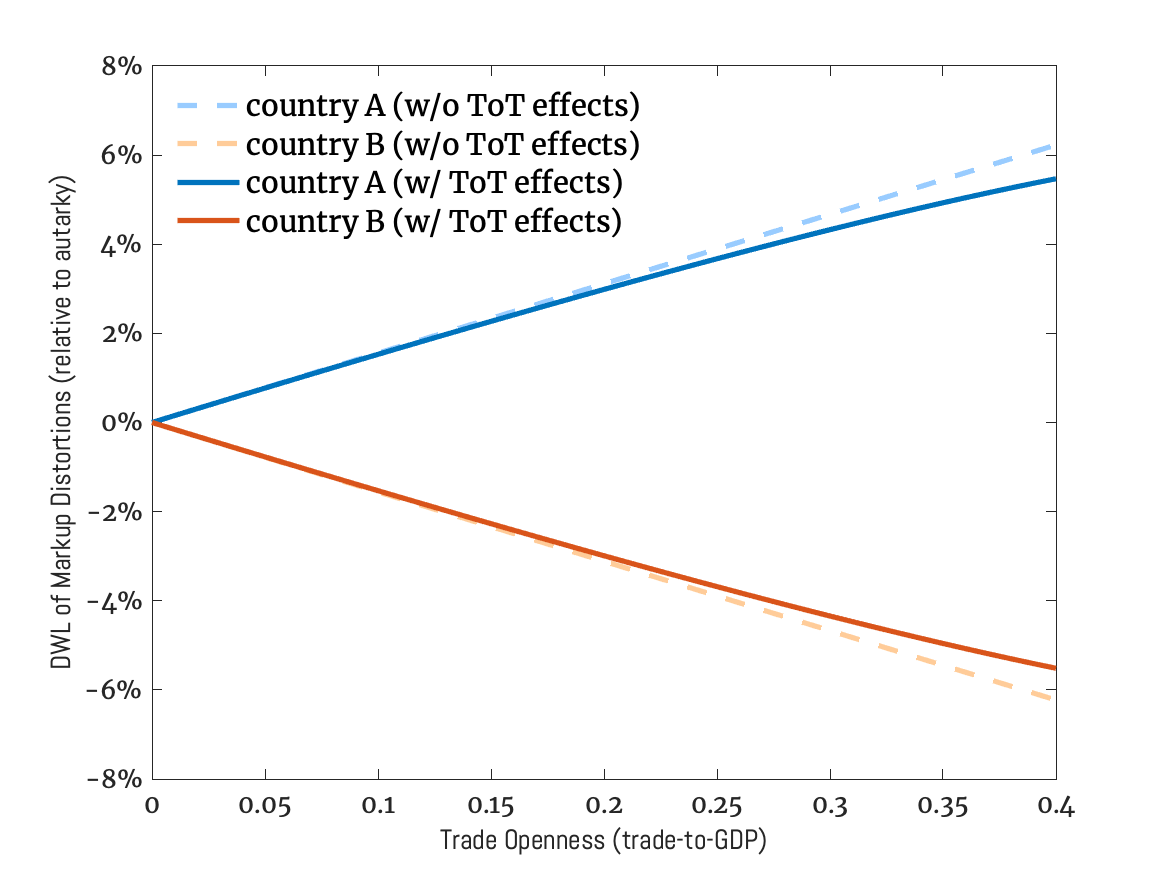
\includegraphics[scale=0.75]{numerical_simulation/numerical_wage_effects}
\par\end{centering}
\noindent\begin{minipage}[t]{1\columnwidth}%
\begin{singlespace}
\emph{Note}: This figure demonstrates that the factoral terms of trade
(ToT) effects associated with markup distortions are relatively small
compared to the direct welfare loss caused by these distortions. Specifically,
the figure illustrates that the welfare loss resulting from markup
distortions is nearly identical whether we consider the associated
wage effects (represented by the solid line) or measure the welfare
loss without accounting for wage effects (represented by the dashed
line). The figure is generated through numerical simulations of a
two-sector Krugman model with two countries, $A$ and $B$. Sector
2 has a higher markup ($\mu_{2}=1.5$) compared to Sector 1 ($\mu_{1}=1.1$).
Country $A$ has a revealed comparative advantage in the high-markup
sector, with $\lambda_{AB,2}=0.75$, $\lambda_{AB,1}=0.25$ , while
Country $B$ has a revealed comparative advantage in the low-markup
sector, with $\lambda_{BA,2}=0.25$, $\lambda_{BA,1}=0.75$. Both
countries have equal population sizes ($L_{A}=L_{B}$) and the same
Cobb-Douglas expenditure shares across sectors ($e_{A}=e_{B}=1/2$).
The trade elasticities in each sector are consistent with the underlying
markup, as per the Krugman model: $\theta_{1}=2$ and $\theta_{2}=10$.
In this numerical example, Country $A$'s pattern of revealed comparative
advantage aligns with that of high-income countries, while Country
$B$'s revealed comparative advantage is similar to that of low-income
countries, as manifested in real-world data.
\end{singlespace}
%
\end{minipage}
\end{figure}

\begin{figure}
\caption{\label{fig: free entry}The internationally zero-sum welfare consequences
of markup distortions under free entry}
\vspace{-5bp}

\begin{centering}
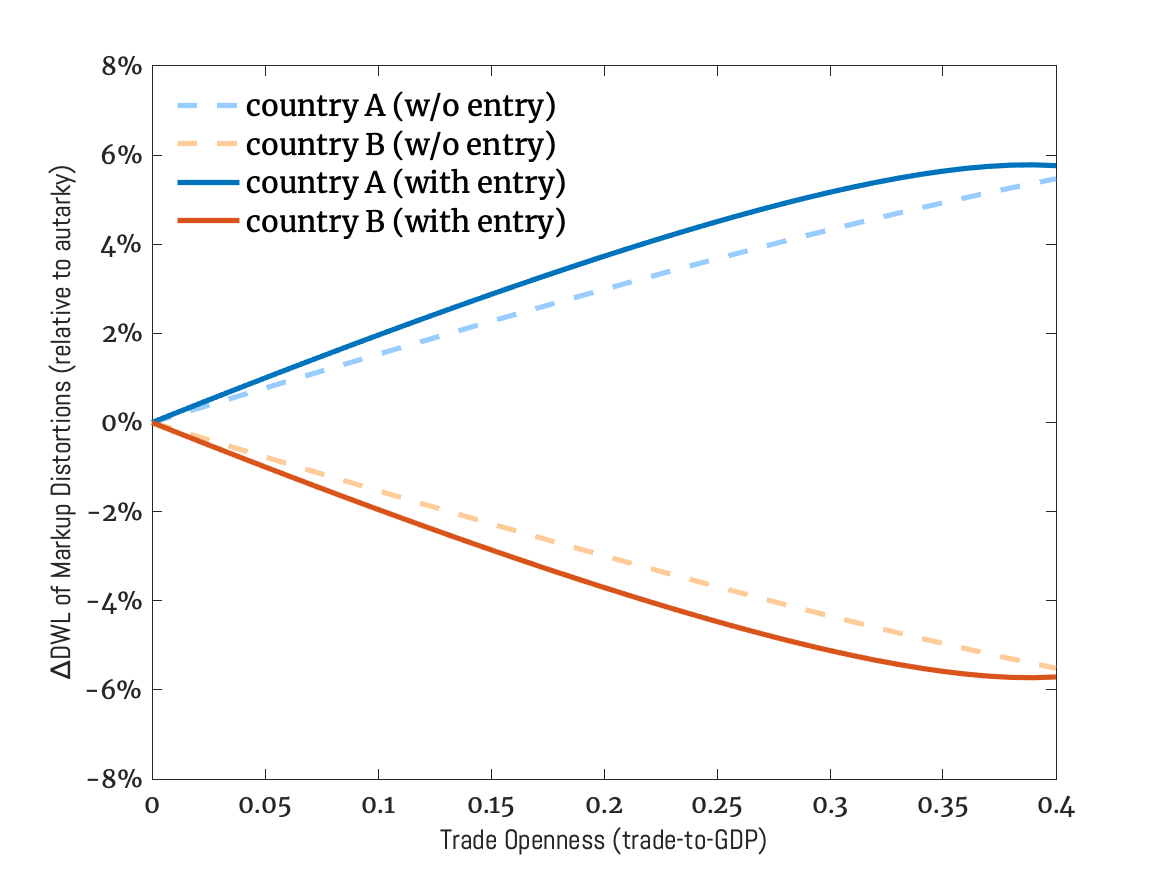
\includegraphics[scale=0.75]{numerical_simulation/numerical_free_entry}
\par\end{centering}
\noindent\begin{minipage}[t]{1\columnwidth}%
\begin{singlespace}
\emph{Note}: This figure demonstrates that the zero-sum welfare effects
of trade in markup-distorted economies persist even under free entry.
The lines represent the change in the welfare loss (DWL) of markups
as a function of increased trade openness, which is measured by a
higher trade-to-GDP ratio. This solid line corresponds to a scenario
with free entry. In contrast, the dashed line traces the change in
the welfare loss under restricted entry conditions, which is our baseline
specification. The figure is generated through numerical simulations
of a two-sector Krugman model with two countries, $A$ and $B$. Sector
2 has a higher markup ($\mu_{2}=1.5$) compared to Sector 1 ($\mu_{1}=1.1$).
Country $A$ has a revealed comparative advantage in the high-markup
sector, with $\lambda_{AB,2}=0.75$, $\lambda_{AB,1}=0.25$ , while
Country $B$ has a revealed comparative advantage in the low-markup
sector, with $\lambda_{BA,2}=0.25$, $\lambda_{BA,1}=0.75$. Both
countries have equal population sizes ($L_{A}=L_{B}$) and the same
Cobb-Douglas expenditure shares across sectors ($e_{A}=e_{B}=1/2$).
The trade elasticities in each sector are consistent with the underlying
markup, as per the Krugman model: $\theta_{1}=2$ and $\theta_{2}=10$.
In this numerical example, Country $A$'s pattern of revealed comparative
advantage aligns with that of high-income countries, while Country
$B$'s revealed comparative advantage is similar to that of low-income
countries, as manifested in real-world data.
\end{singlespace}
%
\end{minipage}
\end{figure}

\begin{figure}[!tbh]
\caption{\label{fig: markup} Distributions of firm-level markups across industries}
\vspace*{0in}
\begin{centering}
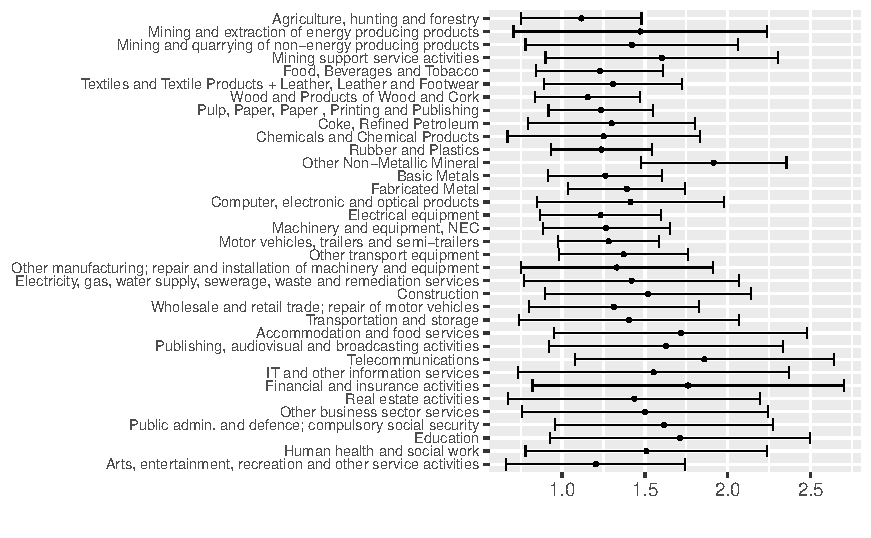
\includegraphics[scale=1.25]{WorldScope/figure/figure_markup}\vspace*{-0.25in}
\par\end{centering}
\noindent\begin{minipage}[t]{1\columnwidth}%
\begin{spacing}{0.8}
{\footnotesize\emph{Note}}{\footnotesize : The figure shows the within-industry
distribution of firm-level cost-based markups in 2010. The mean markup
of a given industry is graphed as a dot in the figure, while the error
bars that extend below and above the mean markup represent one standard
deviation below and above the mean, respectively.}
\end{spacing}
%
\end{minipage}
\end{figure}

\begin{figure}
\caption{\label{fig: markup-compariso}Within-industry markup comparison: \emph{high-income
vs low and middle income countries}}

\begin{centering}
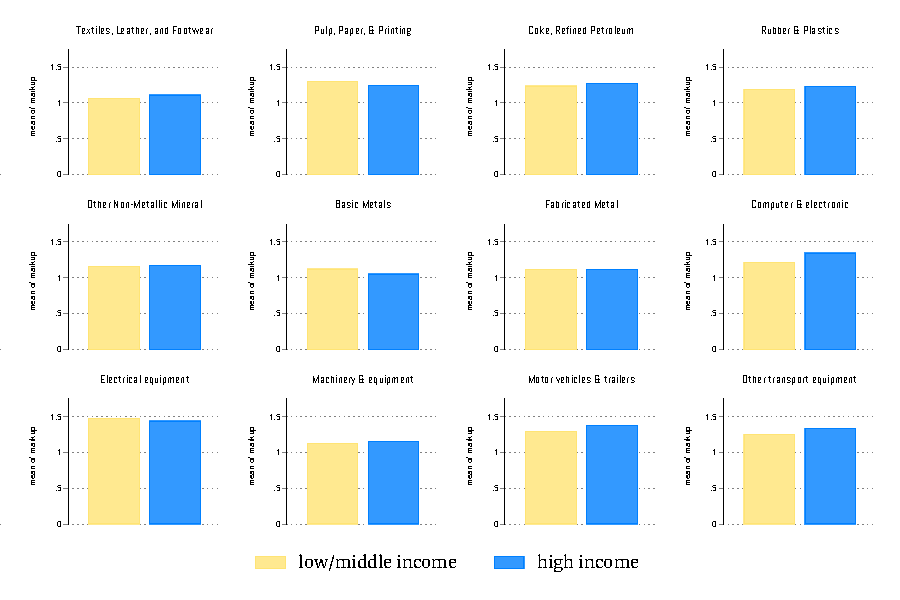
\includegraphics[scale=1.25]{WorldScope/markup_income/fig18}
\par\end{centering}
\noindent\begin{minipage}[t]{1\columnwidth}%
{\scriptsize\emph{Note}}{\scriptsize : This figure compares industry-specific
average markups between firms headquartered in high-income and low-/middle-income
economies. Consistent with our semi-parametric model\textquoteright s
prediction, the results indicate that markup distributions within
narrowly defined industries are nearly identical across income groups.
The markups are estimated using the cost-based approach and data from
}{\scriptsize\noun{WorldScope}}{\scriptsize{} covering years 2004 to
2016. High-income and low and middle income countries are defined
based on the classification of countries by the United Nations.}%
\end{minipage}
\end{figure}

\begin{figure}[!tbh]
\caption{\label{fig: F1 (IO linkages)} The welfare loss from market power
under IO linkages}

\vspace*{0.1in}
\begin{centering}
\includegraphics[scale=1.2]{\string"ICIO data/Decomposition/Fig_2_app\string".pdf}
\par\end{centering}
\noindent\begin{minipage}[t]{1\columnwidth}%
\begin{spacing}{0.8}
{\footnotesize\emph{Note}}{\footnotesize :}{\footnotesize\emph{ }}{\footnotesize The
above graph reports the welfare loss from market power averaged across
country groups. For example, a 5\% loss implies that markups lower
real consumption by 5\% relative to the efficient level. The figures
in the top panel are computed using Lemma 3 (which accounts for input-output
linkages) using annual data on markups and trade/expenditure shares.
The figures in the middle panel are computed by assuming that trade/expenditure
shares remain constant at their 2005 level. The figures in the bottom
panel are computed by assuming that markups remain constant at their
2005 level. Data on industry-level expenditure, trade, production,
and input-output shares are from the ICIO.}
\end{spacing}
%
\end{minipage}
\end{figure}

\begin{figure}
\caption{\label{fig: map appendix (a)}Trade-Induced change in welfare loss
from markups (exhibit A)}

\begin{centering}
\includegraphics[width=1\textwidth]{\string"ICIO data/Appendix_Figures_Tables/Figure_12/figure_worldmap_A\string".png}
\par\end{centering}
\begin{centering}
\includegraphics[width=1\textwidth]{\string"ICIO data/Appendix_Figures_Tables/Figure_12/figure_worldmap_B\string".png}
\par\end{centering}
\noindent\begin{minipage}[t]{1\columnwidth}%
\begin{singlespace}
{\small\emph{Note}}{\small : The map illustrates the unequal exposure
to profit-shifting externalities among high and low-income country
groups. It displays the per-cent change in the welfare loss of markups
due to international profit-shifting ($\triangle\mathscr{D}_{i}$)
on a country by country basis. The reported change in losses are calculated
using Proposition 2 and represent the average effect implied by the
demand-based and cost-based markup estimates. Data on national and
industry-level output and expenditure shares are from ICIO in 2015.}
\end{singlespace}
%
\end{minipage}
\end{figure}

\begin{figure}
\caption{\label{fig: map appendix (b)}Trade-Induced change in welfare loss
from markups (exhibit B)}

\begin{centering}
\includegraphics[width=1\textwidth]{\string"ICIO data/Appendix_Figures_Tables/Figure_12/figure_worldmap_C\string".png}
\par\end{centering}
\begin{centering}
\includegraphics[width=1\textwidth]{\string"ICIO data/Appendix_Figures_Tables/Figure_12/figure_worldmap_D\string".png}
\par\end{centering}
\noindent\begin{minipage}[t]{1\columnwidth}%
\begin{singlespace}
{\small\emph{Note}}{\small : The map illustrates the heterogeneous
exposure to profit-shifting externalities within high and low-income
country groups. It displays the per-cent change in the welfare loss
from markups due to international profit-shifting ($\triangle\mathscr{D}_{i}$)
on a country by country basis. The reported change in welfare losses
are calculated using Proposition 2 and represent the average effect
implied by the demand-based and cost-based markup estimates. The markups
levels are taken from our demand-based estimation. Data on national
and industry-level output and expenditure shares are from ICIO in
2015.}
\end{singlespace}
%
\end{minipage}
\end{figure}

\begin{figure}
\caption{\label{fig: Fig6}International patterns of profit-shifting}
\vspace*{-0.2in}
\begin{centering}
\includegraphics{\string"ICIO data/Fig4_Profit_Shifting/Fig4\string".pdf}
\par\end{centering}
\noindent\begin{minipage}[t]{1\columnwidth}%
\begin{singlespace}
{\small\emph{Note}}{\small : An arrow from country $i$ to $j$ corresponds
to the excess profits or rents collected by firms in country $j$
from consumers in country $i$ as a percentage of the profits collected
by domestic firms. Excess profits are calculated using sales data
from }{\small\noun{Icio}}{\small{} and markups estimated by applying
the cost-based methodology to }{\small\noun{Worldscope}}{\small{} data---both
in year 2010.}
\end{singlespace}
%
\end{minipage}
\end{figure}

\begin{figure}[!tbh]
\caption{\label{fig: Fig8}The welfare loss from market power under different
levels of cross-industry substitutability}

\begin{centering}
\includegraphics{\string"ICIO data/Appendix_Figures_Tables/Figure_10/Figure_10\string".pdf}
\par\end{centering}
\noindent\begin{minipage}[t]{1\columnwidth}%
\begin{spacing}{0.8}
{\footnotesize\emph{Note}}{\footnotesize : The above graph shows how
a higher substitution elasticity between industries amplifies the
aggregate loss from markups. Regarding units: a 5\% loss implies that
markups lower real consumption by 5\% relative to the efficient level.
Data on industry-level expenditure, trade, production, and input-output
shares are from the ICIO. Data on markups are based on our demand-based
markup estimates.}
\end{spacing}
%
\end{minipage}
\end{figure}


\end{document}
